%!TEX root = ../thesis.tex
%*******************************************************************************
%****************************** Second Chapter *********************************
%*******************************************************************************

\chapter{\ont{} sequencing for \mtb{} transmission clustering}
\label{chap:clustering}

\ifpdf
    \graphicspath{{Chapter2/Figs/Raster/}{Chapter2/Figs/PDF/}{Chapter2/Figs/}}
\else
    \graphicspath{{Chapter2/Figs/Vector/}{Chapter2/Figs/}}
\fi


%%%%%%%%%%%%%%%%%%%%%%%%%%%%%%%%%%%%%%%%%%%%%%%%%%%%%%%%%%%%%%%%%%%%%%%%%%%%%%%%%
%%%%%%%%%%%%%%%%%%%%%%%%%%%%%%%%%%%%%%%%%%%%%%%%%%%%%%%%%%%%%%%%%%%%%%%%%%%%%%%%%
\setcounter{section}{-1}
\section{Publication and collaboration acknowledgements}
\label{sec:ch2-acknowledge}

A manuscript comprising the work in this chapter and \autoref{chap:dst} is currently in preparation. The only work that was not completed by myself is the DNA sequencing of the samples.
The DNA extractions and Illumina and \ont{} sequencing for the samples from Madagascar was conducted by Marie Sylvianne Rabodoarivelo and Simon Grandjean Lapierre. The Next Generation Genomics Core within Cold Spring Harbor Laboratory performed the PacBio sequencing for these samples.

\towrite[inline]{acknowledge the people who did the south african sequencing}

\towrite[inline]{acknowledge the people who did the birmingham sample sequencing}

Fan Yang-Turner of the Nuffield Department of Medicine, University of Oxford, performed the variant-calling of all Illumina samples. 

While I did the bioinformatic work (except the Illumina variant-calling) in this chapter, I must acknowledge the excellent guidance I have received. My supervisor Zamin Iqbal who always knows the right questions to ask. Simon Grandjean Lapierre helped conceive of this study, along with Zam, and whose clinical perspective helped keep me grounded in the real world. I would also like to acknowledge the many insightful conversations with our other collaborators: Marie Sylvianne Rabodoarivelo, Anastasia Koch, Niaina Rakotosamimanana, Anzaan Dippenaar, and Helen Cox. Furthermore, Tim Peto, whose input helped shape some of the clustering evaluation.

%=========================================================================

\section{Introduction}
\mtb{} is a contagious bacterial pathogen that causes the disease Tuberculosis (TB). It accounts for more deaths than any other pathogen each year \cite{who2020} — as such, detecting chains of \mtb{} transmission is of the utmost importance. Whole-genome sequencing (WGS) has established itself as a vital tool for identifying possible transmission clusters and is being used by some leading public health agencies to aid contact tracing \cite{phe-tb-england,brooks2020}. Illumina is considered the gold standard for this type of WGS work. However, Illumina is not readily available in many high-burden TB settings and requires considerable time and resources to start and maintain. \ont{} has shown itself to be adept in these types of settings, having been used to notable effect during recent Zika \cite{faria2016} and Ebola \cite{quick2016,Hoenen2016} outbreaks. Even in environments where resource availability is not an obstacle, \ont{}'s rapid turnaround time has been used for monitoring COVID-19 and informing infection control measures \cite{meredith2020}. The time and resources required to set up \ont{} sequencing are far lower than Illumina, but despite this, there has been little work done to assess its suitability for \mtb{} WGS-based transmission clustering. The lack of work in this space likely stems from the long-held belief that due to its higher sequencing error rate, \ont{} is not capable of such fine-grained analyses. However, \ont{} has seen considerable improvements in its accuracy in recent years \cite{wick2019}, and studies using variant calls from the technology are becoming increasingly common \cite{sanderson2020,watson2020}. In particular, Public Health England (PHE) has investigated the use of \ont{} for the analysis of Shiga toxin-producing \ecoli{} and found it to be well-suited to the application \cite{greig2021}. 

In this chapter, we evaluate whether \ont{} sequencing can provide \mtb{} transmission clusters consistent with Illumina. To facilitate this investigation, we collect a new dataset of 150 samples - from Madagascar, South Africa, and England - sequenced on both Illumina and \ont{} platforms. We first assess \ont{} variant calls and outline a filtering strategy to provide Illumina-level precision. Next, we use these variant calls to cluster samples based on SNP (single nucleotide polymorphism) distance thresholds and find \ont{} does not miss any samples from their expected cluster. Finally, we confirm that reliable clustering of samples from a mixture of Illumina and \ont{} modalities is achievable.

\mtb{} has a "closed" pan-genome; all species members share most (but not all) gene content. In \autoref{chap:denovo} we sought to improve variant calling of bacterial pan-genomes with genome graphs. The work in that chapter concentrated on \ecoli{}, which has an "open" pan-genome. In the interest of understanding how such genome graph methods can aid in closed pan-genomes, we additionally assess transmission clusters produced from \pandora{} variant calls. We construct two \mtb{} reference graphs from different densities of population variation towards this end. While the clustering from \pandora{} does not perform to the standards of the single-reference caller BCFtools, we gain many insights for the improvement of \pandora{} and the construction of genome graphs.

%=========================================================================

\section{Dataset}
\label{sec:ch2-dataset}

The data used for the work in this chapter, and \autoref{chap:dst}, are patient-derived \mtb{} isolates from culture. We gathered samples from Madagascar (118), South Africa (83), and England's National Mycobacteria Reference Service in Birmingham (46), giving us a total of 247 samples.  
Each sample was sequenced on both \ont{} and Illumina platforms. We aimed to perform all sequencing for a sample from a single DNA extraction. Performing all sequencing on the same DNA extract ensures that any variation identified between technologies for the same sample would be due to differences in the sequencing platform and not \textit{in vitro} evolution.  
As these samples are not reference isolates, and we want to be able to compare both Illumina and \ont{} to a "truth", we also sequenced 35 of the Malagasy isolates with PacBio.

\subsection{Illumina sequencing}

\subsubsection{Madagascar}

\todo[inline]{have emailed collabs}

\subsubsection{Birmingham}

\todo[inline]{assigned to zam}

\subsubsection{South Africa}

\improvement[inline]{tidy up as this is just copy-pasted from email from Anzaan}

Isolate selection \\
Clinical Mycobacterium tuberculosis (Mtb) isolates routinely collected in the Western Cape Province of South Africa, processed by the National Health Laboratory Service (NHLS) and diagnosed as rifampicin resistant tuberculosis, are biobanked at the South African Medical Research Council Centre for Tuberculosis Research (SAMRC-CTR) housed at the Division of Molecular Biology and Human Genetics at Stellenbosch University, South Africa. A convenience data set of 82 clinical Mtb isolates for which Illumina whole genome sequencing data was available were selected for Nanopore Sequencing.  

DNA extraction \\
% citation for this subsubsection
% Warren, R. et al. Safe Mycobacterium tuberculosis DNA extraction method that does not compromise integrity. J Clin Microbiol 44, 254-256, doi:10.1128/JCM.44.1.254-256.2006 (2006).
Clinical Mtb isolates were cultured on supplemented 7H10 solid media under BSL3 conditions. Phenol-chloroform DNA extraction was performed on heat inactivated cultured isolates as previously described(CITE). 

WGS (Illumina) \\
% note from anzaan
% Many of these WGS will be published soon. I am waiting for the final list and then I’ll include their accession numbers so that we can refer to them here. If all were published, we also don’t have to upload them to ENA (or which ever data repository)
Paired-end genomic libraries were prepared using the Illumina Nextera XT library or NEBNext Ultra TM II FS DNA Library Preparation Kits (Illumina Inc, San Diego, CA, USA) according to the manufacturers’ instructions. Pooled samples were sequenced on an Illumina HiSeq2500 or NextSeq500 instrument.

\subsection{\ont{} sequencing}

\subsubsection{Madagascar}

\todo[inline]{have emailed collabs}

\subsubsection{Birmingham}

\todo[inline]{assigned to zam}

\subsubsection{South Africa}

\improvement[inline]{tidy up as this is just copy-pasted from email from Anzaan}

Remnant stored DNA used for Illumina WGS from each isolate was retrieved from storage and used for Nanopore library preparation. Per isolate, one microgram of undigested DNA was prepared for Nanopore Sequencing using the ligation sequencing kit (SQK-LSK109). The native barcoding expansion kit (EXP-NBD104) was used for multiplexing. The protocols for sequencing genomic DNA by ligation and native barcoding were carried out according to the manufacturers’ instructions. Multiplexed sequencing libraries consisted of 6-12 barcoded DNA samples, and all libraries were sequenced using SpotON R9.4.1 flow cells on a MinION device. 

\subsubsection{Preprocessing}

All \ont{} data for this project was basecalled and de-multiplexed using the \ont{} proprietary software tool \guppy{} (version 3.4.5). We used default parameters for basecalling, and the only non-default parameter used for de-multiplexing was to trim barcodes from the resulting sequences.  

\subsection{PacBio sequencing}
Thirty-five of the Malagasy samples were sequenced and processed at the Next Generation Genomics Core within Cold Spring Harbor Laboratory with PacBio Sequel 1M V2 SMRT cells. The circular consensus was generated via the SMRTlink graphical user interface version 6.0.0.47841. \autoref{app:pacbio-seq} outlines the full details of the sequencing protocol.

%=========================================================================

\section{High-quality genome assemblies for validating variant calls}
\label{sec:asm_results}
A central component of the work in this chapter is validating the quality of variant calls - without being biased by assuming short reads are the "truth". In \autoref{sec:var-calls} we compare the precision and recall of \ont{} and Illumina variant calls. A necessary component of such analysis is a reference genome for each sample. Thirty-five of the Malagasy samples in the dataset were sent for PacBio Circular Consensus Sequencing (CCS) in addition to the matched sequencing on both the \ont{} and Illumina platforms. PacBio CCS produces so-called high-fidelity sequencing reads with a base-level accuracy greater than 99.8\% \cite{wenger2019}. These reads have such a high accuracy because each one is the consensus from multiple passes of the DNA enzyme around a circular copy of the original double-stranded read. As the CCS reads are both long and accurate, they are regularly used to produce high-quality \denovo{} assemblies and complete existing reference genomes \cite{garg2021,masonbrink2021}. For the samples with available PacBio data, we construct high-quality assemblies to use as reference genomes.

We chose samples with greater than 30x coverage across all three sequencing technologies to produce high-quality assemblies. In total, this left us with 9 Malagasy samples. There have been many new genome assembly methods produced since the last known assessment of \mtb{} long-read assemblies \cite{bainomugisa2018}. As such, we benchmark five assemblers and select the best for each sample. The reason for this comparison is that different assembly algorithms can produce quite varied results depending on sequencing technology used, species, or computational resource availability \cite{wick2020,demaio2019}. The assembly tools used were Canu (v2.0;\cite{koren2017,nurk2020}), Flye (v2.8;\cite{flye2019}), Unicycler (v0.4.8;\cite{wick2017}), HASLR (v0.8a1;\cite{haslr2020}), and Spades(v3.14.0;\cite{antipov2016}). \autoref{app:asm} presents the complete benchmark.

In summary, we use the unpolished PacBio-only assemblies produced by \flye{} as reference genomes for eight samples. Although we assembled nine samples, we exclude one from further analysis due to significant contamination.

%=========================================================================

\section{Quality control}
\label{sec:ch2-qc}

Before any variant calling, all samples were subjected to a quality control (QC) pipeline to ensure all data used was of the highest quality. 

The first step in this QC was decontamination of both Illumina and \ont{} sequencing reads. We use the decontamination database from \vrb{clockwork} (\url{https://github.com/iqbal-lab-org/clockwork}), which contains a wide range of organisms, including viral, human, \mtb{}, Nontuberculous Mycobacteria (NTM), and nasopharyngeal-associated bacterial genomes. Each genome has associated metadata indicating if it is contamination or not. Next, reads are mapped to the database using \vrb{bwa mem} (Illumina;v0.7.17) \cite{li2013} and \vrb{minimap2} (\ont{};v2.17) \cite{li2018}. We quantify the proportion of reads considered contamination, unmapped, and wanted with the resulting alignment. A read is wanted if it has any mapping to a non-contamination genome (\mtb{}) in the database and is output to a final decontaminated fastq file. All other reads are considered contamination. 

All decontaminated fastq files were randomly subsampled to a depth of 60x (Illumina) and 150x (\ont{}) using \vrb{rasusa} \cite{rasusa2019}. The reason for subsampling is to limit large read sets that can drastically slow down later steps in the analysis process and do not provide any benefit \cite{demaio2019}. Any sample with a depth less than the maximum threshold remains unchanged by this subsampling.  

The last step in the QC pipeline is to assign lineages for each sample. A panel of lineage-defining SNPs \cite{Shitikov2017,Rutaihwa2019,stucki2016} is used in conjunction with a sample's Illumina VCF from \autoref{sec:illumina-var-call} for the lineage assignment. At each lineage-defining position in the sample's VCF, we determine if the called allele is the same as the panel allele. If it is, we add the full lineage that allele defines (e.g. $4.1.1$) to a list of called lineages. We abandon lineage assignment for a sample if more than one heterozygous call is made at lineage-defining positions. After classifying all of a sample's lineage-defining positions, we then produce a lineage assignment based on the list of called lineages. We use the most recent common ancestor of all the called lineages as the lineage assignment. For example, if the called lineages are $[4, 4.2.3, 4.2.5]$, the lineage assignment would be $4.2$. Finally, a mixed-lineage assignment is made if more than one called lineage is from a different major lineage group. For example, $[4, 4.2.3, 4.2.5, 3.2]$ would still be called lineage $4.2$; however, $[4, 4.2.3, 4.2.5, 3.2, 3.1]$ would be deemed mixed.

The purpose of QC is to ensure that all samples used in later analyses are of the highest quality. By highest quality, we mean all samples have perfectly matched Illumina and \ont{} data, sufficient read depth of coverage on both sequencing technologies (Illumina $\ge 20$ and \ont{} $\ge 30$), no contamination, and no evidence of a mixed \mtb{} population. Fifty-eight samples failed to pass our QC measures, and 39 had non-matched Illumina and \ont{} data. One of the samples that failed QC is part of the eight PacBio samples we generated assemblies for in \autoref{sec:asm_results} - we exclude this sample from any further analysis. In total, we use the 150 samples that have passed QC in the remainder of this chapter and \autoref{chap:dst}.

%=========================================================================

\section{Construction of \mtb{} reference graphs}
\label{sec:tbprg}
A parallel line of investigation in this chapter is to assess the applicability of \pandora{} (see \autoref{chap:denovo}) to species with a closed pan-genome, such as \mtb{}. \pandora{} requires a population reference graph (\prg{}) in order to operate. For the work in this chapter, we chose to construct a reference \prg{} based on the \mtb{} reference genome, H37Rv (accession NC\_000962.3). We add variants sampled from 15,211 global \mtb{} isolates gathered by the \cryptic{} consortium(\todo{CITE}). We sampled at two different rates to evaluate how varying complexity of \prg{}s affect variant-calling precision and recall.

To ensure the reference \prg{} is not biased towards a particular lineage, we first split the global \cryptic{} VCF into separate lineage VCFs. We assign lineages for each of the global samples using the same approach as in \autoref{sec:ch2-qc}. Lineages 1-4 were split into separate VCF files, and all other lineages were grouped into a single VCF due to a much smaller representation. Variant calls from 14 high-quality \mtb{} assemblies, representing lineages 1-7, were also included in this "other" lineage VCF(CITE). The two \prg{} complexities we construct were termed "sparse" and "dense". From each lineage VCF, we took a random subsample of 50 and 200 samples and combined them into single sparse and dense VCFs, respectively. Note, we use the same fixed random seed for the subsampling to ensure the sparse \prg{} is a subset of the dense \prg{}. Finally, we filtered the resulting VCFs to remove any positions with no alternate allele calls or that failed the filtering applied by the \cryptic{} pipeline \vrb{clockwork} (except for masked positions).  

The reference \prg{} that \pandora{} uses is actually a collection of local \prg{}s (loci). These loci are effectively partitions of the original genome; one can partition based on any criteria they like. We chose to split the H37Rv genome based on the genomic features outlined in the accompanying General Feature Format (GFF) file from the NCBI database. We also retain the segments \emph{between} the features - so-called intergenic regions (IGRs). We combine genomic features with overlapping coordinates (e.g., transcribed on opposite strands or different reading frames) into a single locus and join any locus (feature or IGR) shorter than 500bp with its 3' neighbour. By building the reference \prg{} in this manner, we ensure representation of every position in the H37Rv genome amongst all loci. We then remove any locus with 30\% or more of its positions overlapping a genome mask of repetitive regions in H37Rv \cite{tbmask2014}. Refer to \autoref{app:mask} for a detailed description of how we chose this masking strategy.

We form the sparse and dense \prg{}s by applying the variants from the respective VCF to the template (reference) sequence of each locus; for each position in the VCF, we infer the locus it corresponds to. We then take all (called) alternate alleles and create a sequence for each; that is, the template sequence, with the reference allele replaced by the alternate allele. Note, we disregard any indels longer than 20bp or that span a locus boundary. Finally, all of these sequences are pooled into a single fasta file for each locus. 

The multi-sequence fasta file for each locus is then subjected to multiple sequence alignment (MSA) using MAFFT (v7.471; \cite{nakamura2018}). We use the accurate global alignment setting, G-INS-i \cite{katoh2016}, with default parameters, using the \vrb{ginsi} script provided with MAFFT. The resulting MSA is then converted to a \pandora{}-compatible \prg{} using the \makeprg{} program (v0.1.1; \todo{CITE}) with a maximum nesting level of 5 and minimum match length of 7. All of the local \prg{}s are then combined into a single \prg{} file and indexed with \pandora{} using a \kmer{} size of 15 and window size of 14. In the end, we have two \prg{} files - sparse and dense.

\subsection{Computational performance}
\label{sec:tbprg-comp-perf}

An important consideration for the usability of any genomic method is the computational cost in terms of time and memory resources. The construction process just outlined need only be run once, and then it can be used as a reference for subsequent \pandora{} usage. However, it is necessary to understand the time and resources required in order to identify bottlenecks. Additionally, if the resource usage is high enough, it may also limit who can build a reference graph. We outline the time and memory requirements for each step of the graph construction in \autoref{tab:build-prg}. All times are on a single compute node with 32 CPU cores. We only report the MSA, \makeprg{}, and \pandora{} index steps as these are necessary steps; those preceding use little time and memory and can be done in several different ways.

\begin{table}
\centering
\begin{tabularx}{\textwidth}{|l|X|X|X|X|X|X|}
\hline
         & \multicolumn{3}{l|}{Sparse}                          & \multicolumn{3}{l|}{Dense}                           \\ \hline
Step     & CPU time (sec) & Real time (H:m) & Max. RAM (GB) & CPU time (sec) & Real time (H:m) & Max. RAM (GB) \\ \hline%\cline{1-2} \cline{4-5} \cline{7-7} 
MSA      & 138576         & 1:16             & 209              & 445284         & 3:56             & 301              \\ \hline%\cline{1-2} \cline{4-5} \cline{7-7} 
Make PRG & 3746           & 0:04             & 0.9              & 4269           & 0:05             & 0.9              \\ \hline%\cline{1-2} \cline{4-5} \cline{7-7} 
Index    & 142            & 0:01             & 1.5              & 361            & 0:01             & 1.7              \\ \hline%\cline{1-2} \cline{4-5} \cline{7-7} 
\end{tabularx}
\caption{Computational time and memory (RAM) usage for the main steps of building a \mtb{} reference graph. Sparse and Dense refer to two different densities with respect to the number of variants used. All steps were run on a single compute node with 32 CPU cores. MSA=multiple sequence alignment;PRG=population reference graph.}
\label{tab:build-prg}
\end{table}

%=========================================================================

\section{Variant calling and filtering assessment}
\label{sec:var-calls}
One approach to determining genetic distance is to count the number of SNPs that differentiate two samples. These distances enable the inference of likely transmission clusters based on some predefined number of expected SNPs. Filtering of variant calls is integral to creating trusted variant calls on which to base such distances. However, there are many such filters used for Illumina genomic data, and they can produce inconsistent results \cite{walter2020}. As our focus is on whether \ont{} can be used for public health applications, we utilise the PHE Illumina pipeline - COMPASS \cite{Jajou2019} - as a comparison.

Before attempting to define SNP thresholds for \ont{} data, we explore the impact of a range of filtering parameters for both \bcftools{} and \pandora{}. The aim of this filter calibration is ultimately to determine if SNP-calling precision for \ont{} is comparable with Illumina, and if not, how close can we get it.

We evaluate the resulting, filtered SNP calls against the COMPASS Illumina SNP calls for the seven samples with high-quality PacBio assemblies (see \autoref{sec:asm_results}) to ensure no bias for Illumina or \ont{}. For others interested in investigating variant filters for \ont{} data, we also hope this calibration acts as a good starting point for deeper analysis.

\subsection{Validating variant calls}

We evaluate the precision and recall of SNP calls using the method outlined in \todo{link to varifier stuff in chapter 1} - \vrb{varifier} - with a flank length of 100bp. The samples we evaluated are those seven with PacBio assemblies that passed QC. As a truth genome for each, we use the unpolished \flye{} PacBio assembly, along with a mask for low-quality regions. These low-quality regions were identified by aligning the sample's Illumina reads to the assembly with \vrb{bwa mem} and flagging any position with less than 10 reads mapping to it or less than 90\% agreement (see \autoref{app:asm_disagree}). 

\subsection{Illumina variant calling}
\label{sec:illumina-var-call}

Fan Yang-Turner performed the Illumina variant calls (see \autoref{sec:ch2-acknowledge}) with the COMPASS pipeline used by PHE. Briefly, reads are mapped to H37Rv, and \vrb{samtools mpileup} is used to identify SNPs \cite{samtools2009}. SNPs are filtered based on the following criteria: i) must have at least five high-quality supporting reads, ii) must have at least one read in each direction, iii) 75\% of reads must be high-quality, iv) the diploid genotype must be homozygous, v) fraction of reads supporting the major allele must be at least 90\%. In addition, any SNPs falling within masked sites - as defined by aligning the H37Rv to itself and identifying repetitive regions \cite{tbmask2014} - are excluded. This mask is the same as in \autoref{sec:tbprg}.

\subsection{\ont{} variant calling: BCFtools}
\label{sec:bcftools-filters}

As there is no standard variant caller used for \mtb{} \ont{} data, we chose to use BCFtools (v1.11; \cite{bcftools2021}), as it has a long history of use in bioinformatics and is one of the main variant callers used for Illumina data. It is readily available to all users and is much more user-friendly than other available tools, some of which have only be trained on Human data \cite{clair2020}, or require the raw \ont{} data \cite{nanopolish2015}. Another main reason for its use is that it is the updated form of the \vrb{samtools} pipeline used by COMPASS and thus provides a somewhat "fair" comparison.

\ont{} reads were aligned to the H37Rv using \vrb{minimap2}, with options to produce SAM output containing no secondary alignments. The resulting SAM file is provided as input to the \bcftools{} subcommand \vrb{mpileup} with the option to skip indels. The resulting pileup is then used to call SNPs with \vrb{bcftools call} using the multiallelic caller with a haploid model and an option to skip indels.

There are many fields in the resulting VCF relating to the information about the reads that support each position. After a thorough examination of how filtering based on each field impacts precision and recall, we settled on five filters for \bcftools{}. First, we filter out positions with a quality (QUAL field) score less than 60. The quality is a log-scaled probability for the assertion made by the alternate allele. Second, a read position bias (RPB) of at least 0.05 is required. RPB indicates a bias for support from the ends of reads, as they are usually low quality. Third, we filter out positions with a segregation-based metric (SGB) less than -0.5. SGB is a measure of how read depths across alleles match expected depths. Fourth, variant distance bias (VDB) less than 0.002 is filtered out. VDB measures whether a variant's position is randomly distributed within the reads that support it or biased (e.g. near the start). Fifth, the fraction of reads supporting the called allele (FRS) must be 90\% or more.

\autoref{fig:bcftools-filters} shows how the addition of each of these filters impacts precision (proportion of calls that are correct) and recall (proportion of variants found) for \bcftools{} compared with COMPASS (Illumina). The trade-off between precision and recall is dependent on the question one is trying to answer. For transmission clustering, we place greater importance on precision as we seek to ensure the SNPs used are of the highest quality. The consequence of this is we miss some variants - compared to COMPASS.

The filtering we use for the remainder of the transmission inference
work is to apply all five filters mentioned above. These filters, represented by the yellow box in \autoref{fig:bcftools-filters}, lead to median precision and recall of 99.94\% and 84.26\%, respectively for the seven validation samples with PacBio assemblies. This is compared to the COMPASS median precision and recall values of 100\% and 92.58\%, respectively.

In summary, we produce \ont{} variant calls with equivalent precision to Illumina but with less recall.

\begin{figure}
\begin{center}
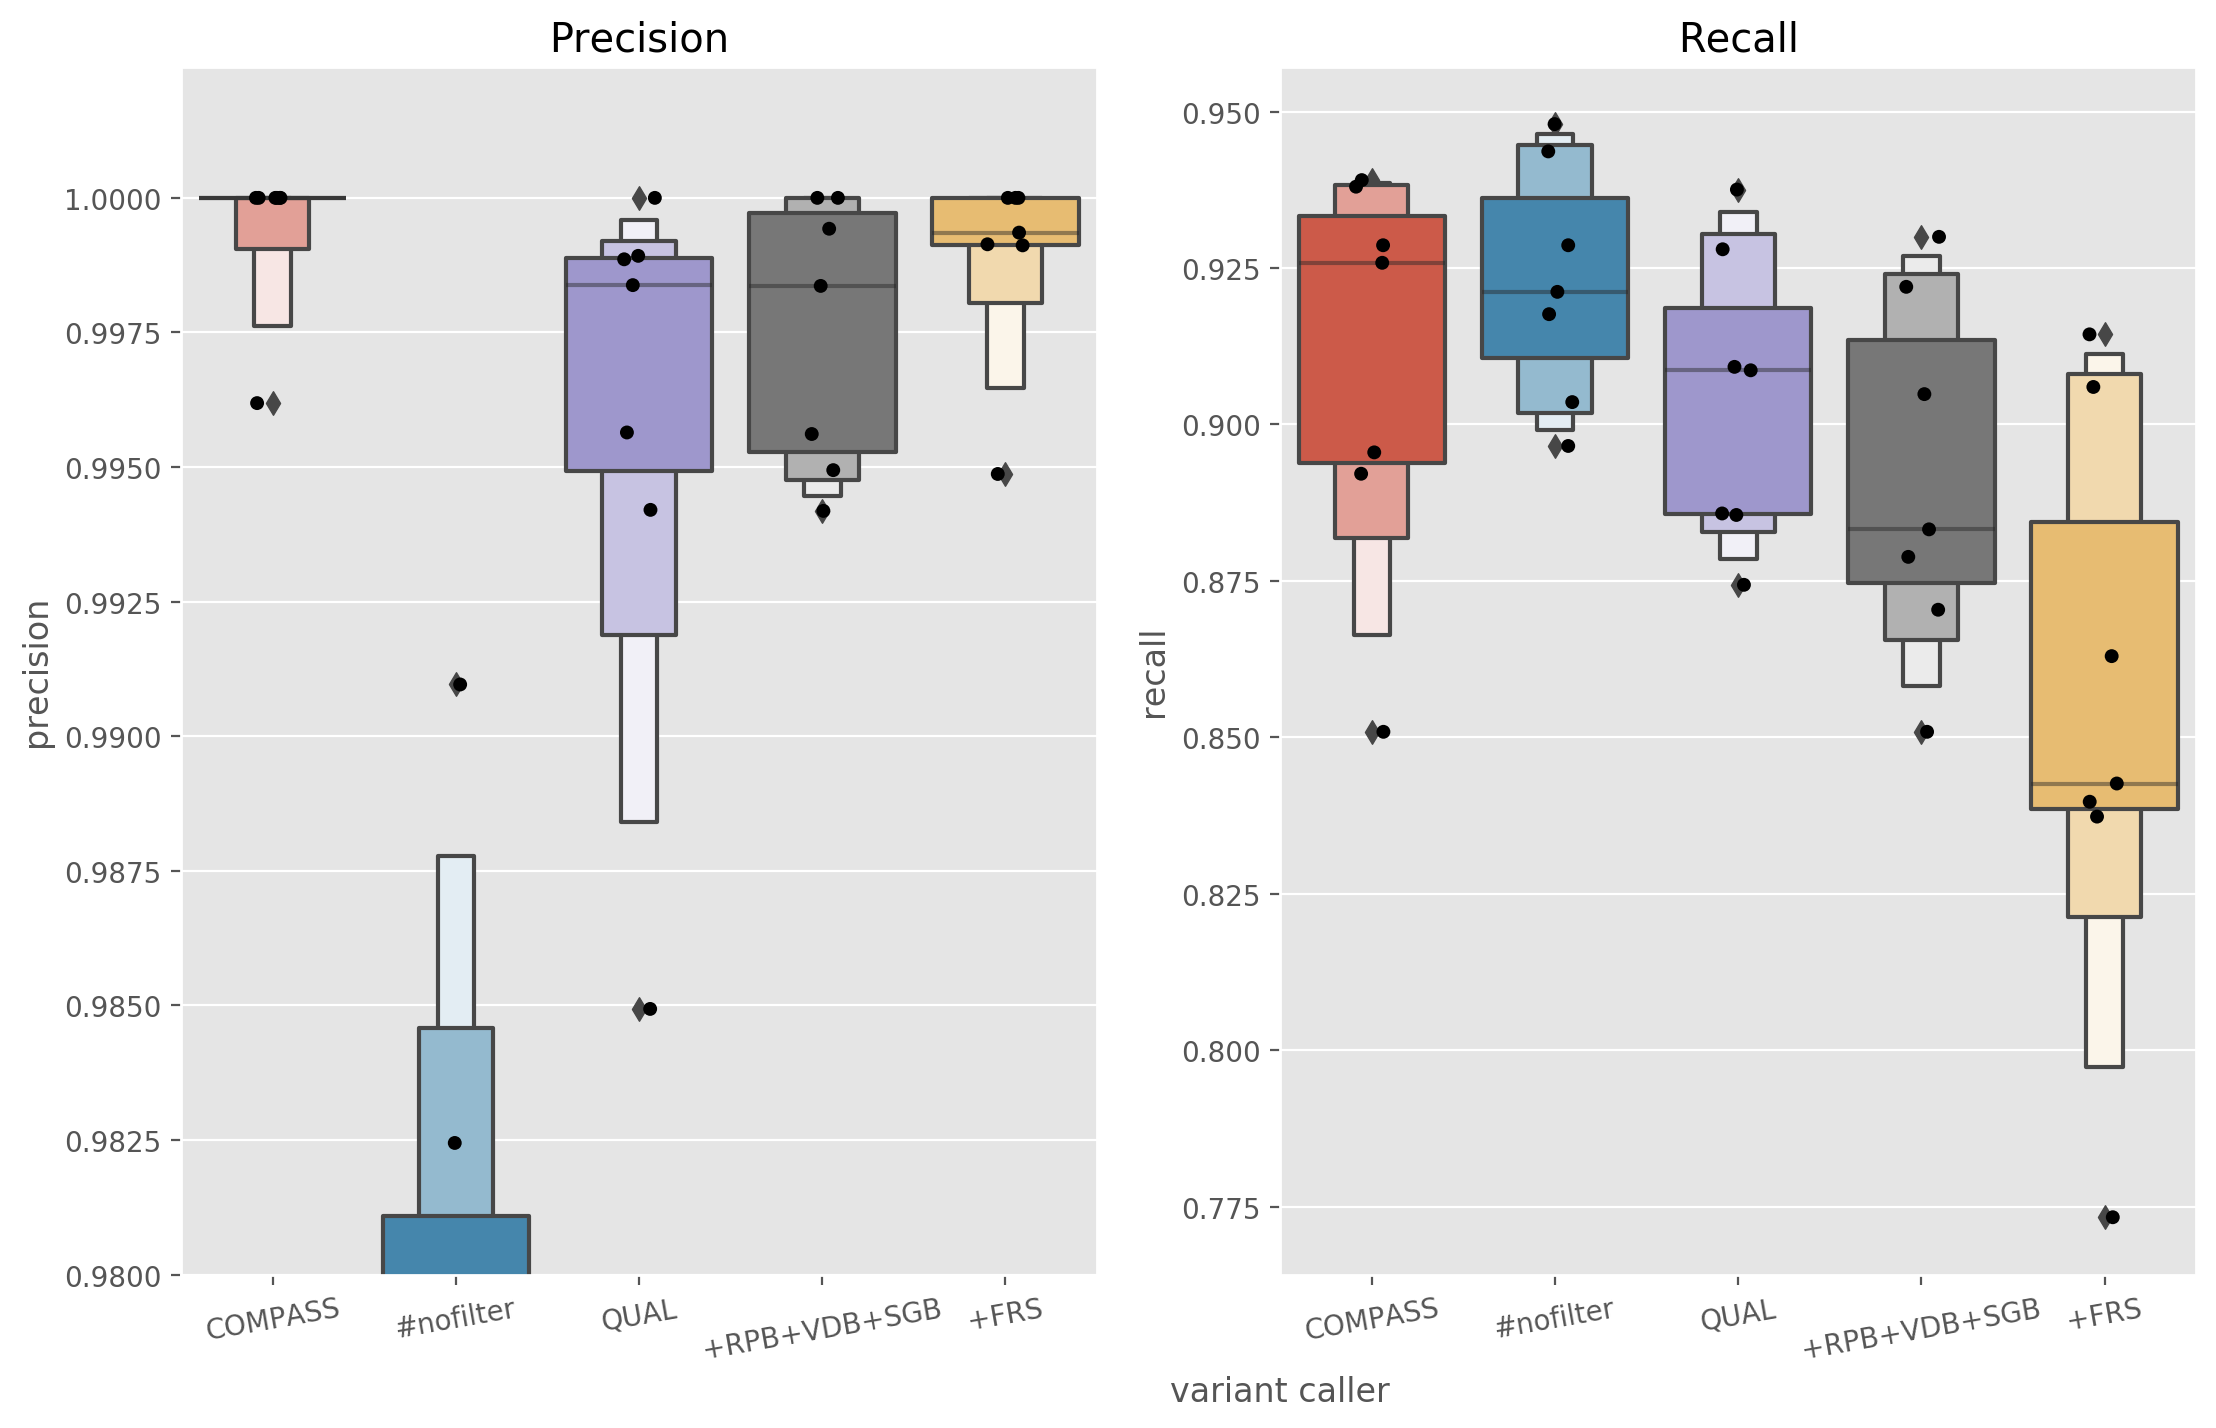
\includegraphics[width=0.90\columnwidth]{Chapter2/Figs/bcftools-precision-recall-filters.png}
\caption{{Precision (left) and recall (right) of SNPs for COMPASS (red) and a selection of \bcftools{} filters. \vrb{\#nofilter} (blue) is \bcftools{} with no filtering of variants. \vrb{QUAL} (purple) is \bcftools{} SNPs with a quality score of 60 or more. \vrb{+RPB+VDB+SGB} (grey) indicates \bcftools{} variants with the INFO field values $\ge 0.05$, $\ge 0.002$, and $\le -0.5$, respectively, plus QUAL. \vrb{+FRS} (yellow) shows \bcftools{} SNPs with all previous filters, plus only SNPs where the fraction of reads supporting the variant is at least 90\%. Note: the precision plot y-axis was cut causing some \vrb{\#nofilter} points to be hidden.
{\label{fig:bcftools-filters}}
}}
\end{center}
\end{figure}

\subsection{\ont{} variant calling: Pandora}
\label{sec:pandora-filters}

When assessing the best filters for increasing the precision of variant calls from \pandora{}, we are also interested in determining whether \prg{} density has a noticeable impact on performance. Therefore, we use the sparse and dense \prg{}s from \autoref{sec:tbprg} and look at the precision and recall these produce for the same filters.

\subsubsection{Single-sample}
\label{sec:map-var-calls}

For each sample, we discover \denovo{} variants using the method outlined in \autoref{chap:denovo} using the \vrb{discover} command of \pandora{} (version 0.8.0). We use default parameters, except limiting the number of novel variants from a candidate region to 10. Novel variants are added to the original MSAs from \autoref{sec:tbprg} with the \vrb{--add} routine in MAFFT \cite{katoh2012}. Next, \makeprg{} is run on the subsequent alignments, and the resulting updated \prg{} is indexed with \pandora{}. Finally, the \vrb{map} routine of \pandora{} genotypes a sample's reads and produces a VCF. To be able to compare the \pandora{} VCF to the truth assemblies, we instruct \pandora{} to output coordinates with respect to the H37Rv reference sequence for each locus. Running \pandora{} in this way leads to some alleles being quite long and redundant, so we use \vrb{bcftools norm} to trim unused alleles and reduce variants down to their most succinct representation. 

We apply four filters to the \pandora{} variant calls. First, there must be at least 3 reads supporting the called allele. Second, we keep positions with a strand bias of at least 1\%, which is the lowest depth on the forward or reverse strand divided by the total depth. Third, a genotype confidence score no less than 5. Fourth, the fraction of reads supporting the called allele (FRS) must be at least 90\%  - calculated the same way as in \autoref{sec:bcftools-filters}.

The results of incrementally applying these filters, along with no filters and COMPASS, are shown in \autoref{fig:pandora-filters-snps}. Of the two \prg{}s used, \pandora{}'s best median precision (100\%) is with the sparse \prg{} and all filters applied. With all filters, the sparse \prg{} leads to a median recall of 71.99\%. When compared to the COMPASS median precision and recall values of 100\% and 92.58\%, respectively, \pandora{} produces \ont{} SNP calls with equivalent precision to Illumina, but with 20.59\% less recall (SNPs \emph{and} indels are assessed in \autoref{app:pandora-all-vars}). Part of the recall disparity between \pandora{} and COMPASS is explained by the masking of loci in the reference graph (see \autoref{sec:tbprg} and \autoref{app:mask}). Despite this large difference in recall, we chose to use all of the filters outlined above because, as mentioned earlier, precision is far more important than recall for the transmission cluster work.

In nearly every filtering combination, the sparse \prg{} lead to higher recall \emph{and} precision, albeit marginally. As a result, the remaining work featuring \pandora{} in this chapter will use the sparse \prg{} given the increased computational cost of using the dense \prg{} (\autoref{sec:tbprg-comp-perf} and \autoref{sec:var-call-comp-perf}), without any benefit for precision and recall.

\begin{figure}
\begin{center}
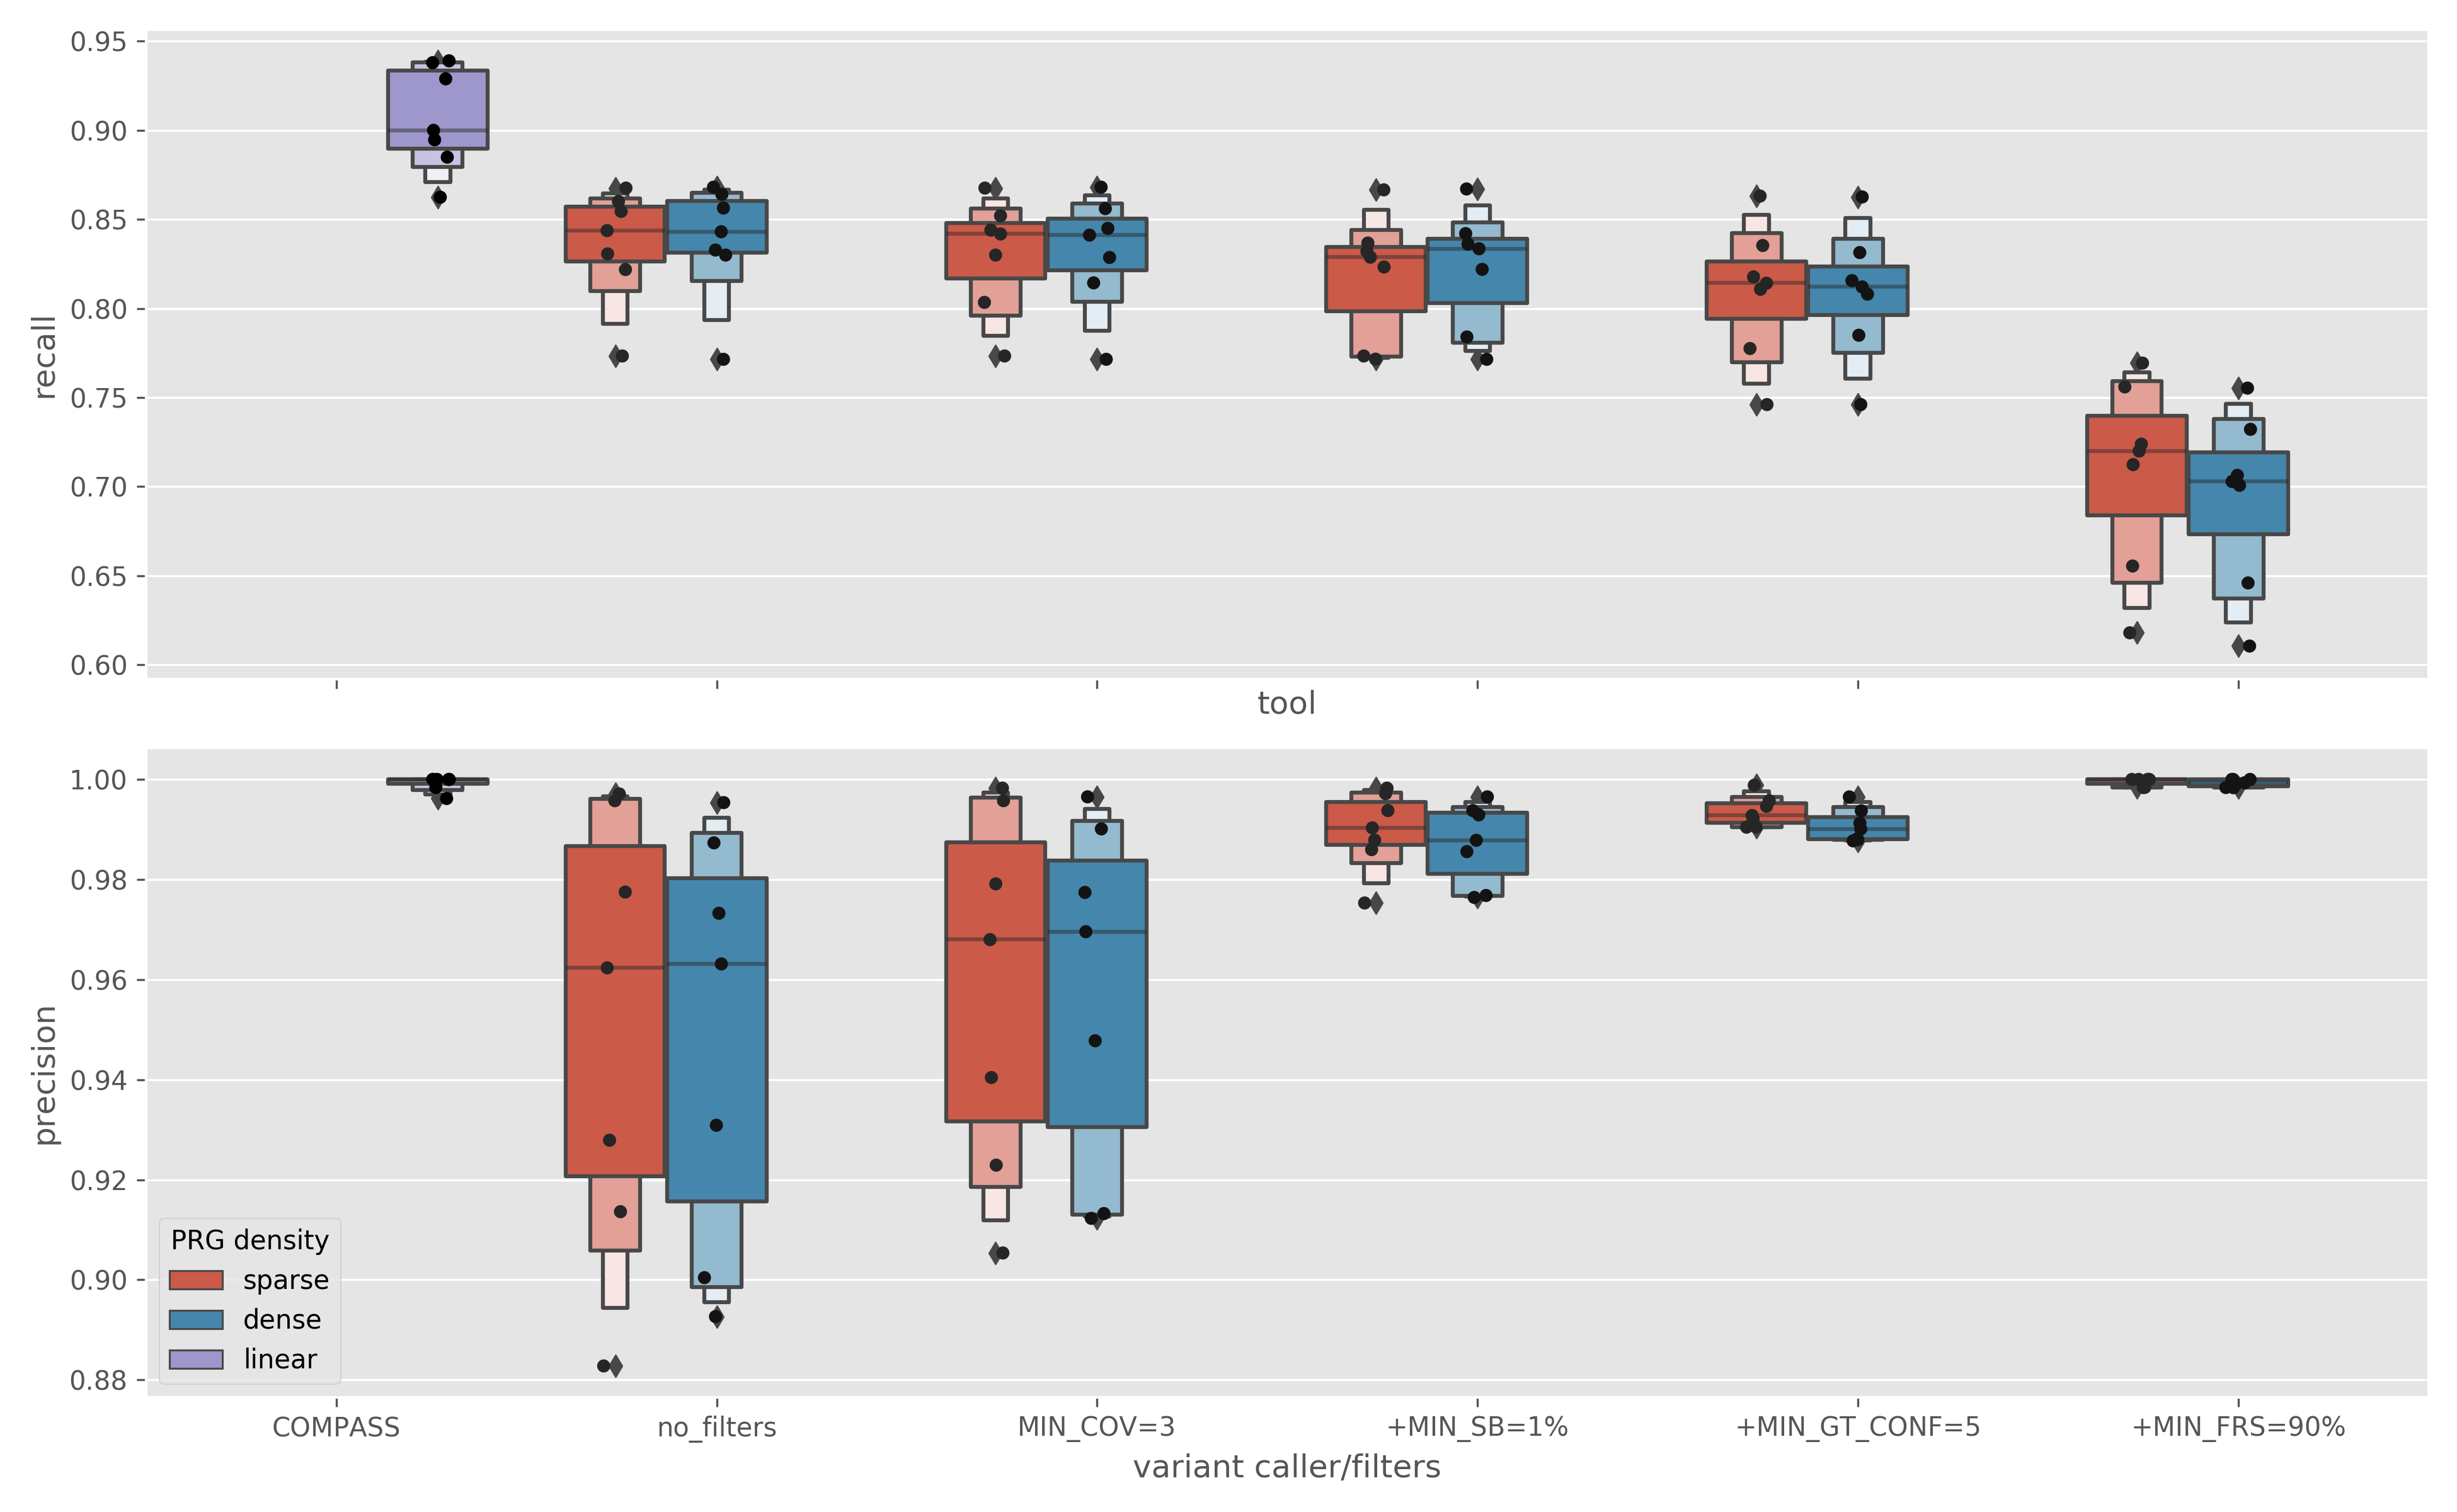
\includegraphics[width=0.90\columnwidth]{Chapter2/Figs/pandora-precision-recall-filters-snps.png}
\caption{{Precision (bottom) and recall (top) of SNPs for COMPASS (purple) and \pandora{} with sparse (red) and dense (blue) \prg{}s. The \pandora{} boxes start with no filters on the left, with each box moving to the right adding a filter to the previous box. The COMPASS box is a reference to the precision and recall of Illumina variant calls. Linear PRG density refers to the fact that COMPASS uses a single, linear reference genome as opposed to \pandora{}, which uses a genome graph. The black points refer to single data points for the seven samples used. MIN\_COV=minimum depth of coverage;MIN\_SB=minimum strand bias;MIN\_GT\_CONF=minimum genotype confidence score;MIN\_FRS=minimum fraction of read support.
{\label{fig:pandora-filters-snps}}%
}}
\end{center}
\end{figure}

\subsubsection{Multi-sample}

\pandora{}'s \vrb{map} routine infers a consensus sequence for a single sample and outputs variant calls with respect to that consensus. However, \pandora{} also has a multi-sample counterpart - the \vrb{compare} command. The \compare{} routine infers a single consensus sequence for \emph{all} samples. It outputs a locus presence/absence matrix, along with a VCF of genotypes for all samples with respect to the consensus sequence \todo{link to ch1 or 2 section describing compare}. As \compare{} was designed for analysing collections of (potentially divergent) samples, we assess its ability to describe \mtb{} transmission clusters. 

The process for calling variants using \compare{} is first to aggregate the novel variants discovered for each sample in \autoref{sec:map-var-calls}. Then, instead of creating an updated \prg{} for each sample, we use the aggregated novel variants to update the MSAs and \prg{}s as in \autoref{sec:map-var-calls}. In the end, we have a \prg{} that has novel variants from all samples contained within it, rather than the \prg{}s used by \pandora{} \vrb{map}, which only have the novel variants for a single sample. Next, we run \vrb{pandora compare} using these updated sparse and dense \prg{}s and filter the resulting VCF as-per \autoref{sec:pandora-filters}.

As a result of its design, it is not possible to provide \compare{} with a reference to base VCF coordinates on (as in \autoref{sec:map-var-calls}). Therefore, we cannot assess the precision and recall for the seven samples as above. We maintain the same filtering strategy as the single-sample approach, however.

\subsection{Computational performance}
\label{sec:var-call-comp-perf}

In addition to the quality of the variant calls, the computational cost of producing them is also important. The CPU time and maximum memory usage for performing the \ont{} variant calling is shown in \autoref{fig:var-comp-perf}. \pandora{}'s performance is broken down into the individual stages, while \bcftools{} is represented by a single job (\vrb{pileup\_nanopore}). The median maximum memory for \bcftools{} was 8.2GB, although the maximum was as high as 58.5GB. This is compared to the highest \pandora{} step - updating the MSAs with novel variants - with a median maximum memory usage of 9.7GB and 13.3GB for the sparse and dense \prg{}s respectively. The highest memory usage for \pandora{} was 18.6GB during the updating of MSAs, nearly 40GB lower than the peak of \bcftools{}. The median CPU time for \bcftools{} was 35129 seconds, or 9.75 hours, with the longest run coming in at 138364 seconds (38.4 hours). To be able to compare \bcftools{} with \pandora{} as a whole, we can sum the median CPU time over each step, which gives 21704 and 53194 seconds, or 6.0 and 14.7 hours, for the sparse and dense \prg{}s respectively. As with the memory usage, the longest runtime component of the \pandora{} pipeline was updating the MSAs with \denovo{} variants. Note, \bcftools{}' \vrb{mpileup} command is not parallelised, while \pandora{}'s steps are, so the wall clock time for the two is dependent on the number of CPU cores available. 

The time and memory of \compare{} is not directly comparable to \bcftools{} and \pandora{} \vrb{map} as it runs on all samples at the same time. Additionally, the novel variant discovery phase of \pandora{} \vrb{map} for all samples technically contributes to the overall runtime of \compare{}. As the performance of this discovery step has already been reported, we outline the remainder of the \compare{} steps in \autoref{tab:compare-perf}. In total, the remainder of the sparse and dense \prg{} steps took 58.4 and 83.1 CPU hours, respectively. The actual wall clock time for these steps was 5.5 and 7.3 hours using 32 CPUs. Maximum memory usage occurred while updating the MSAs and peaked at 38 and 37GB for the sparse and dense \prg{}s, respectively.

\begin{figure}
     \centering
     \begin{subfigure}[b]{0.475\textwidth}
         \centering
         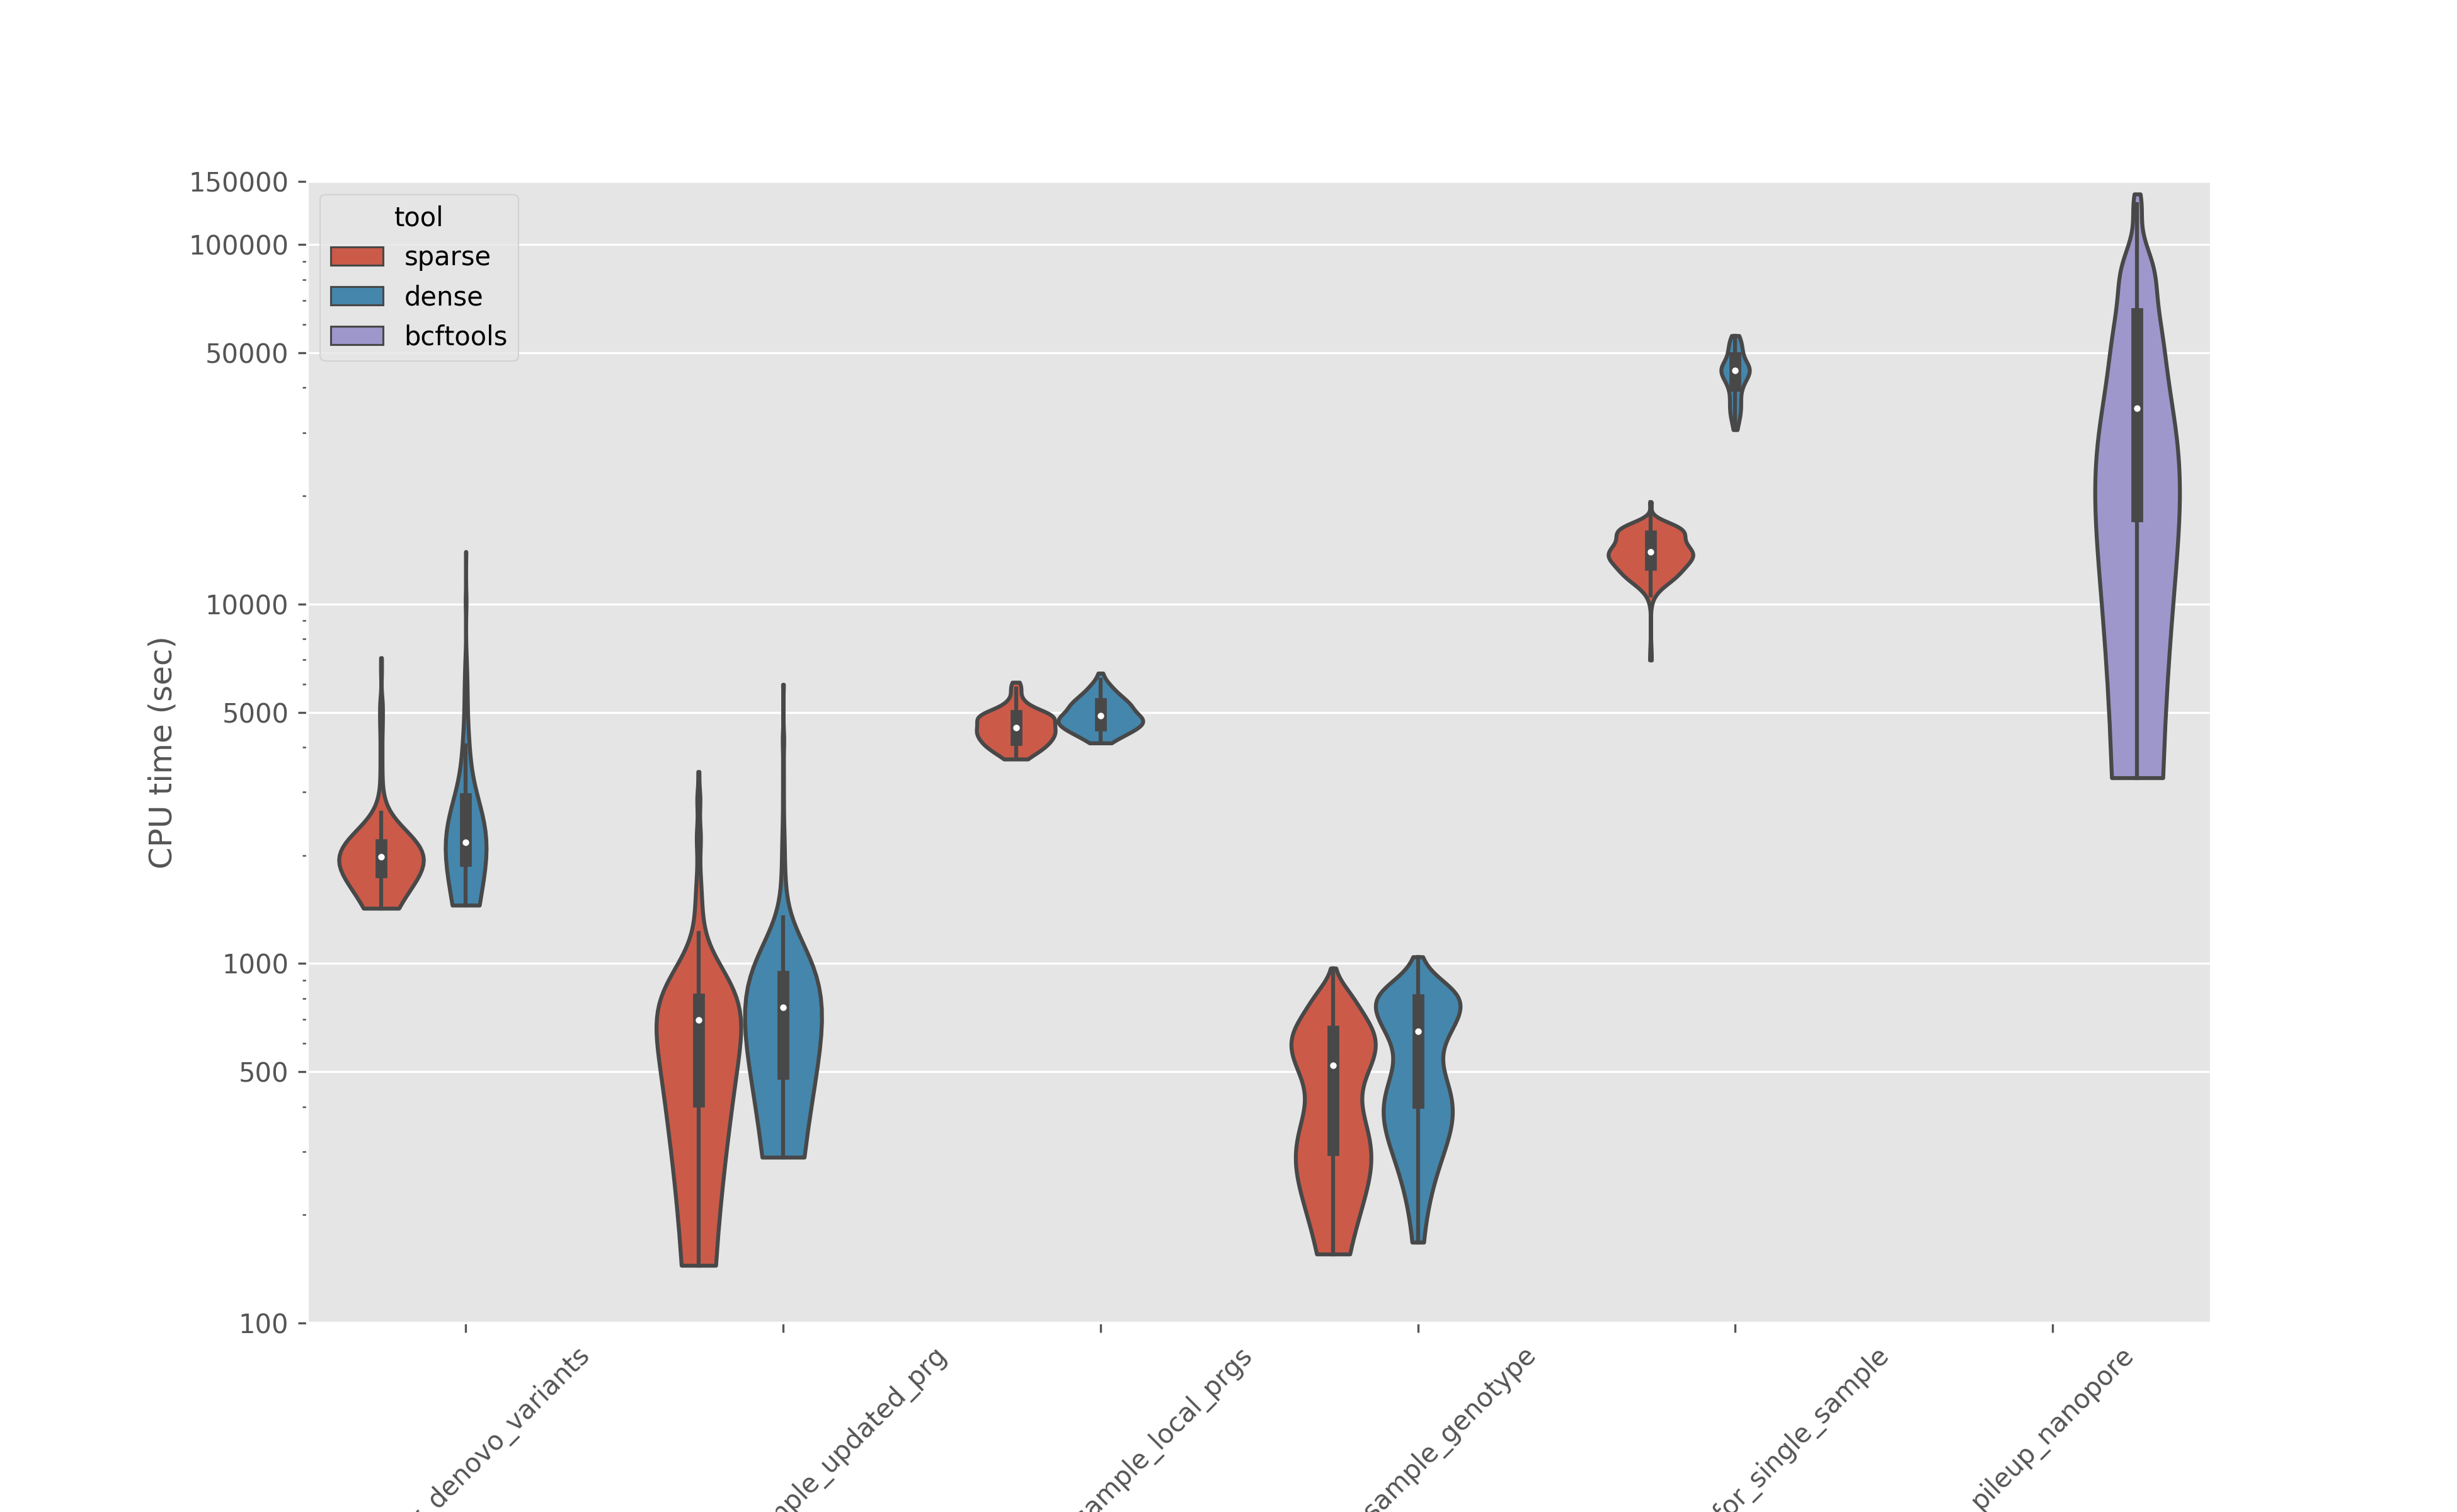
\includegraphics[width=\textwidth]{Chapter2/Figs/cpu_time.png}
         \caption{}
         \label{fig:cpu-time}
     \end{subfigure}
    %  \hfill
     \begin{subfigure}[b]{0.475\textwidth}
         \centering
         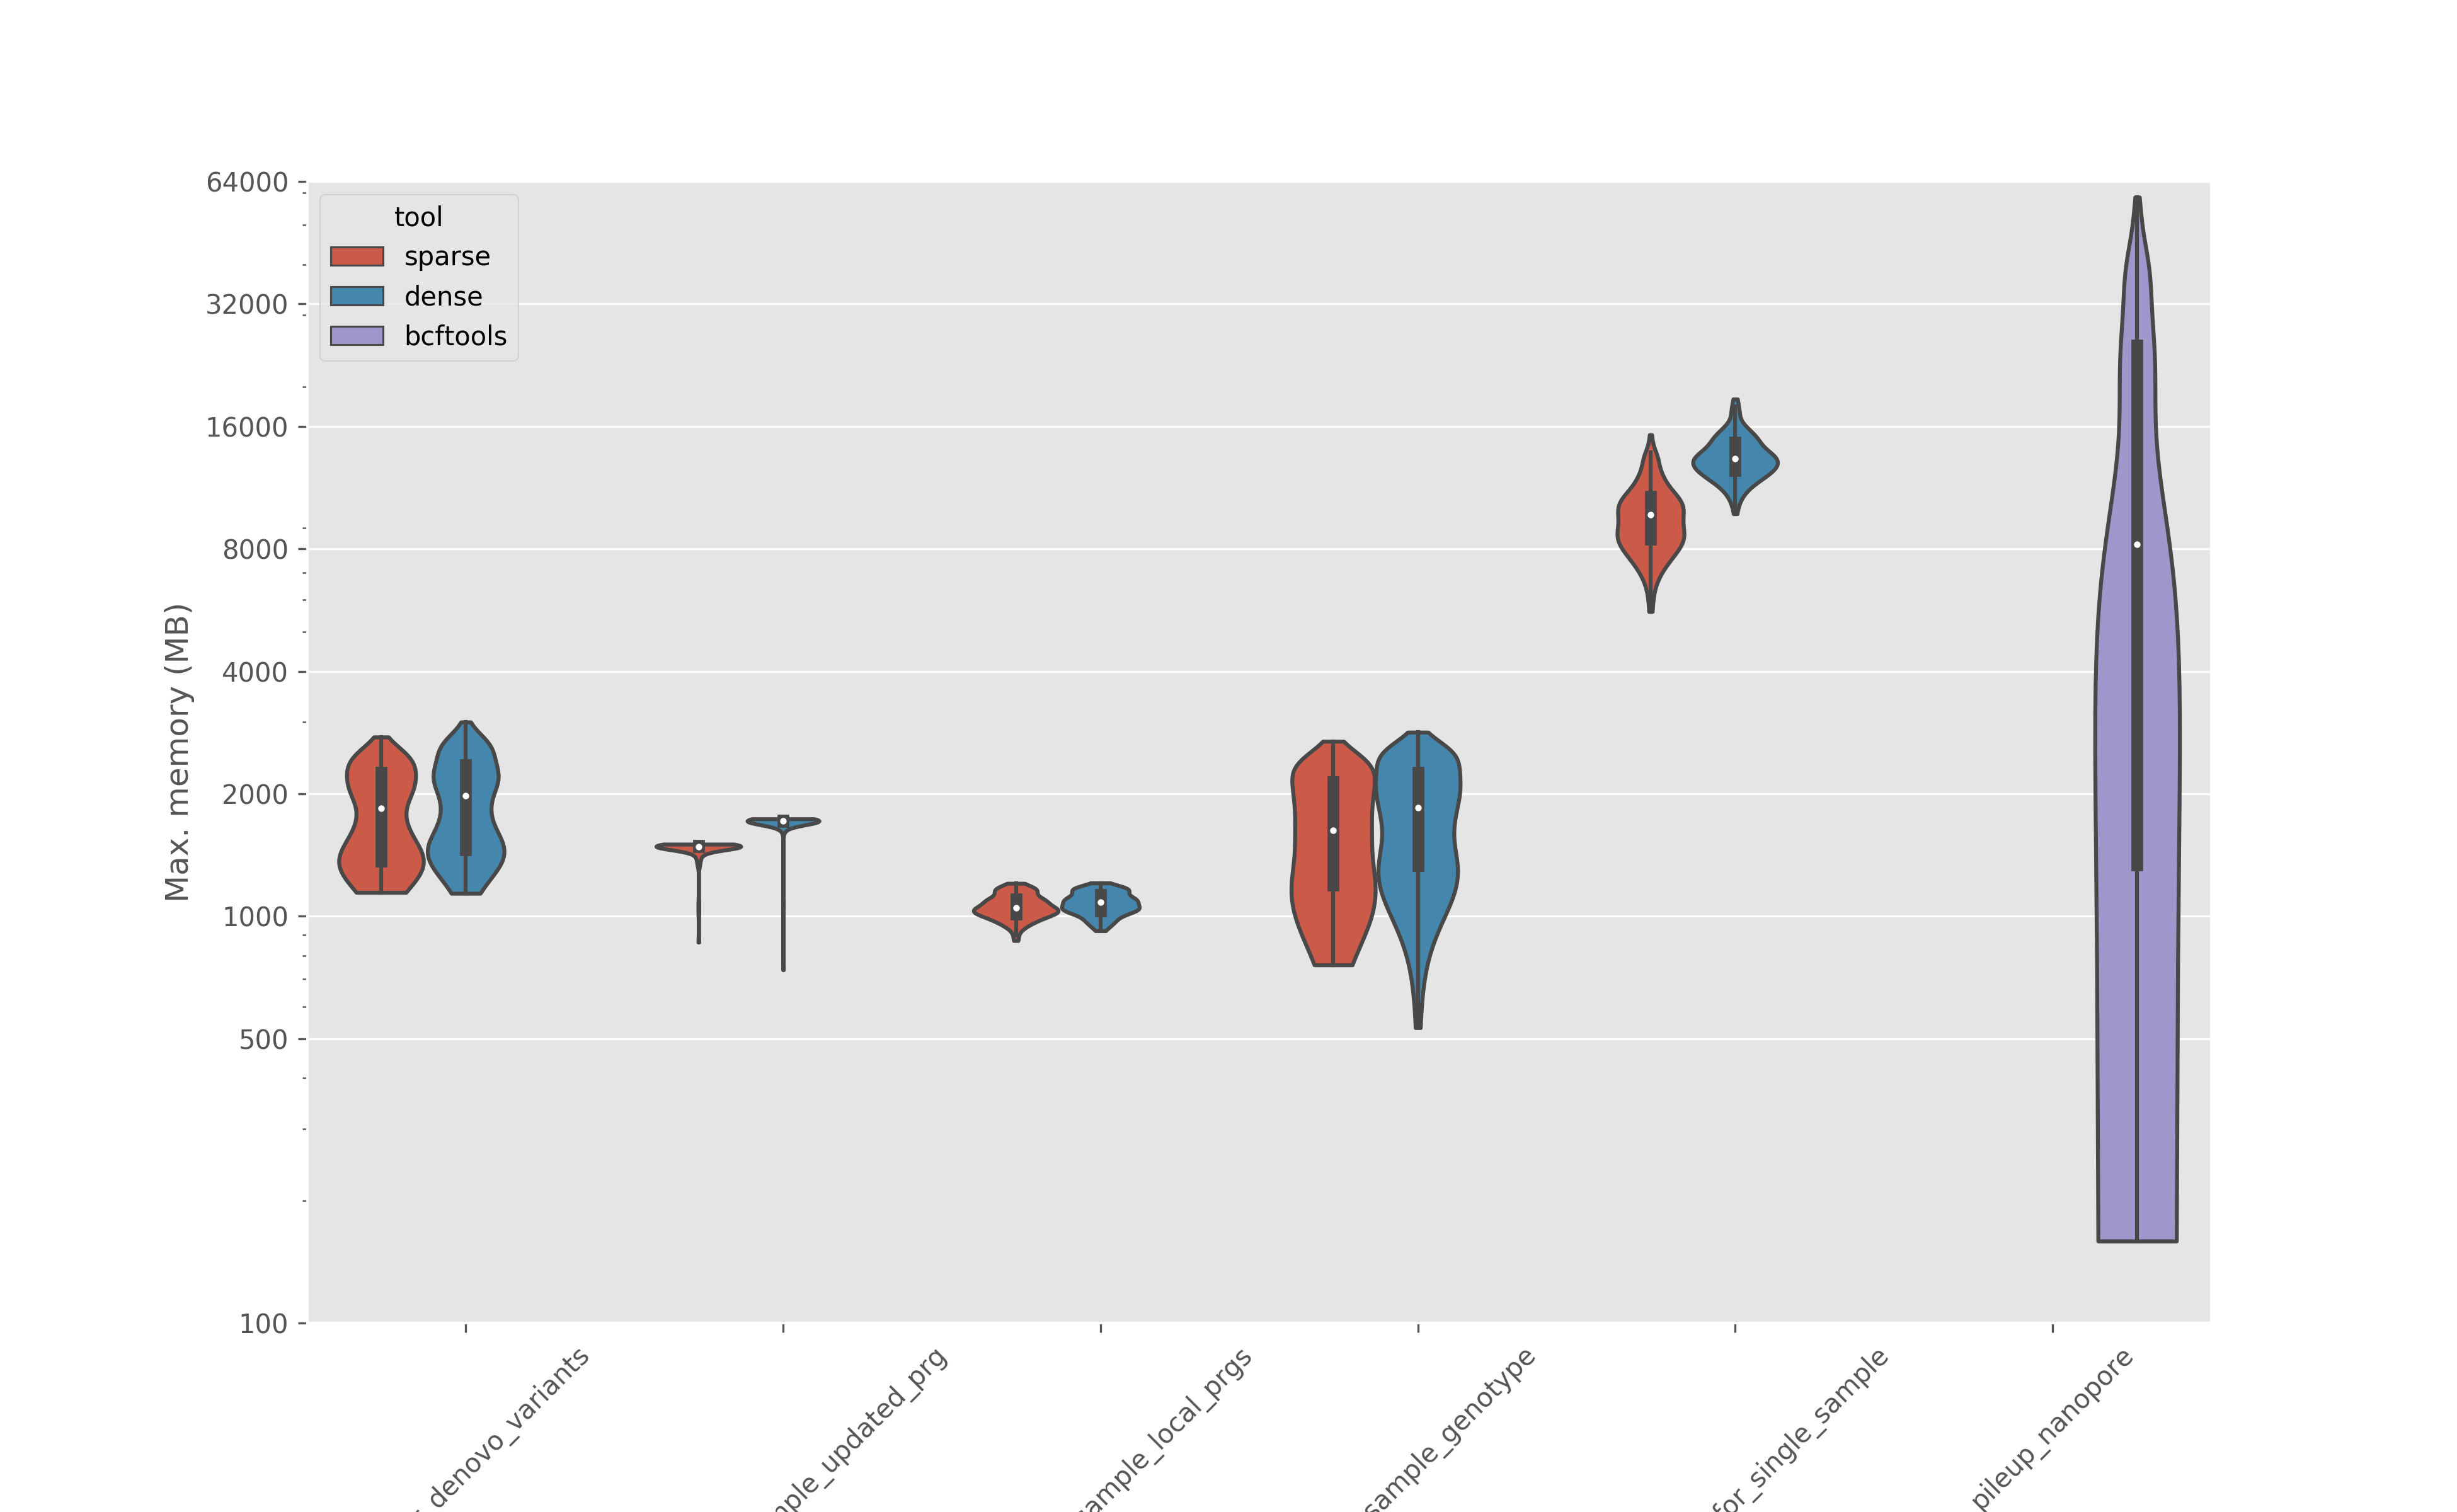
\includegraphics[width=\textwidth]{Chapter2/Figs/max_mem.png}
         \caption{}
         \label{fig:max-mem}
     \end{subfigure}
        \caption{The CPU time (in seconds; y-axis; \textbf{a}) and maximum memory usage (in megabytes; y-axis; \textbf{b}) for each \ont{} variant-calling job. Sparse (red) and dense (blue) refer to \pandora{} steps with the respective density \prg{}. \vrb{bcftools} (purple) only has one step (\vrb{pileup\_nanopore}). The violins represent the distribution of CPU time over all samples.}
        \label{fig:var-comp-perf}
\end{figure}

\begin{table}
\centering
\begin{tabularx}{0.95\textwidth}{|l|Y|Y|Y|Y|Y|Y|}
\hline
                & \multicolumn{3}{c|}{Sparse}                         & \multicolumn{3}{c|}{Dense}                        \\ \hline
Step            & CPU time (sec) & Real time (H:m)  & Max. RAM (GB)   & CPU time (sec) & Real time (H:m)  & Max. RAM (GB) \\ \hline
Update MSA      & 114677         & 1:01             & 38              & 130221         & 1:15             & 37            \\ \hline
Make PRG        & 4700           & 0:05             & 1.2             & 5403           & 0:06             & 1.1           \\ \hline
Index           & 538            & 0:01             & 2.1             & 1224           & 0:02             & 2.4           \\ \hline
Compare         & 90486          & 4:25             & 5.4             & 162294         & 6:04             & 6.1           \\ \hline
\end{tabularx}
\caption{CPU and wall clock time, and memory (RAM) usage for the main steps of running \pandora{}'s multi-sample routine \vrb{compare}. Sparse and Dense refer to two different densities with respect to the number of variants used. All steps were run on a single compute node with 32 CPU cores. MSA=multiple sequence alignment; PRG=population reference graph.}
\label{tab:compare-perf}
\end{table}

\subsection{Summary}
\label{sec:var-summary}

In summary, \autoref{fig:prec-recall-filters} shows that our selection of filters for \ont{} variant callers provides precision on-par with Illumina. However, this precision comes at the cost of a loss in recall. The remainder of this chapter explores how the SNP calls from \ont{} can be used to calculate distances between samples and define putative transmission clusters from these distances. We are especially interested in how similar the pairwise distances are between samples and sequencing modality and whether the same distance thresholds used for Illumina can also be used for \ont{}.

\begin{figure}
\begin{center}
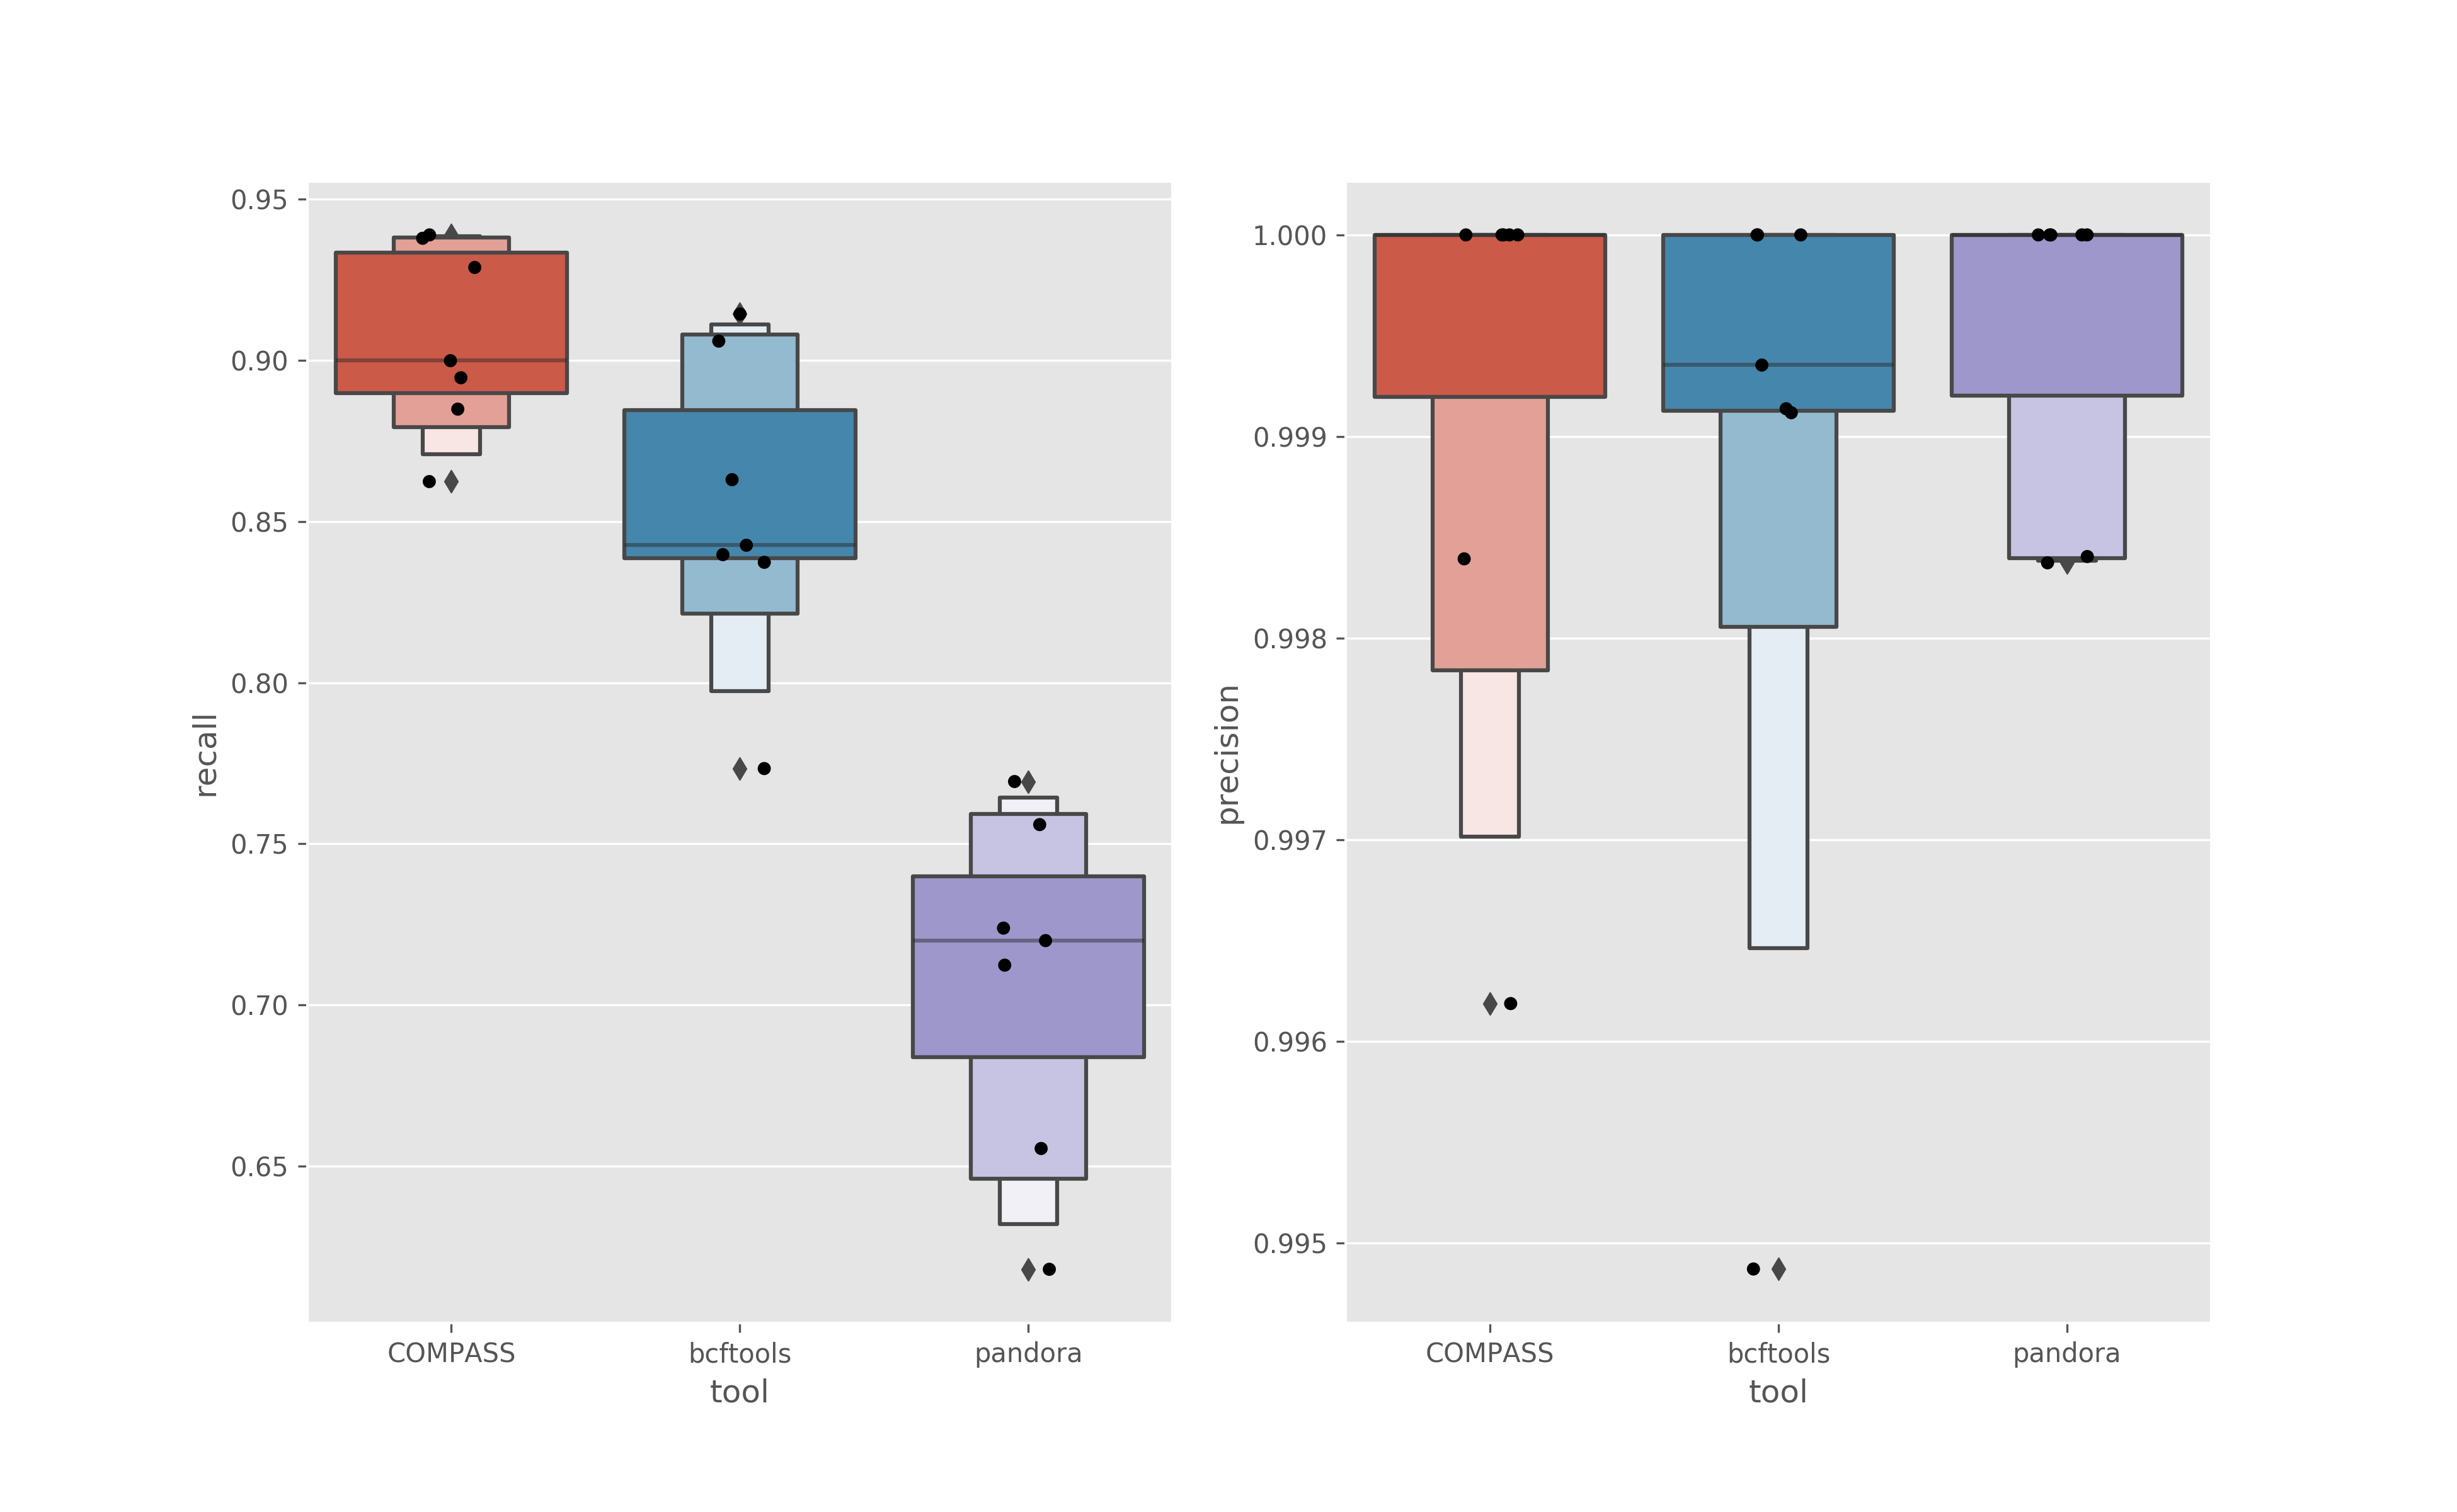
\includegraphics[width=0.9\columnwidth]{Chapter2/Figs/combined-precision-recall-filters-snps.png}
\caption{{Precision (left) and recall (right) of filtered SNPs for COMPASS (red), \bcftools{} (blue), and \pandora{} (purple). Each black point represents one of seven evaluation samples. 
{\label{fig:prec-recall-filters}}%
}}
\end{center}
\end{figure}

%=========================================================================

\section{Pairwise SNP distance comparison}
\label{sec:snp-dist}

When attempting to infer transmission clusters, one approach defines a SNP distance threshold and says that any genomes within this distance of each other are clustered (possible transmissions) \cite{walker2013}. It follows that the SNPs used must be trusted. Having shown we can achieve SNP precision on-par with Illumina using \ont{} data (see \autoref{sec:var-calls}), we investigate the pairwise SNP distance between samples produced by both Illumina and \ont{} sequencing technologies. The intention here is to determine whether the thresholds typically used for Illumina data can also be used for \ont{}, or whether adjustments are required.

To determine the distance between samples, we first generate sample consensus sequences. We do this for each variant-caller: COMPASS (Illumina), \bcftools{} (\ont{}), and \pandora{} \vrb{map} (\ont{}) (not \compare{}). A consensus sequence is obtained by applying the calls from a given VCF (from \autoref{sec:var-calls}) to the \mtb{} reference genome. We nullify (mark as \vrb{N}) any positions where: i) the position failed filtering, ii) the reference genome position does not appear in the VCF file (except for \pandora{} single-sample), iii) the called genotype is null, or iv) the position is within the reference genome mask. 

Next, all sample consensus sequences for a variant-caller are joined into a single FASTA file and a pairwise distance matrix is calculated using \vrb{snp-dists} (version 0.7.0) \cite{snp-dists}. In the case of \compare{} (multi-sample mode), we cannot follow this approach for generating a consensus sequence and distance matrix due to the inability to translate the coordinates from a graph to a linear reference. Instead of a consensus sequence, we generate a genotype array by extracting the called genotype for each sample at each site (VCF entry). Where a site has failed a filter, we use a genotype value of -2. To calculate the distance between two samples, we compare their genotype arrays; if either sample's genotype is $<0$ (i.e., null or filtered) or the genotypes are the same, we record a distance of 0, otherwise 1. The sum of these comparisons for each genotype is the distance between the two samples.

The pairwise SNP distance relationship is presented in \autoref{fig:dotplot}. For a given pair of samples, we plot their SNP distance, based on the COMPASS (Illumina) variant calls (x-axis), against the SNP distance for the same pair, based on the \ont{} variant calls (y-axis). All pairwise comparisons between a sample and itself are absent from the visualisation, and only a single value was used for each pair (i.e., we keep sample1 vs. sample2 and discard sample2 vs. sample1 as they are the same). RANSAC Robust Linear Regression \cite{fischler1981}, as implemented in the Python library \vrb{scikit-learn} \cite{scikitlearn}, was used for determining a linear equation and line-of-best fit for the relationship between pairwise Illumina and \ont{} SNP distance.

If the same thresholds used for Illumina can also be used for \ont{}, we would expect the distances to be the same and the bulk of the points in the plot to fall on the dashed, diagonal identity line in \autoref{fig:dotplot}. What we see instead is a linear relationship that falls \emph{under} this identity line - for all \ont{} variant callers. Given the filtered \ont{} SNP calls made by \bcftools{} and \pandora{} have lower recall than Illumina (\autoref{sec:var-summary}), this is expected, as they miss some SNPs found by Illumina.

We highlight one important observation in the zoomed inset of \autoref{fig:dotplot}. As SNP thresholds used for \mtb{} are generally well below 100 \cite{stimson2019}, it makes more sense to base SNP distance relationships on those samples that are "close". And indeed, when we zoom in on pairs of samples within 100 (Illumina) SNPs of each other, we see an association that is closer to the identity line. Fitting a linear model to this close subset of pairwise distances yields a relationship defined by the equation $y=0.806x+0.593$ for \bcftools{}, $y=0.575x+13.544$ for \pandora{} \vrb{map}, and $y=0.342x+0.765$ for \compare{}. Replacing $x$ with an Illumina SNP threshold gives the (predicted) equivalent \ont{} SNP threshold based on these relationships. For example, at an Illumina SNP distance of 12, the linear equation would predict a corresponding \bcftools{} \ont{} SNP distance of 10.

\begin{figure}
\begin{center}
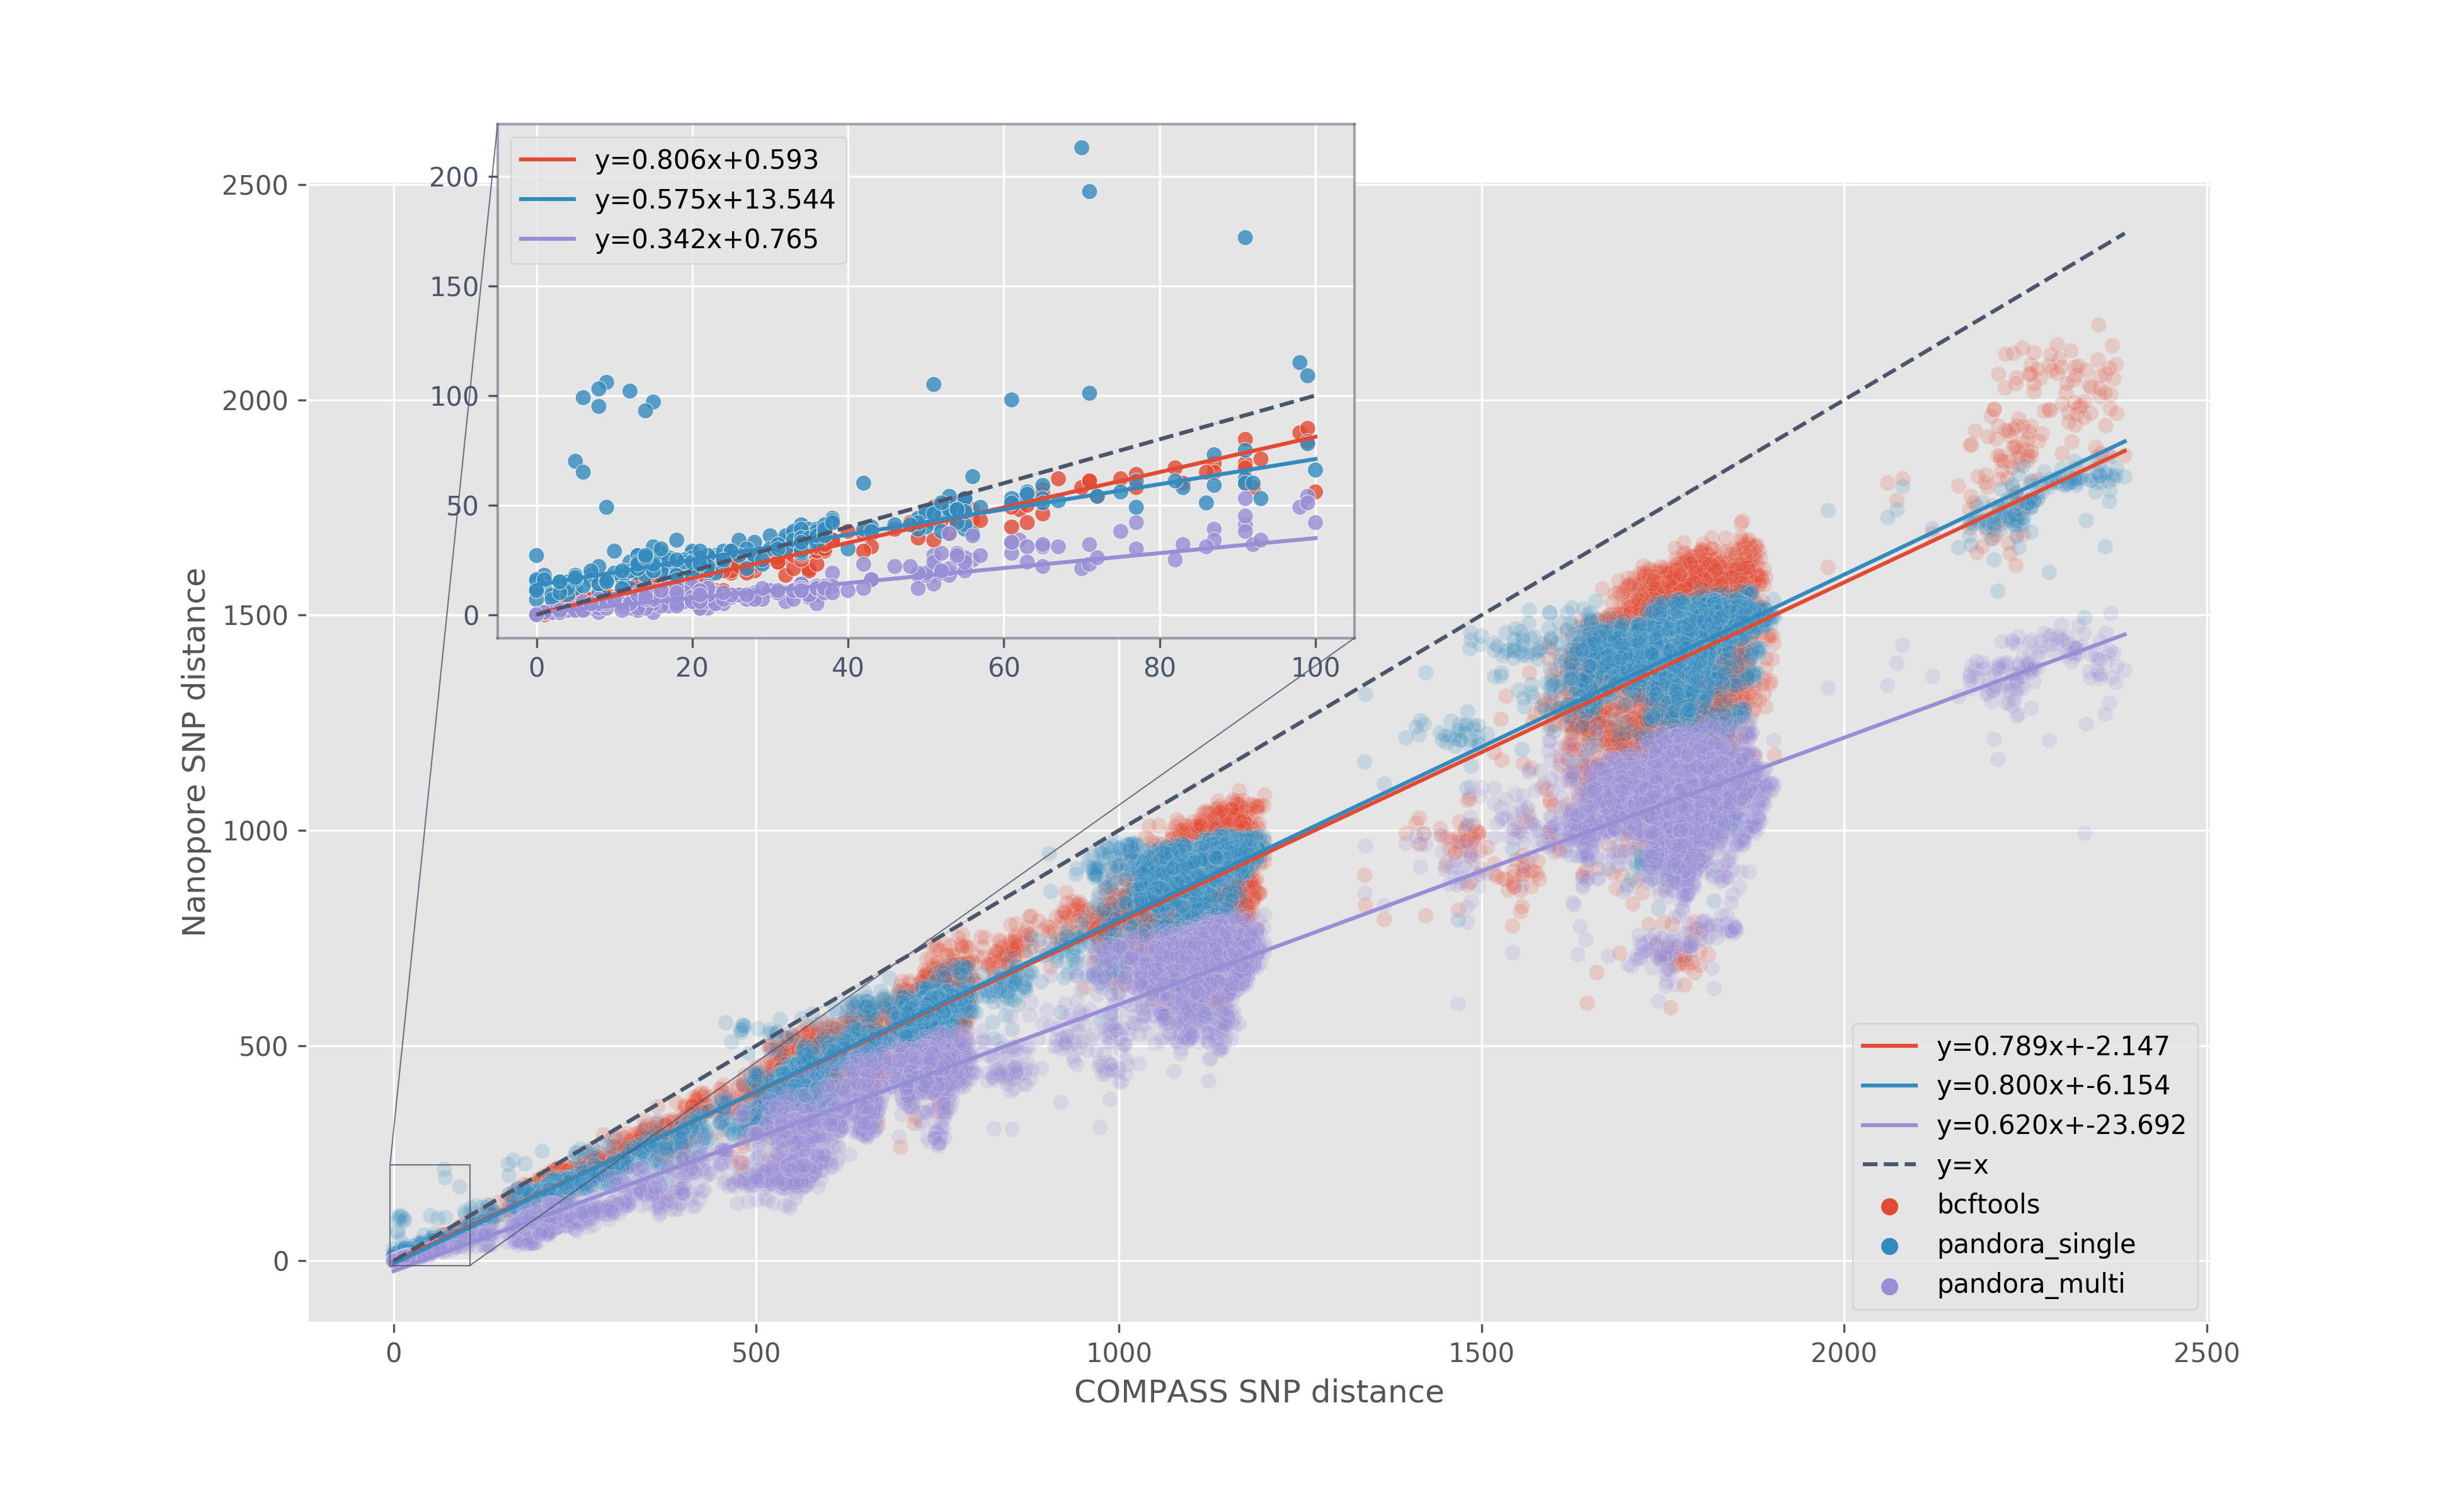
\includegraphics[width=0.90\columnwidth]{Chapter2/Figs/combined-dotplots.png}
\caption{{Pairwise SNP distance relationship between Illumina (COMPASS; x-axis) and \ont{} (\bcftools{} (red), and \pandora{} single-sample (blue) and multi-sample (purple) mode; y-axis) data. Each point represents the SNP distance between two samples for the two sequencing modalities. The black, dashed line shows the identity line (i.e. $y=x$) and the coloured lines shows the line of best fit based on the robust linear model fit to the data. The zoomed inset shows all pairs where the COMPASS distance is $\le 100$.
{\label{fig:dotplot}}
}}
\end{center}
\end{figure}

%  see https://github.com/mbhall88/head_to_head_pipeline/issues/61 for a full investigation of the outliers discussed below
In the middle-left of the inset in \autoref{fig:dotplot} a small cluster of \pandora{} \vrb{map} (blue) points can be seen. These have an approximate pairwise \ont{} distance of 100, but \texttildelow10 for Illumina. Upon further investigation, the cause of the large discrepancy in the distance was due to \pandora{} \vrb{map} failing to identify (and filter) some heterozygous calls. Two samples, in particular, occur as one member in all of the major outlying pairs. 94\% of the false-positive differences leading to the large \ont{} distances occur at positions that are filtered due to evidence of heterozygosity in COMPASS. That is, in the Illumina consensus sequence, these positions are ignored due to filtering and do not count as a difference. However, \pandora{} did not have sufficient read depth on both alleles to trigger the FRS filter (\autoref{sec:pandora-filters}) - leading to a passing variant call that differs from the sample it is being compared with. 

\noindent
The relationship between Illumina and \ont{} distances is indeed linear for all three variant-calling methodologies. While the relationship is not identical, we will attempt to use linear models fit to the relationship to infer what \ont{} SNP distance threshold is likely to align with a given Illumina threshold for defining putative transmission clusters.

%=========================================================================

\section{\ont{} transmission clustering}
\label{sec:clustering}

While the relationship between Illumina and \ont{} pairwise SNP distance is enlightening, ultimately, the fundamental question is: do \ont{} SNPs lead to transmission clusters consistent with those obtained with Illumina SNPs? To answer this question, we compare Illumina- and \ont{}-based clusters for four Illumina SNP thresholds. 

Selecting a SNP threshold to infer transmission clusters from has seen a variety of values recommended \cite{stimson2019}. As we seek to show concordance of \ont{} data with PHE's Illumina-based strategy, we opt to investigate Illumina threshold values 0, 2, 5, and 12. PHE define two cases as clustered if they have a SNP distance $\le 12$ as "\emph{12 SNPs represents the maximum SNP difference between 2 isolates for which epidemiological links have previously been identified \cite{walker2013} and is a conservative measure for reporting isolate relatedness}" \cite{phe-tb-england}. Five was likewise selected as Walker \etal{} \cite{walker2013} found it to indicate membership in a recent transmission chain. Finally, threshold values 0 and 2 were chosen to provide insight into the level of granularity possible and are of clinical interest in some settings (personal correspondence with Tim Peto). For each of these four thresholds, we investigate what corresponding \ont{} SNP distance threshold yields the most similar clustering.

\subsection{Transmission cluster similarity}
\label{sec:cluster-similarity}

We use the distance matrices from \autoref{sec:snp-dist} to infer transmission clusters. To cluster samples, for a given SNP threshold $t$, we use pairs of samples with a distance $\le t$ to define a graph, $G=(V,E)$, where samples (nodes, $V$) are connected by weighted edges ($E$), with the weight of an edge indicating the distance between the two samples it connects. We define clusters as the set of connected components $\{C_1, C_2...C_N\}\in G$, where $N$ is the number of clusters. That is, a cluster (connected component), $C_i$, is a subgraph of $G$ where a path exists between any two samples in $C_i$, but no path exists to any samples in the rest of $G$. With this definition, all clusters have a minimum of two members. 

To assess how closely \ont{} SNP-based clustering approximates Illumina SNP-based clustering, we adapt a similarity measure on sets; the Tversky Index \cite{tversky1977}. We define the Illumina clustering as $G$ and the \ont{} clustering as $H$. We are interested in being able to quantify the recall and precision of the \ont{} clustering with respect to Illumina. In this sense, recall describes when clustered samples in $G$ are not clustered (or are in the wrong cluster) in $H$. Likewise, precision in this context tells us when extra samples are added to existing clusters by $H$ or when clusters in $G$ are joined in $H$. 

In order to be able to define precision and recall when comparing two clustering graphs $G$ and $H$, we define the Tversky Index

\begin{equation}
\label{eq:tversky-index}
   TI(n, G, H)=\frac{\left|C_{n,G}\cap C_{n,H}\right|}{\left|C_{n,G}\cap C_{n,H}\right|+\alpha |C_{n,G}-C_{n,H}|+\beta |C_{n,H}-C_{n,G}|}
\end{equation}

where $C_{n,G}$ is the cluster in $G$ that sample $n$ is a member of. When $\alpha = 1$ and $\beta=0$ in \autoref{eq:tversky-index}, we get a metric analogous to recall - as described above. Therefore, we define recall, $R$, for a single sample $n$ as

\begin{equation}
\label{eq:recall}
   R(n, G, H)=\frac{\left|C_{n,G}\cap C_{n,H}\right|}{\left|C_{n,G}\cap C_{n,H}\right|+|C_{n,G}-C_{n,H}|}=\frac{\left|C_{n,G}\cap C_{n,H}\right|}{|C_{n,G}|}
\end{equation}

When $\alpha = 0$ and $\beta = 1$ in \autoref{eq:tversky-index}, we get a metric analogous to precision. As such, we define precision $P$, for a single sample $n$ as

\begin{equation}
\label{eq:precision}
   P(n, G, H)=\frac{\left|C_{n,G}\cap C_{n,H}\right|}{\left|C_{n,G}\cap C_{n,H}\right|+|C_{n,H}-C_{n,G}|}=\frac{\left|C_{n,G}\cap C_{n,H}\right|}{|C_{n,H}|}
\end{equation}

With these definitions for a single sample, we can assess the recall and precision of the \ont{} clustering, $H$, with respect to the Illumina clustering, $G$, by averaging each metric over all samples in $G$. This gives us the Sample-Averaged Cluster Recall (SACR)

\begin{equation}
\label{eq:sacr}
   SACR=\frac{\sum_{n}^{V_G}R(n, G, H)}{|V_G|}
\end{equation}

where $V_G$ is the set of samples (nodes) in $G$ (Illumina graph). Likewise, we define the Sample-Averaged Cluster Precision (SACP) as 

\begin{equation}
\label{eq:sacp}
   SACP=\frac{\sum_{n}^{V_G}P(n, G, H)}{|V_G|}
\end{equation}

SACR states, on average, what proportion of the samples clustered together in $G$ are also clustered together in $H$ (\ont{}) - it is a measure of how many true positives \ont{} retains. Inversely, SACP states, on average, what proportion of the samples clustered together in $H$ are also clustered together in $G$ - it is a measure of how many extra samples \ont{} adds to clusters. 

However, SACR and SACP do not inherently account for when $H$ has clusters containing only samples deemed non-clustered (singleton) in $G$. In order to quantify any extra clustering by $H$, we establish the Excess Clustering Rate (XCR) as the proportion of singletons (disconnected nodes) in $G$ that are connected in $H$. We define XCR as

\begin{equation}
\label{eq:xcr}
    XCR = \frac{|S_G-S_H|}{|S_G|}
\end{equation}

where $S_G$ and $S_H$ are the sets of singletons in the respective graphs. 

\noindent
We assess the cluster similarities using the Python programming language with the \vrb{networkx} library \cite{networkx}. For a given threshold, we create the Illumina clustering (graph), $G$, and the \ont{} clustering, $H$ - as described above - and use these to calculate the SACR, SACP, and XCR using \autoref{eq:sacr}, \autoref{eq:sacp}, and \autoref{eq:xcr} respectively.

\subsubsection{Summary}

To summarise, for each sample in an Illumina-defined cluster, SACR is the proportion of samples in its Illumina cluster also in its \ont{} cluster - averaged over all samples. SACP is the proportion of samples in its \ont{} cluster also in its Illumina cluster - averaged over all samples. SACR indicates whether samples have been missed from \ont{} clustering (false negatives), and SACP reveals if additional samples are being added to \ont{} clusters (false positives). One shortcoming of SACR and SACP is that they do not account for when the \ont{} clustering contains clusters where no member of the cluster is part of an Illumina cluster. To that end, XCR is the proportion of Illumina non-clustered (singleton) samples added to a cluster by \ont{}. For example, an XCR value of 0.1 would indicate that 10\% of non-clustered samples were part of a cluster in the \ont{} clustering. We provide an illustrated, worked example of these metrics in \autoref{app:cluster-example}.

Of the metrics outlined above, our primary focus is SACR, as samples missed from clusters are of particular concern for public health agencies.

\subsection{Evaluation of transmission clusters}
\label{sec:eval-clusters}

\subsubsection{BCFtools}
\label{sec:bcftools-clustering}

For the four Illumina SNP distance thresholds of interest - 0, 2, 5, and 12 - the corresponding \bcftools{} thresholds we use are 0, 2, 5, and 11. We chose to forego the model-based predicted thresholds and instead use the hand-picked ones based on a threshold parameter-sweep outlined in \autoref{app:dist-sweep}.

\autoref{fig:bcftools-clusters} is a visualisation of these clustering results for \bcftools{}. The graphs depict the true (Illumina/COMPASS) clusters for each SNP threshold. The inner and outer colours of each node represent the SACR and SACP values, respectively, for its cluster. The actual clustering produced by \bcftools{} - without any annotations - can be see in \autoref{fig:bcftools-original-clusters}.

The \bcftools{} clustering results are summarised in \autoref{tab:bcftools-cluster-summary} for all four SNP thresholds analysed. Of note, \bcftools{} achieves a SACR of 1.0 at all thresholds - meaning \ont{} does not miss any samples from their correct clustering. At the SNP threshold of 2, \bcftools{} clustering only differed from Illumina by the addition of one sample to a cluster of three.  SNP threshold 5 had the highest XCR (0.057), due to two new clusters of size 2 and 3, and the addition of 2 singleton samples to a cluster of 5.  The lowest SACP was at threshold 12 due to the additions of two clusters of size two to a larger cluster and three singletons to existing clusters. 

\begin{figure}
\begin{center}
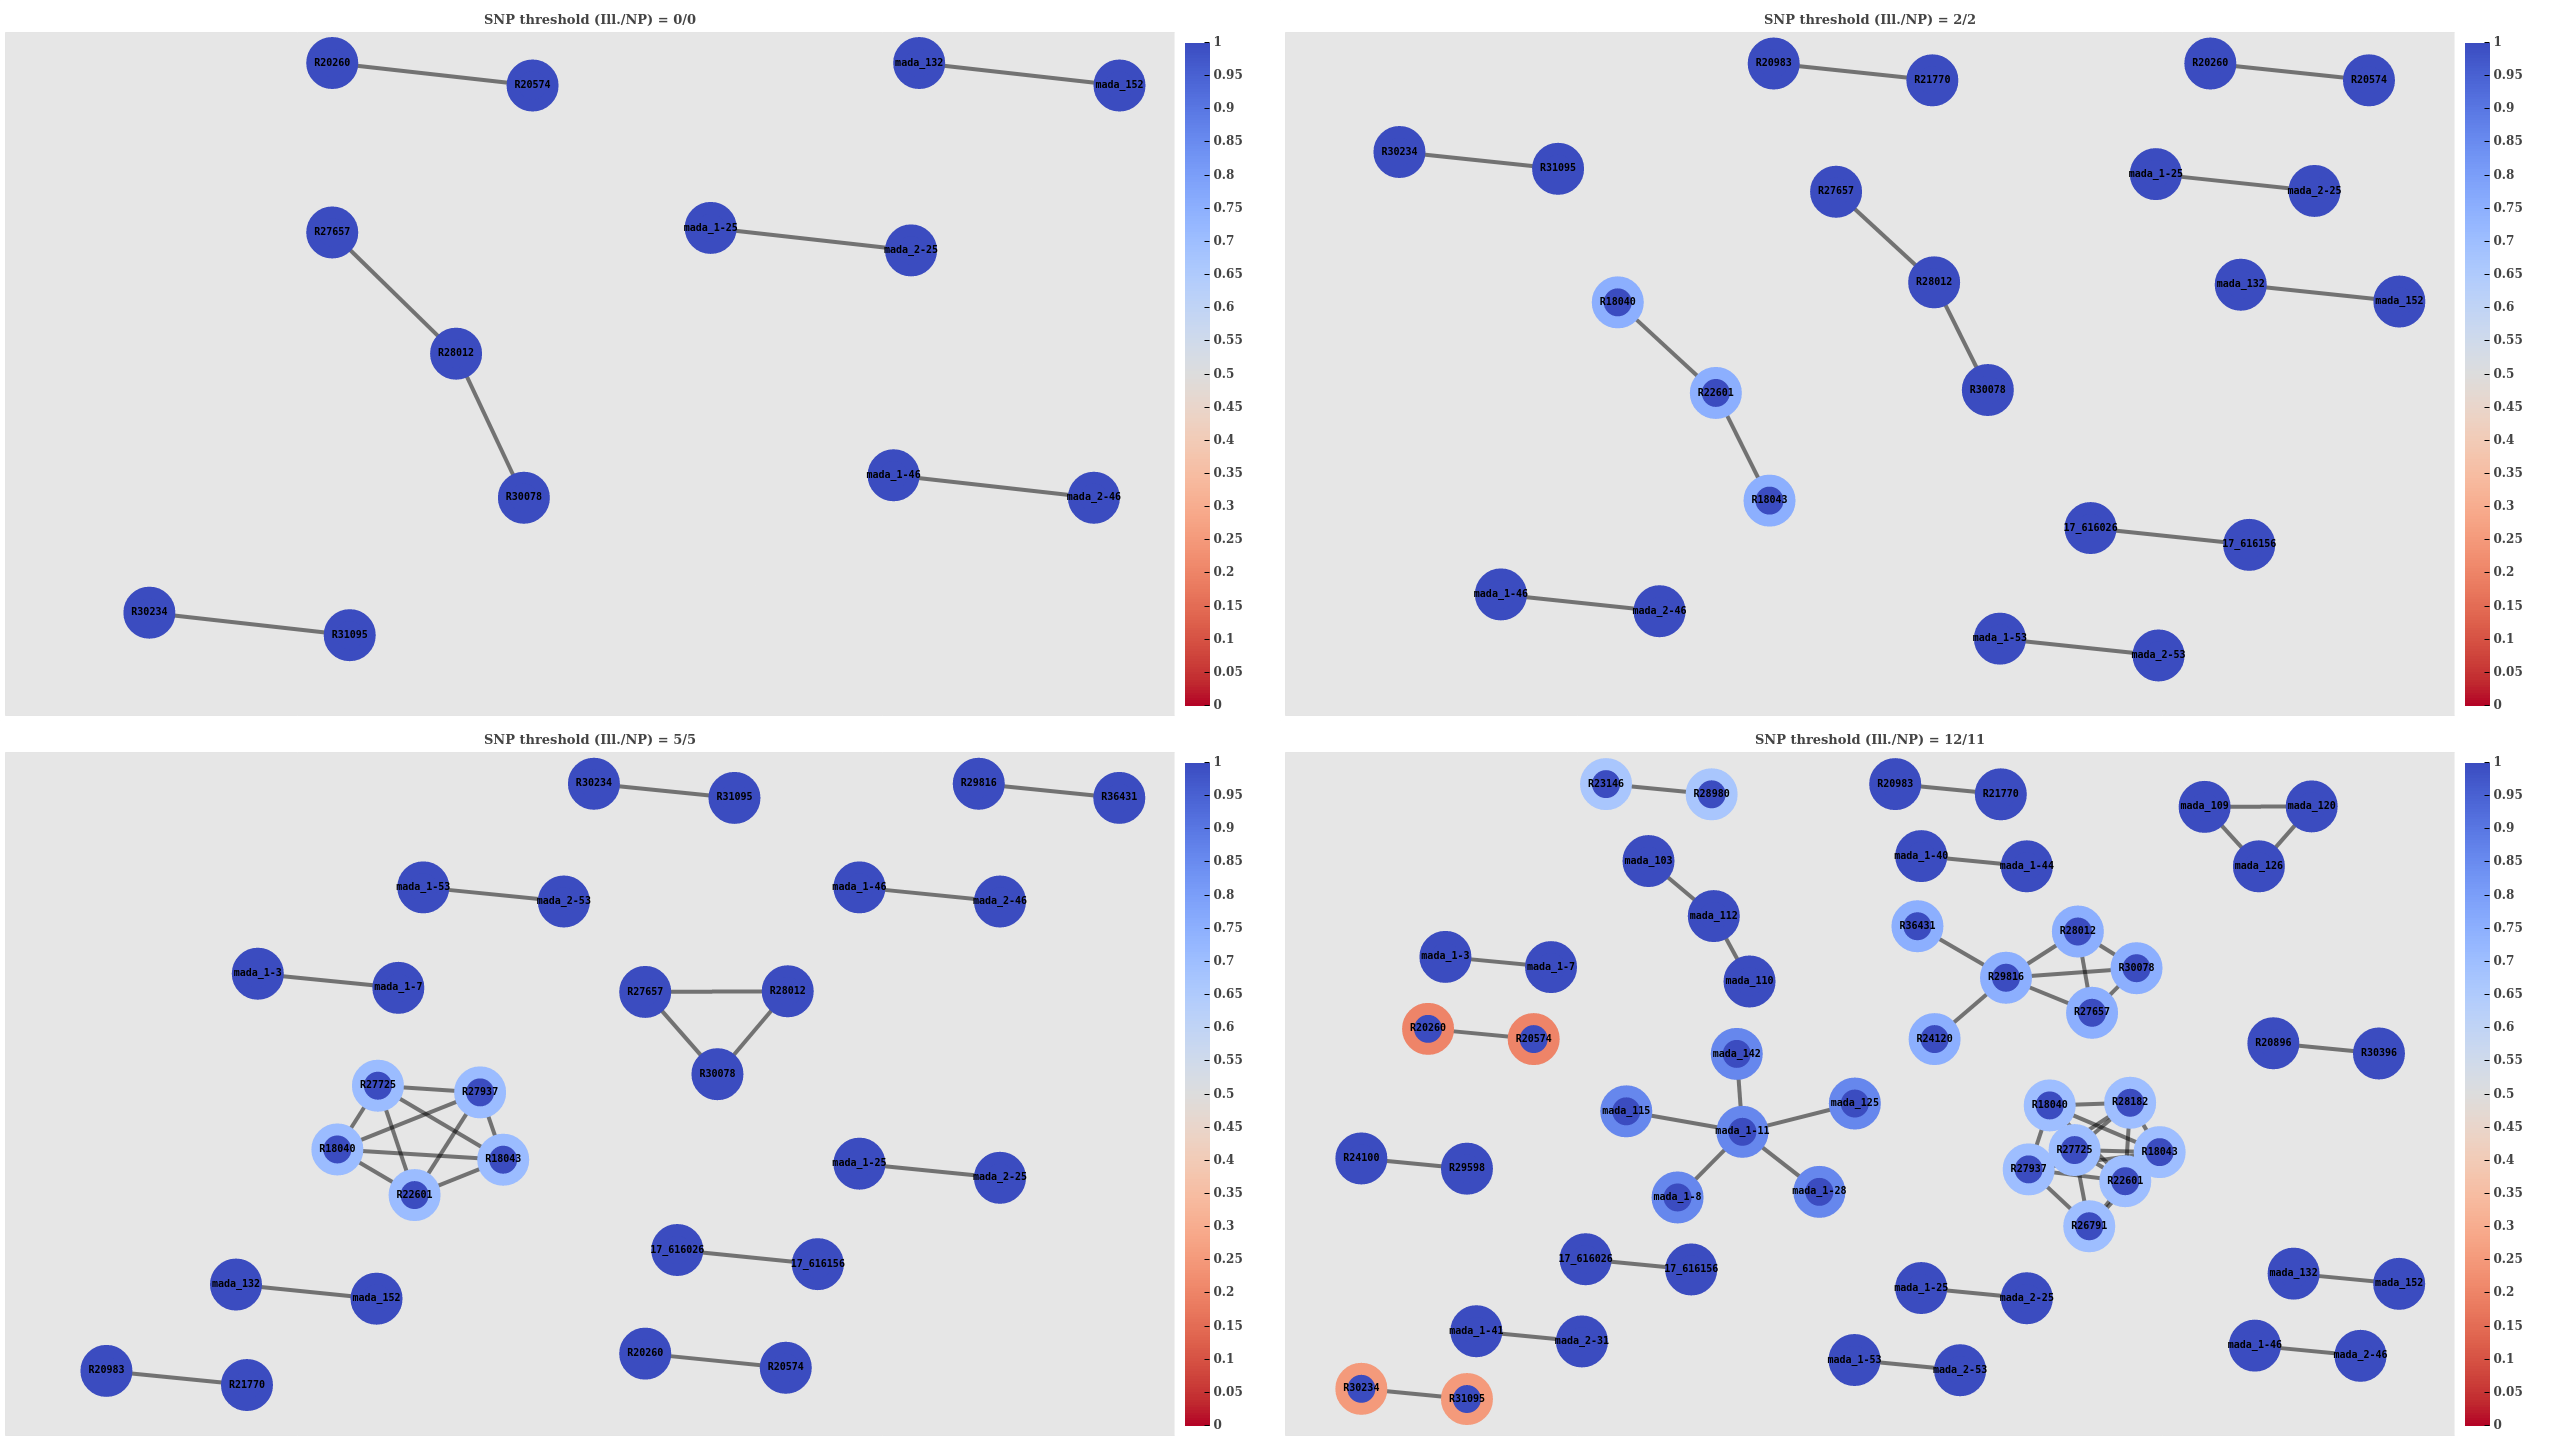
\includegraphics[width=0.90\columnwidth]{Chapter2/Figs/bcftools_clusters.png}
\caption{{Agreement of Illumina and \bcftools{} (\ont{}) transmission clustering at SNP thresholds 0 (top-left), 2 (top-right), 5 (bottom-left) and 12 (bottom-right). The title of each subplot indicates the Illumina (Ill.) and \ont{} (NP) threshold used when clustering. Samples (nodes) are connected when the SNP distance between them is less than or equal to the relevant threshold. The inner and outer colours for each node indicates the SACR and SACP values, respectively, for its cluster. The Illumina-based clustering is shown.
{\label{fig:bcftools-clusters}}
}}
\end{center}
\end{figure}

\begin{table}
\centering
\begin{tabularx}{0.95\textwidth}{|Y|Y|Y|Y|} \hline
Threshold & SACR & SACP  & XCR           \\ \hline
0         & 1.0  & 1.0   & 0.015 (2/137) \\ \hline
2         & 1.0  & 0.966 & 0.008 (1/128) \\ \hline
5         & 1.0  & 0.949 & 0.057 (7/122) \\ \hline
12 (11)   & 1.0  & 0.845 & 0.031 (3/97) \\ \hline
\end{tabularx}
\caption{Summary of \bcftools{} clustering metrics for four (Illumina) SNP distance thresholds. The threshold(s) in parentheses are the \ont{} equivalent threshold used. The fractions in parentheses for XCR indicate the underlying numbers. SACR=sample-averaged cluster recall; SACP=sample-averaged cluster precision; XCR=excess clustering rate.}
\label{tab:bcftools-cluster-summary}
\end{table}

\subsubsection{Pandora single-sample}

For \pandora{} single-sample (\vrb{map}), we also chose to use the hand-picked SNP distance thresholds from analysis in \autoref{app:dist-sweep}. These are 16, 18, 18, and 27 for the Illumina thresholds of interest 0, 2, 5, and 12, respectively. The clustering results for each of these thresholds are summarised in \autoref{tab:map-cluster-summary} and visualised in \autoref{fig:map-clusters}. 

At no threshold was \pandora{} \vrb{} clustering able to achieve perfect SACR, SACP or XCR. In particular, all thresholds had an SACP value less than 0.69 and an XCR greater than 0.11. These results outline the fact that many singletons were erroneously clustered, and many clusters merged. In large part, this is expected due to the much wider spread of distances along the y-axis, in the inset of \autoref{fig:dotplot},  when comparing \pandora{} \vrb{map} to \bcftools{} or \pandora{} multi-sample. Although the SACR values are not as low as the SACP, we place a higher value on them. The nodes with red(ish) inner circles in \autoref{fig:map-clusters} highlight clusters where samples were missed. The actual clusters generated by \pandora{} \vrb{map} can be seen in \autoref{fig:map-original-clusters}.

\begin{figure}
\begin{center}
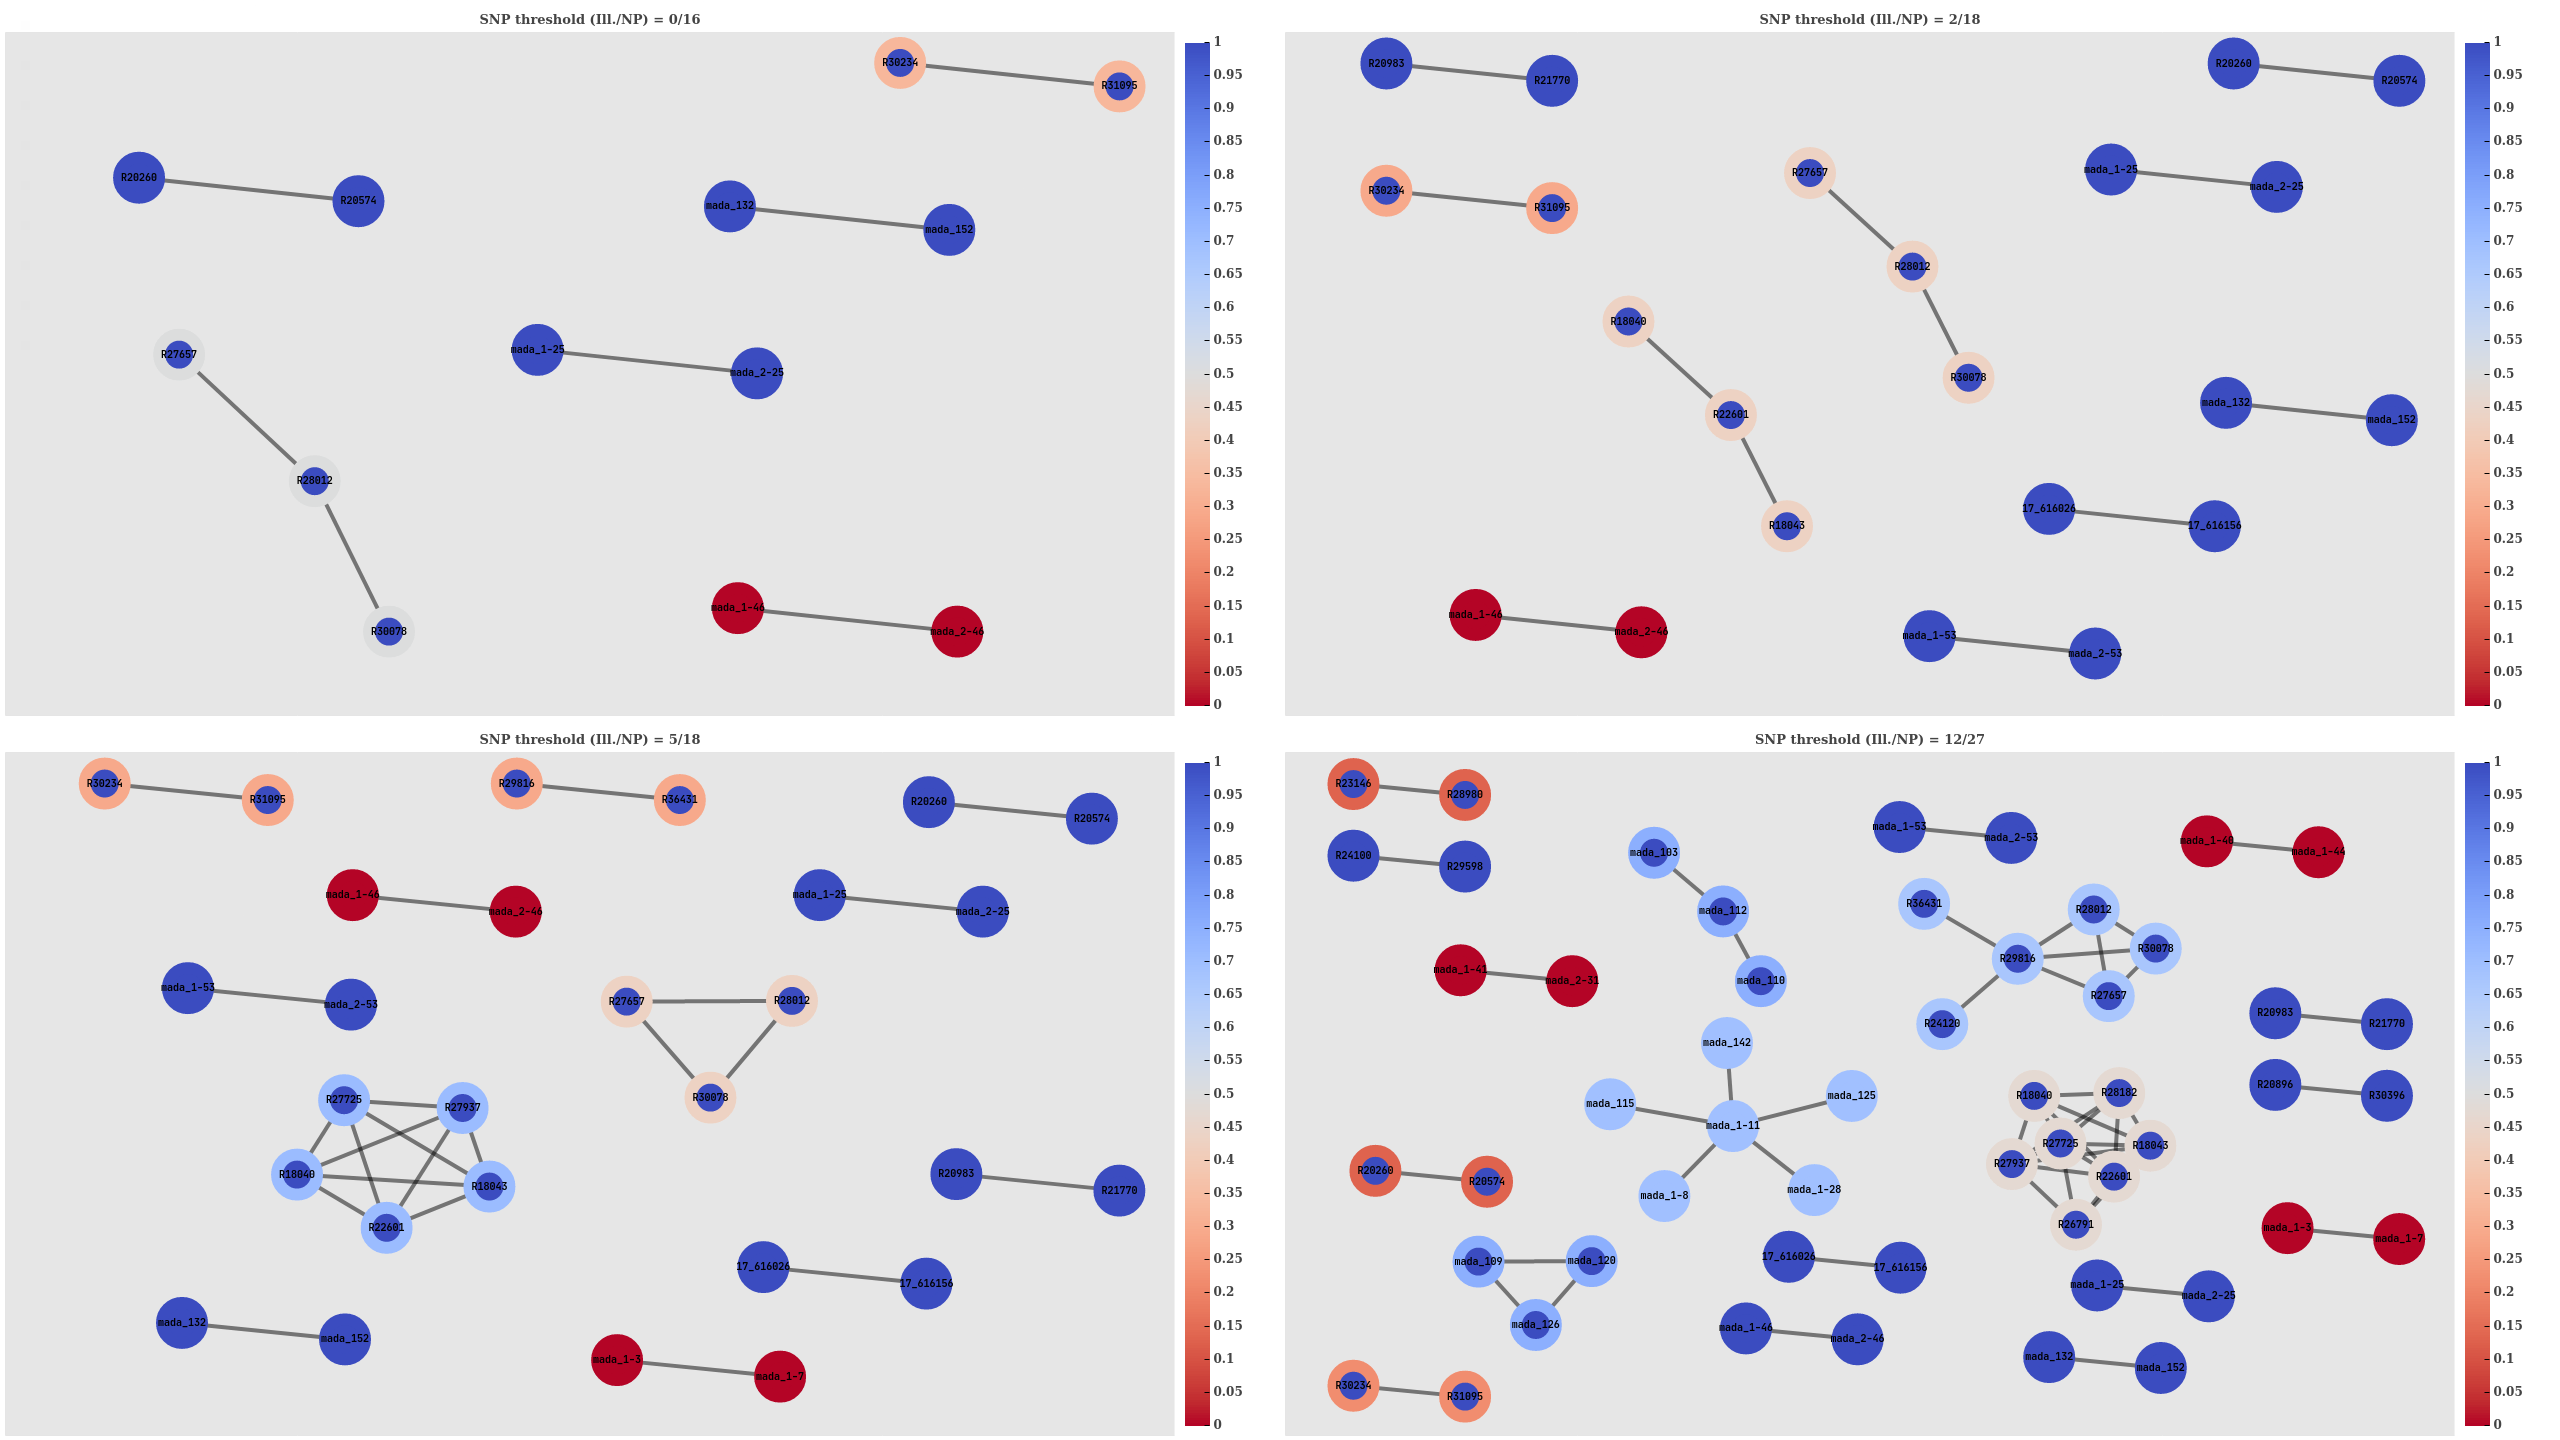
\includegraphics[width=0.90\columnwidth]{Chapter2/Figs/pandora_map_clusters.png}
\caption{{Agreement of Illumina and \pandora{} single-sample (\ont{}) transmission clustering at SNP thresholds 0 (top-left), 2 (top-right), 5 (bottom-left) and 12 (bottom-right). The title of each subplot indicates the Illumina (Ill.) and \ont{} (NP) threshold used when clustering. Samples (nodes) are connected when the SNP distance between them is less than or equal to the relevant threshold. The inner and outer colours for each node indicates the SACR and SACP values, respectively, for its cluster. The Illumina-based clustering is shown.
{\label{fig:map-clusters}}%
}}
\end{center}
\end{figure}

\begin{table}
\centering
\begin{tabularx}{0.95\textwidth}{|Y|Y|Y|Y|} \hline
Threshold & SACR  & SACP  & XCR            \\ \hline
0 (16)    & 0.846 & 0.628 & 0.146 (20/137) \\ \hline
2 (18)    & 0.909 & 0.688 & 0.141 (18/128) \\ \hline
5 (18)    & 0.857 & 0.643 & 0.115 (11/122) \\ \hline
12 (27)   & 0.852 & 0.621 & 0.124 (12/97)  \\ \hline
\end{tabularx}
\caption{Summary of \pandora{} single-sample clustering metrics for four (Illumina) SNP distance thresholds. The threshold(s) in parentheses are the \ont{} equivalent threshold used. The fractions in parentheses for XCR indicate the underlying numbers. SACR=sample-averaged cluster recall; SACP=sample-averaged cluster precision; XCR=excess clustering rate.}
\label{tab:map-cluster-summary}
\end{table}

\subsubsection{Pandora multi-sample}

The SNP thresholds we use for \compare{} clustering are 0, 1, 3, and 7. The results of this clustering are summarised in \autoref{tab:compare-cluster-summary} and visualised in \autoref{fig:compare-clusters}. One important result is that unlike the single-sample approach of \pandora{}, the multi-sample mode leads to perfect SACR across all thresholds. Additionally, clustering at the threshold of 0 perfectly mirrors Illumina. At a threshold of 2, there was one singleton added to an otherwise perfect cluster and two additional clusters of size 2. Thresholds 5 and 12 saw some cluster mergers and singletons forming new clusters or being added to existing ones. The actual clusters produced by \compare{} can be seen in \autoref{fig:compare-original-clusters}.

\begin{figure}
\begin{center}
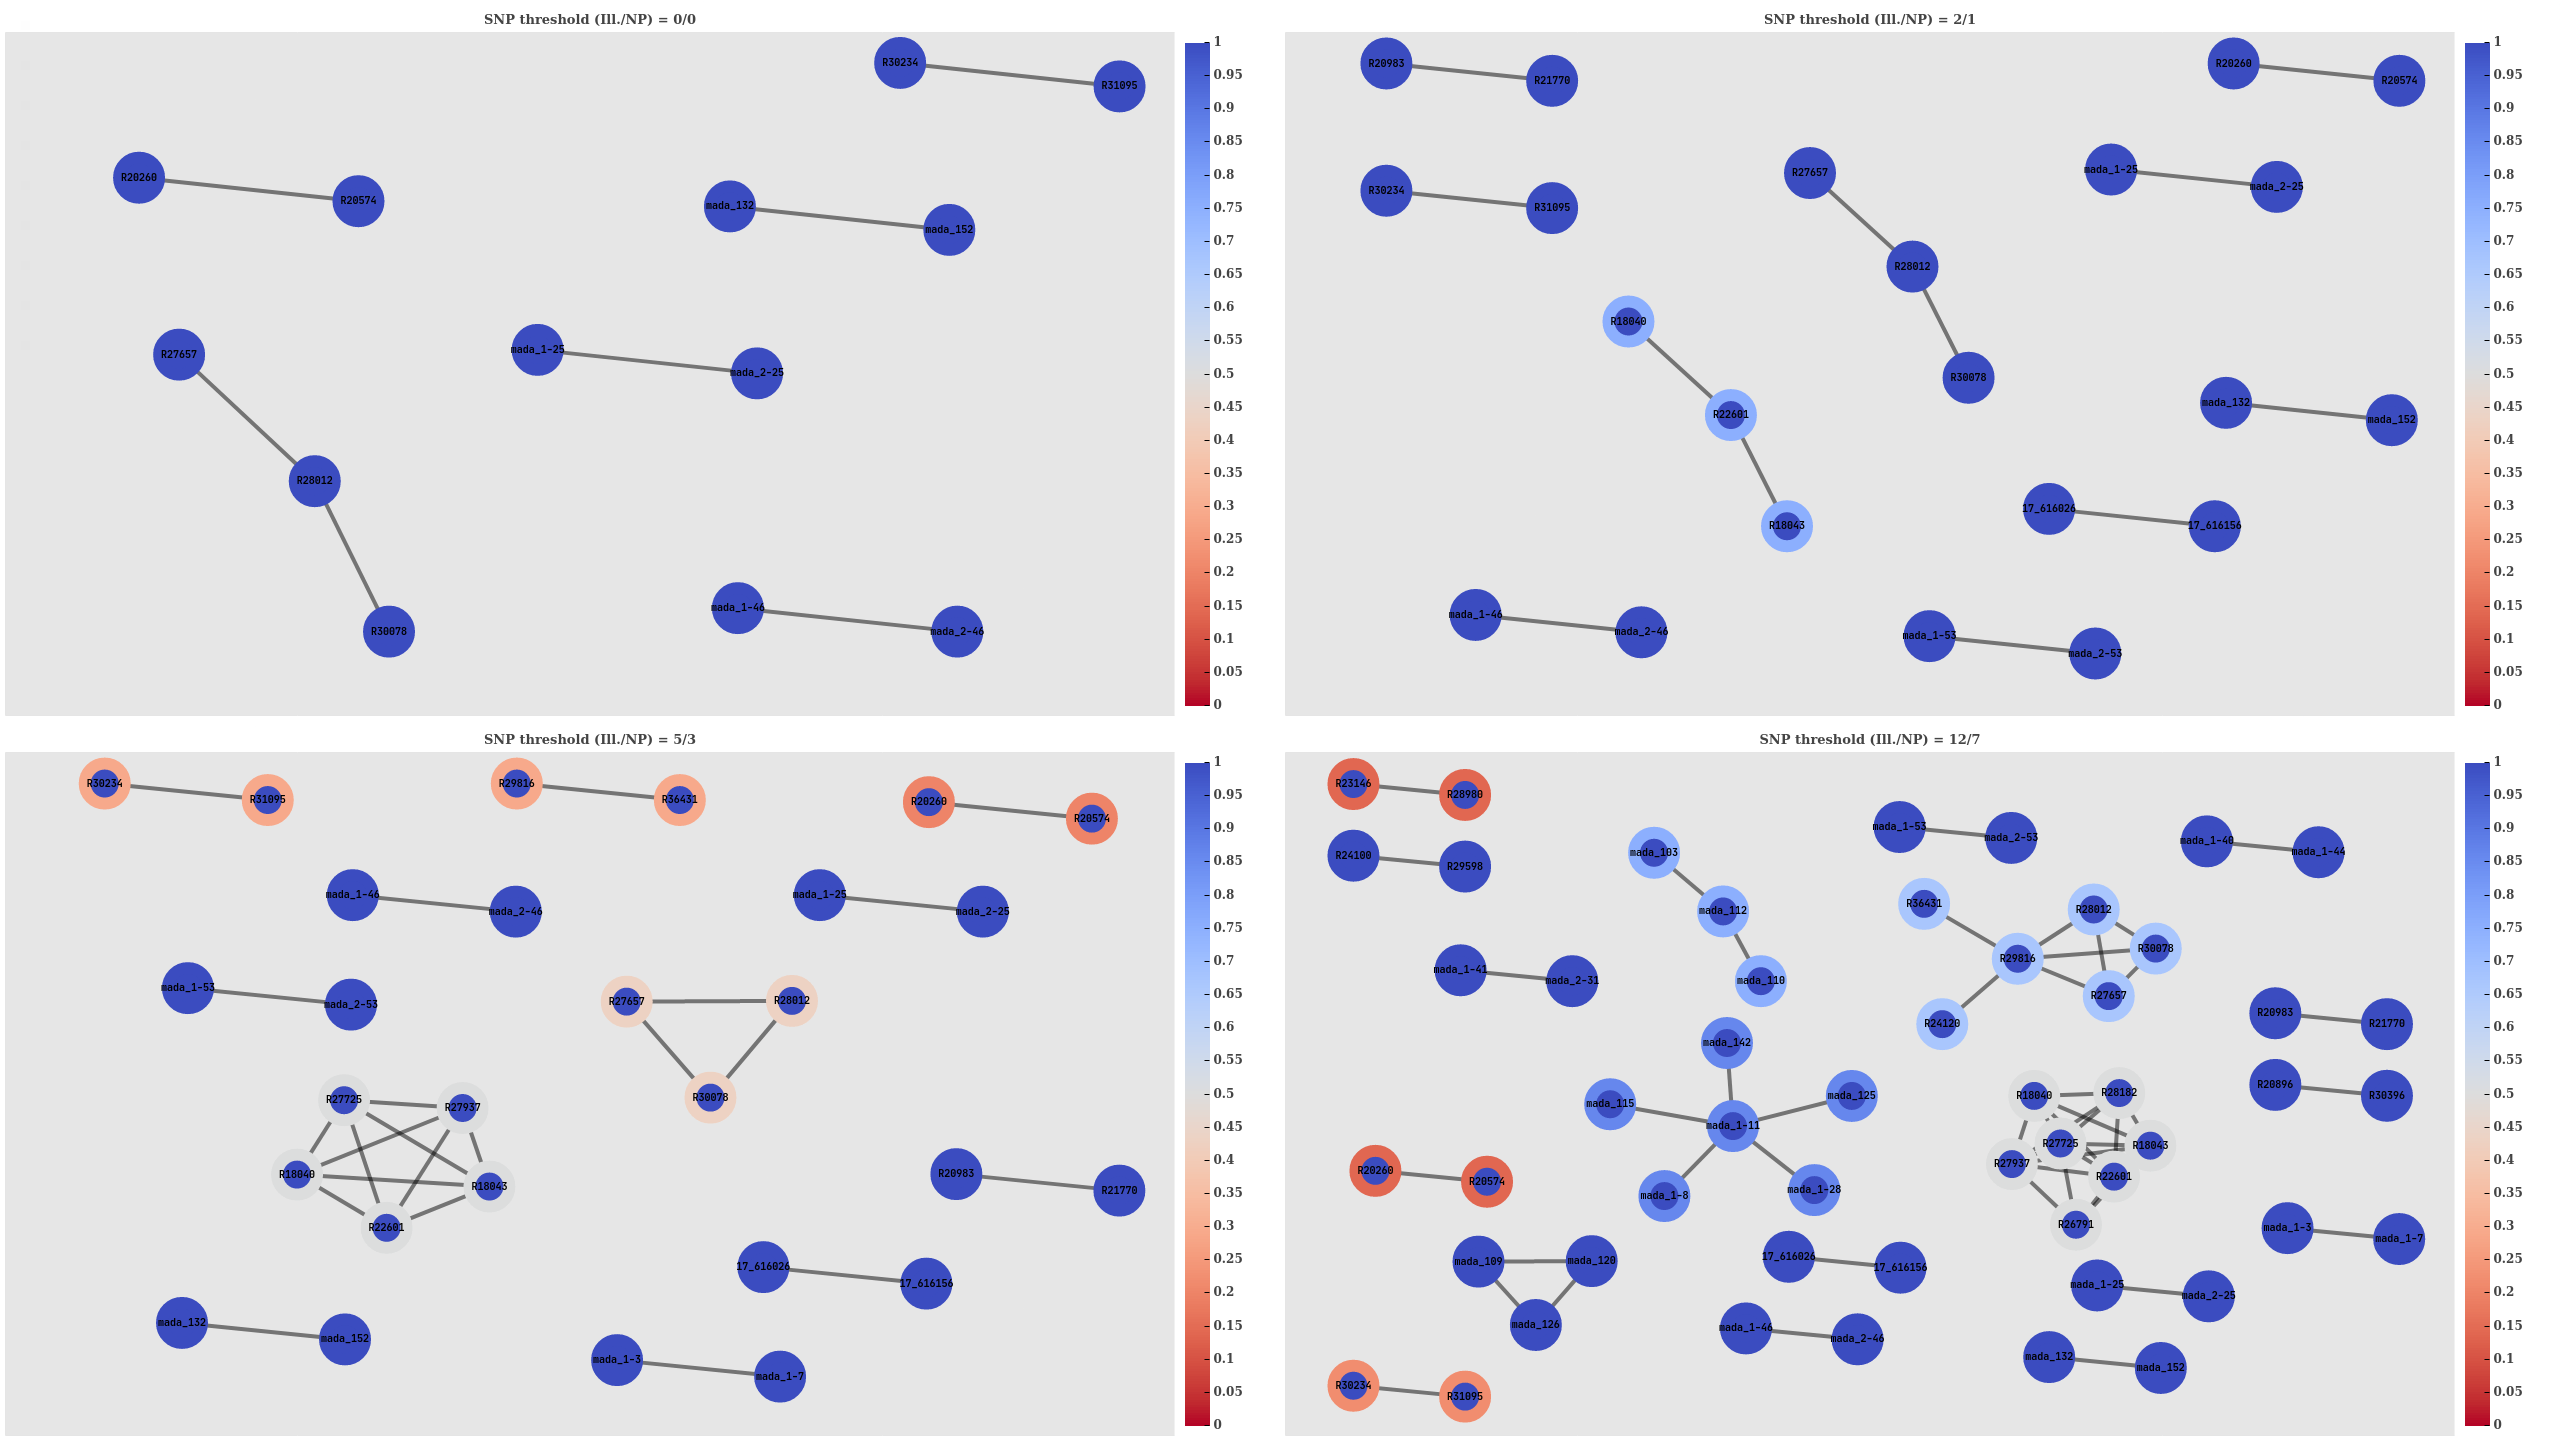
\includegraphics[width=0.90\columnwidth]{Chapter2/Figs/pandora_compare_clusters.png}
\caption{{Agreement of Illumina and \pandora{} multi-sample (\ont{}) transmission clustering at SNP thresholds 0 (top-left), 2 (top-right), 5 (bottom-left) and 12 (bottom-right). The title of each subplot indicates the Illumina (Ill.) and \ont{} (NP) threshold used when clustering. Samples (nodes) are connected when the SNP distance between them is less than or equal to the relevant threshold. The inner and outer colours for each node indicates the SACR and SACP values, respectively, for its cluster. The Illumina-based clustering is shown.
{\label{fig:compare-clusters}}%
}}
\end{center}
\end{figure}

\begin{table}
\centering
\begin{tabularx}{0.95\textwidth}{|Y|Y|Y|Y|} \hline
Threshold & SACR  & SACP  & XCR            \\ \hline
0        & 1.0 & 1.0 & 0.0 (0/137) \\ \hline
2 (1)    & 1.0 & 0.966 & 0.039 (5/128) \\ \hline
5 (3)    & 1.0 & 0.690 & 0.090 (11/122) \\ \hline
12 (7)   & 1.0 & 0.772 & 0.103 (10/97)  \\ \hline
\end{tabularx}
\caption{Summary of \pandora{} multi-sample clustering metrics for four (Illumina) SNP distance thresholds. The threshold(s) in parentheses are the \ont{} equivalent threshold used. The fractions in parentheses for XCR indicate the underlying numbers. SACR=sample-averaged cluster recall; SACP=sample-averaged cluster precision; XCR=excess clustering rate.}
\label{tab:compare-cluster-summary}
\end{table}

\subsection{Summary}
\label{sec:cluster-summary}

The results presented in this section show that when using \bcftools{} for variant-calling, \ont{} is capable of producing transmission clusters with a high degree of similarity to Illumina. Most importantly, no samples deemed part of a cluster by Illumina were missed by \bcftools{}. We have also shown that the Illumina SNP thresholds of 0, 2, and 5 are also valid for \ont{} variant calls from \bcftools{} and the threshold of 12 needs only decrease to 11. 

We also investigated whether the genome graph method of \pandora{} can produce accurate transmission clusters. While the single-sample approach did not yield outstanding results, the multi-sample method shows promise. For all SNP thresholds assessed, \compare{} did not miss any samples from clustering. The SACP values for thresholds 0 and 2 were as good as \bcftools{}, but at thresholds 5 and 12 \compare{} did not perform as well. 

\noindent
In conclusion, we recommend clustering \ont{} data based on \bcftools{} SNP calls for concordant clusters with Illumina.

%=========================================================================

\section{Mixed Illumina and \ont{} transmission clusters}
\label{sec:mixed-clustering}

Having established that \ont{} data can confidently recreate Illumina-defined transmission clusters, we turn to the question of whether this holds when mixing Illumina and \ont{} data. 

Inferring transmission clusters from a mixture of sequencing modalities would allow greater integration across datasets from various sources and prevent laboratories from being locked into one sequencing technology. As the uptake of \ont{} sequencing increases, it seems inevitable that there will be cases where comparisons between these sequencing modalities are necessary. To address this question, we simulate varying degrees of \ont{}/Illumina mixtures and look at how this impacts clustering. To this end, we investigate what the impact (if any) of combining Illumina and \ont{} datasets is on SACR, SACP and XCR (see \autoref{sec:cluster-similarity} for definitions). For the \ont{} data, we use the \bcftools{} distance matrices as they were shown to be the most concordant with Illumina (\autoref{sec:cluster-summary}).

First, we get a sense of how comparable the distances are likely to be by looking at the "self-distance" for each sample - the distance between a sample's Illumina and \ont{} data.  As the sequencing data originate from the same source, we know the self-distance for any sample \emph{should} be 0. However, we also know there are major technical differences between Illumina and \ont{}; therefore, small variability in self-distance is likely. We plot the self-distances in \autoref{fig:self-dist} and see that 64\% (96/150) of the samples have a distance of 0 between their Illumina (COMPASS) and \ont{} (\bcftools{}) data, with 84\% (126/150) less than 2 SNPs apart. All samples have a self-distance of less than 9, except one sample (\vrb{mada\_1-33}), which has a self-distance of 53. We investigated the possibility of a sample mix-up being the cause of this discrepancy but could not find any such convincing evidence. 

\begin{figure}
\begin{center}
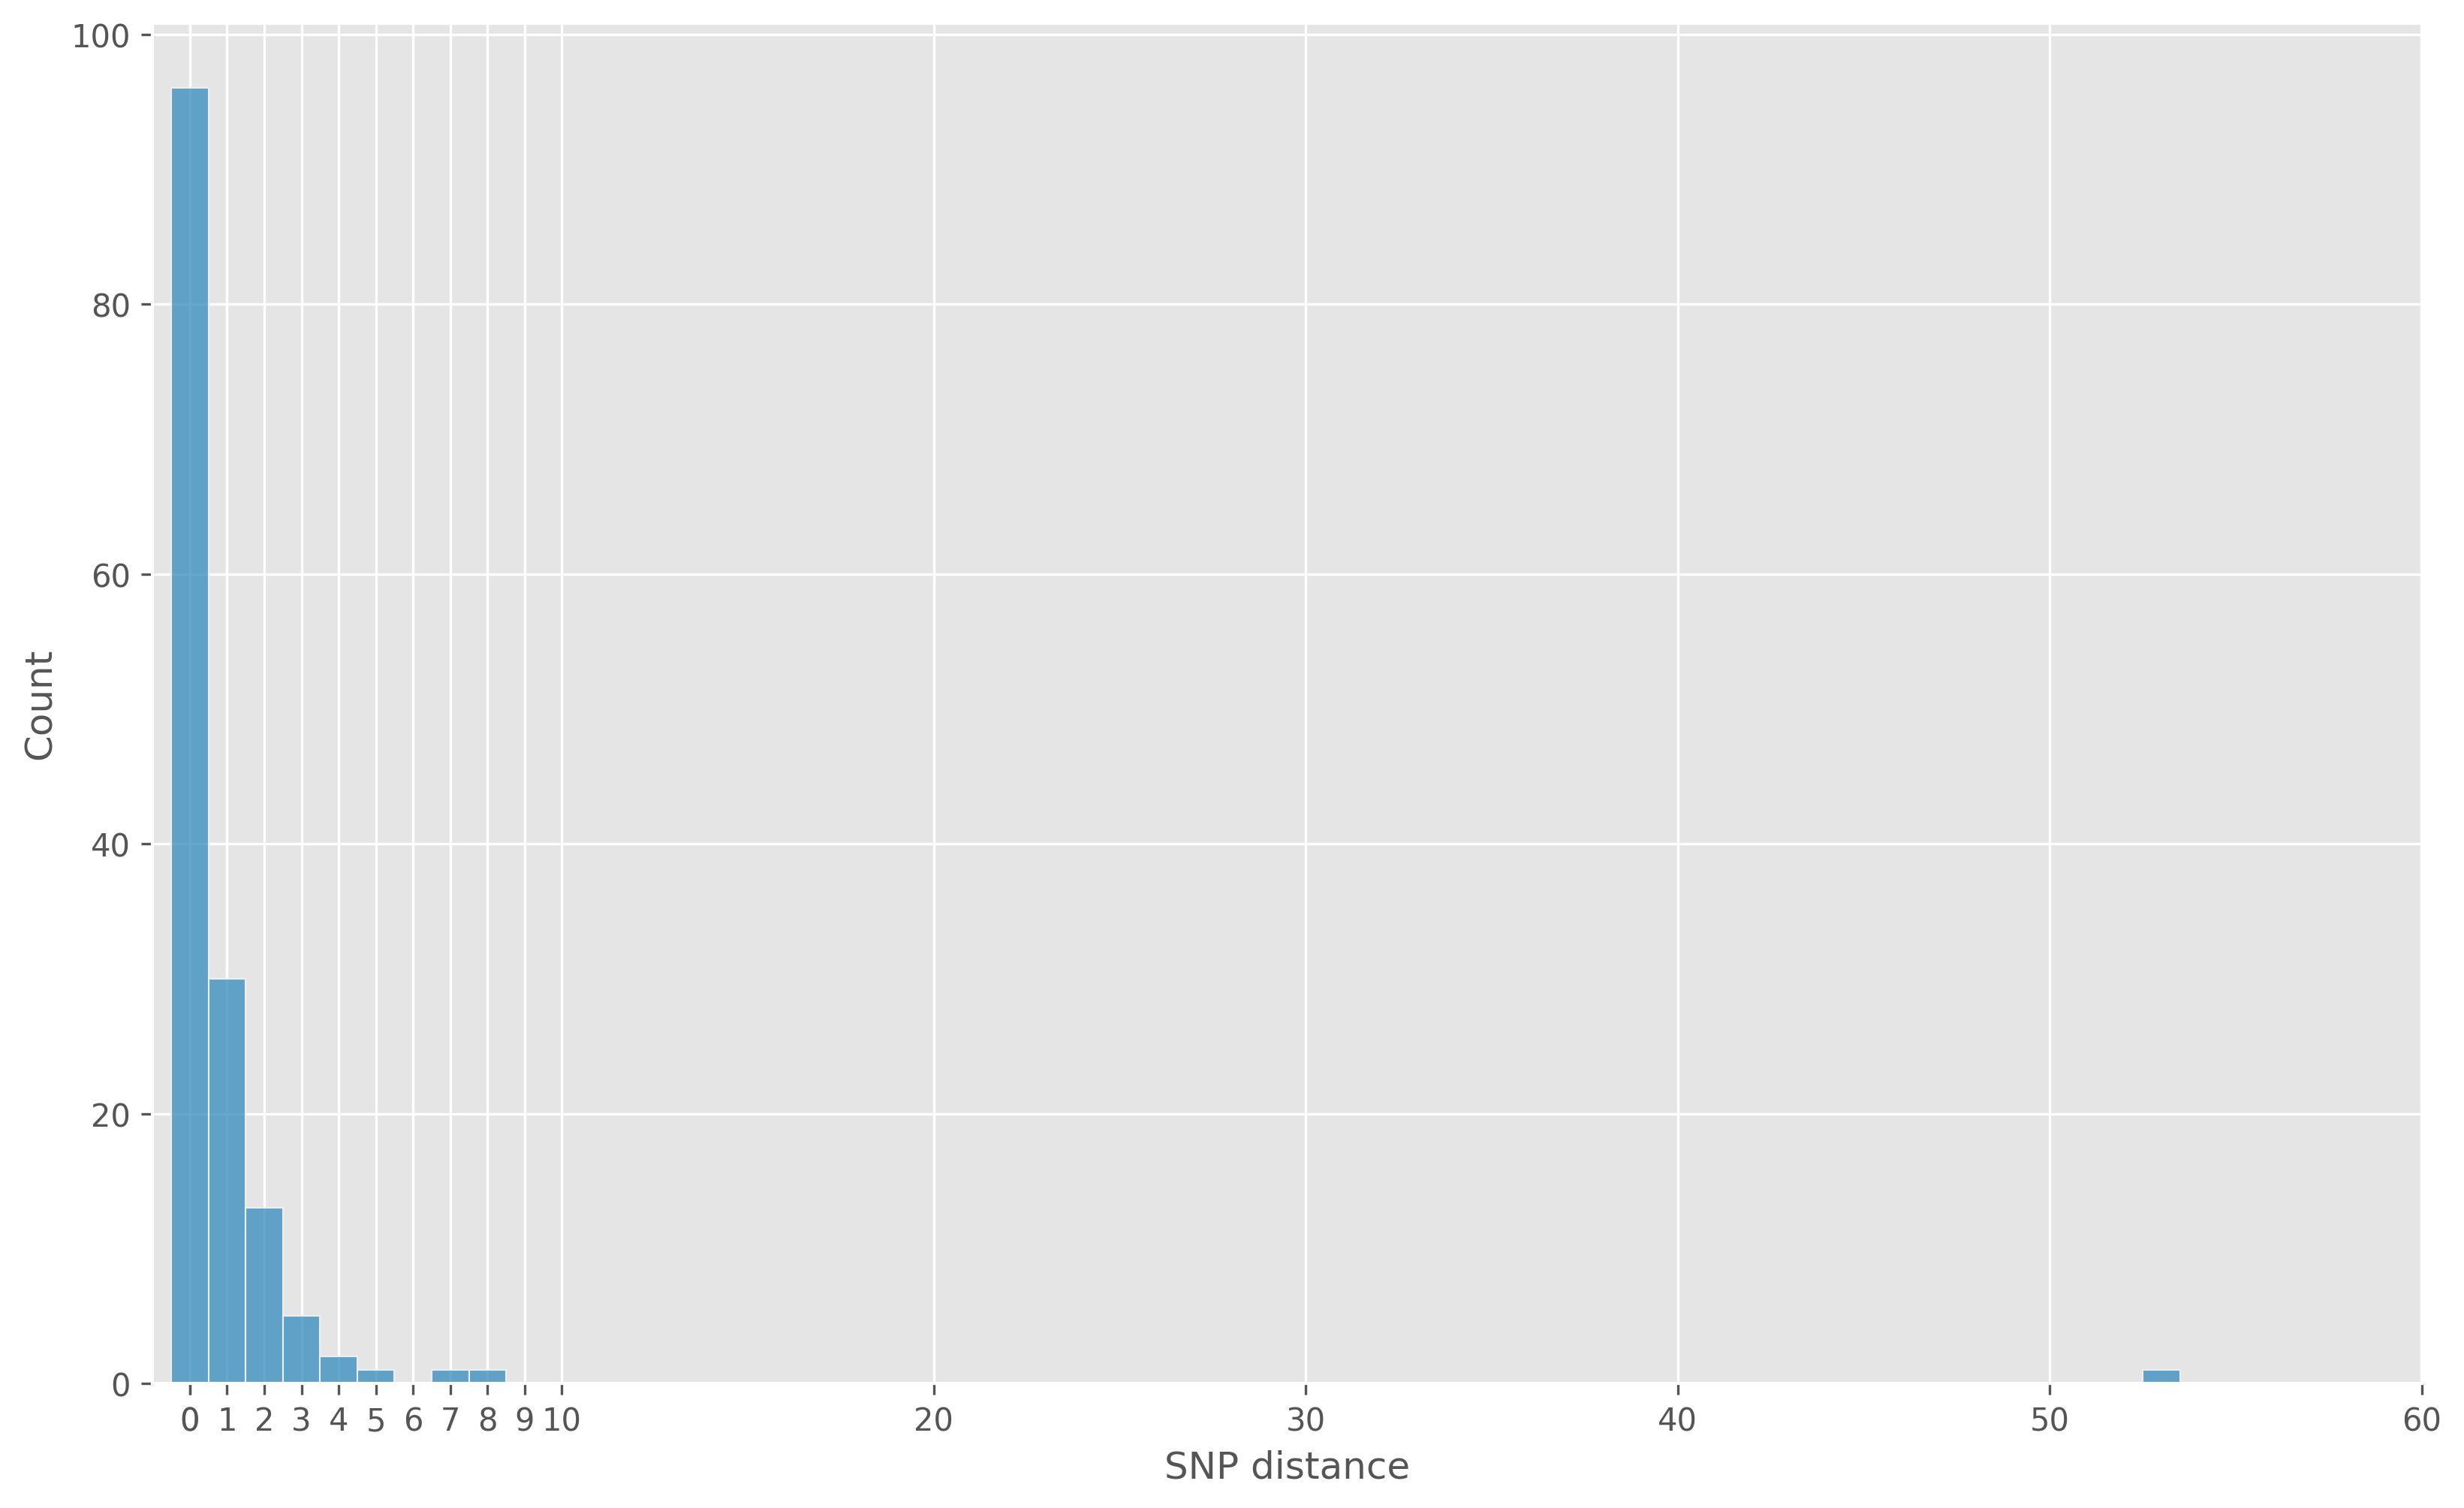
\includegraphics[width=0.90\columnwidth]{Chapter2/Figs/mixed_self_dist.png}
\caption{{Mixed modality "self-distance". This plot shows the SNP distance (x-axis) between each sample's COMPASS (Illumina) and \bcftools{} (\ont{}) VCF calls.
\label{fig:self-dist}
}}
\end{center}
\end{figure}

\noindent
Next, we look at the pairwise SNP distance relationship, akin to that in \autoref{sec:snp-dist}. \autoref{fig:mixed-dotplot} shows the mixed SNP distances have a similar relationship to the single-technology correlation in \autoref{fig:dotplot}. The difference here, however, is that the y-axis represents the distance between one sample's Illumina data and the other's \ont{}. There are twice as many data points in this plot as the distance between two samples is not necessarily reciprocal for mixed modality distances (as we saw with the self-distances). That is, for two samples $a$ and $b$, $distance(a_I,b_N) \neq distance(a_N, b_I)$, where $I$ and $N$ refer to Illumina and \ont{} data respectively. 

In the zoomed inset window of \autoref{fig:mixed-dotplot}, there is a cluster of outlying points with a higher mixed distance than Illumina distance. All of these points relate to combinations of 6 particular samples. We investigated these samples for evidence of a sample swap or low data quality, but nothing was found to support such a claim. In reality, it just seems the \ont{} data for some of the samples are quite different to the Illumina data of the other samples.

\begin{figure}
\begin{center}
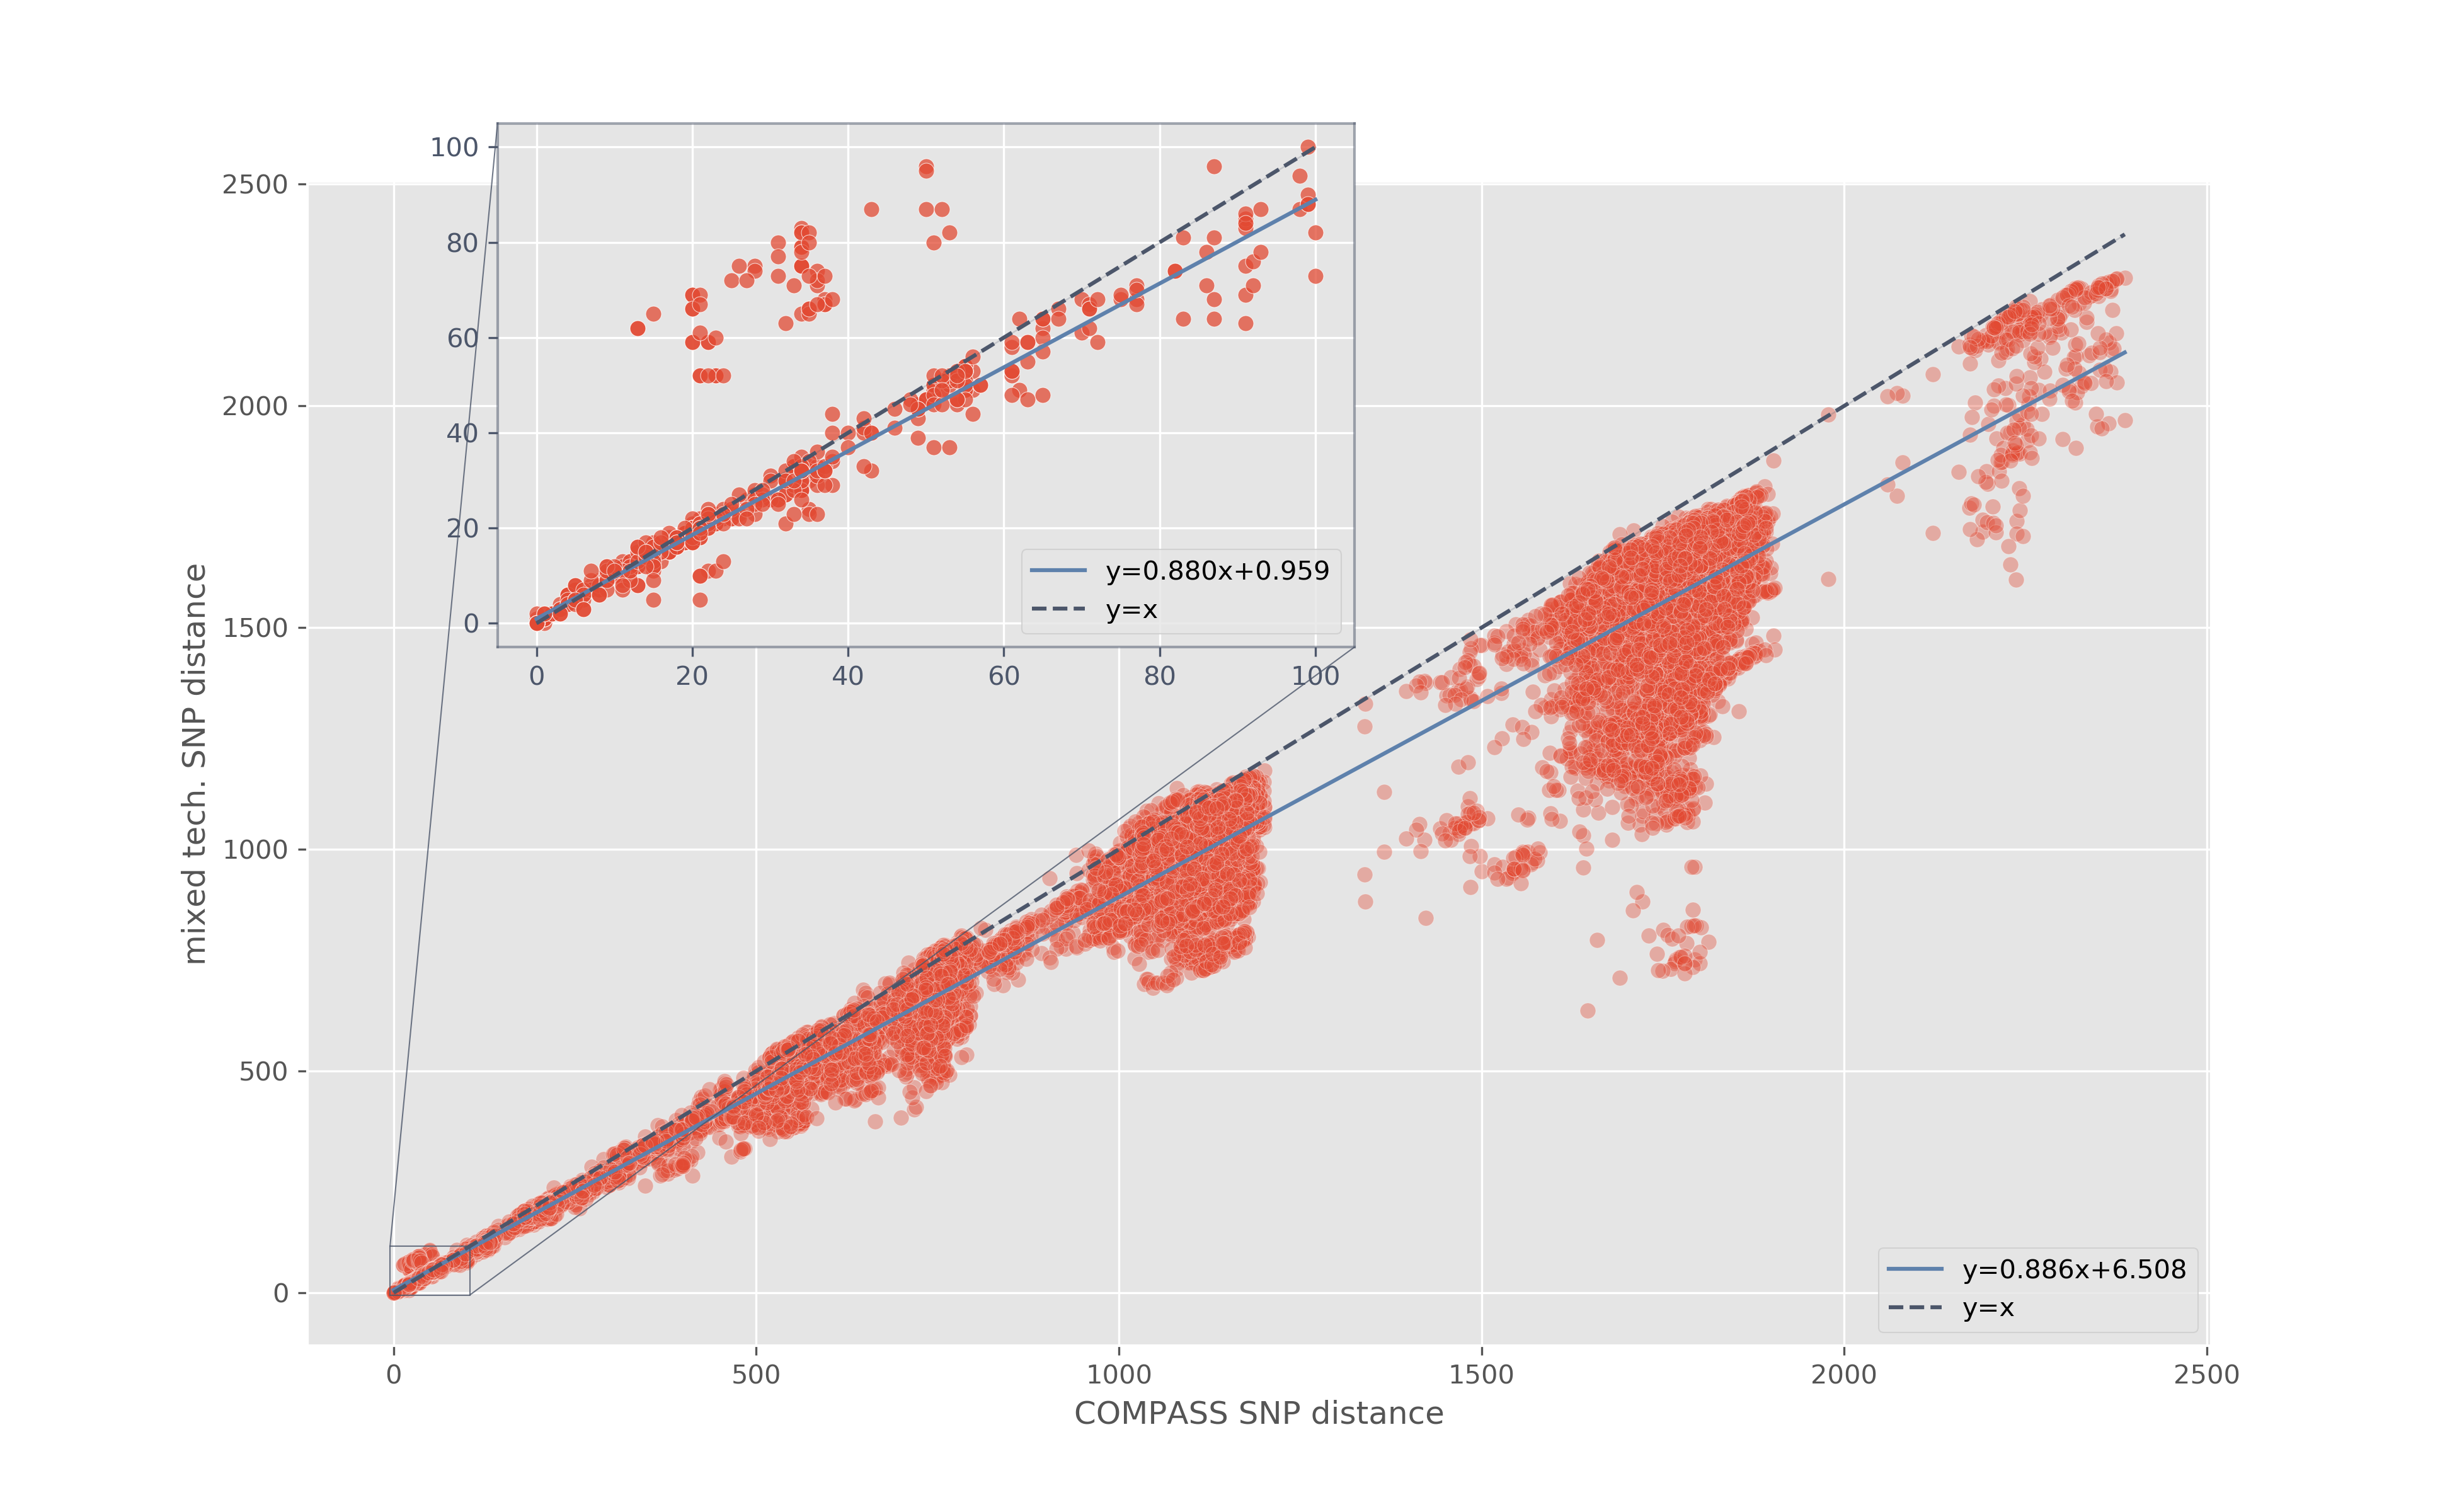
\includegraphics[width=0.90\columnwidth]{Chapter2/Figs/mixed-dotplot.png}
\caption{{The relationship of the distance between all pairs of samples based on Illumina (COMPASS) VCF calls (X-axis) and mixed COMPASS-\bcftools{} calls (Y-axis). The black, dashed line indicates the relationship we would expect if the distance between a pair of samples were the same for both approaches. The blue line indicates the line of best fit based on fitting a robust linear regression model to the data. The inset gives a closer look at the relationship for all sample pairs where the COMPASS distance is less than or equal to 100 SNPs. The legend indicates the linear equations for the lines. Note: to prevent model skew, we do not include self-distance pairs.
{\label{fig:mixed-dotplot}}
}}
\end{center}
\end{figure}

\noindent
We now examine transmission clusters for mixtures of \ont{} and Illumina data using the same SNP thresholds from \autoref{sec:clustering}. The SNP threshold we use when comparing different modalities is the Illumina SNP threshold. The mixture ratios we investigate are 0.01, 0.05, 0.1, 0.25, 0.5, 0.75, and 0.9. That is, for a ratio of 0.25, we \emph{randomly} allocate 25\% of the samples to \ont{} and the remainder to Illumina. For each SNP threshold and ratio, we calculate the XCR, SACR and SACP that the clustering produces. We repeat this process 1000 times for each threshold and ratio to simulate different mixtures of sample/technology pairs. The intention for simulating so many different mixed pairs is to provide insight into how robust clustering is to different ratios of sequencing datasets.  

The results of these simulations are shown in \autoref{fig:mixed-sims} (full summary statistics in \autoref{tab:mixed-sims-full}). We found that for all SNP thresholds and ratios, the median SACR was 1.0. In other words, regardless of the \ont{}/Illumina mixture ratio, for all thresholds we used, no sample is missed from its expected clustering - on average. The SACP values decrease somewhat as the \ont{}ratio increases. However, the lowest median SACP value was 0.845 (threshold 12, ratio 0.9), which is also the SACP value obtained for the \ont{}-only clustering in \autoref{sec:bcftools-clustering} with the same threshold. The XCR values tend to increase slightly with the addition of more \ont{} samples. In the most extreme case, 0.057 was the highest XCR value in any simulation (SNP threshold 5). Incidentally, this is the same as the XCR obtained for the \ont{}-only clustering of the same SNP threshold, which equates to 7 of the 122 non-clustered samples being clustered. However, regardless of the XCR, no samples that should have been clustered were missed (on average).

\begin{figure}
\begin{center}
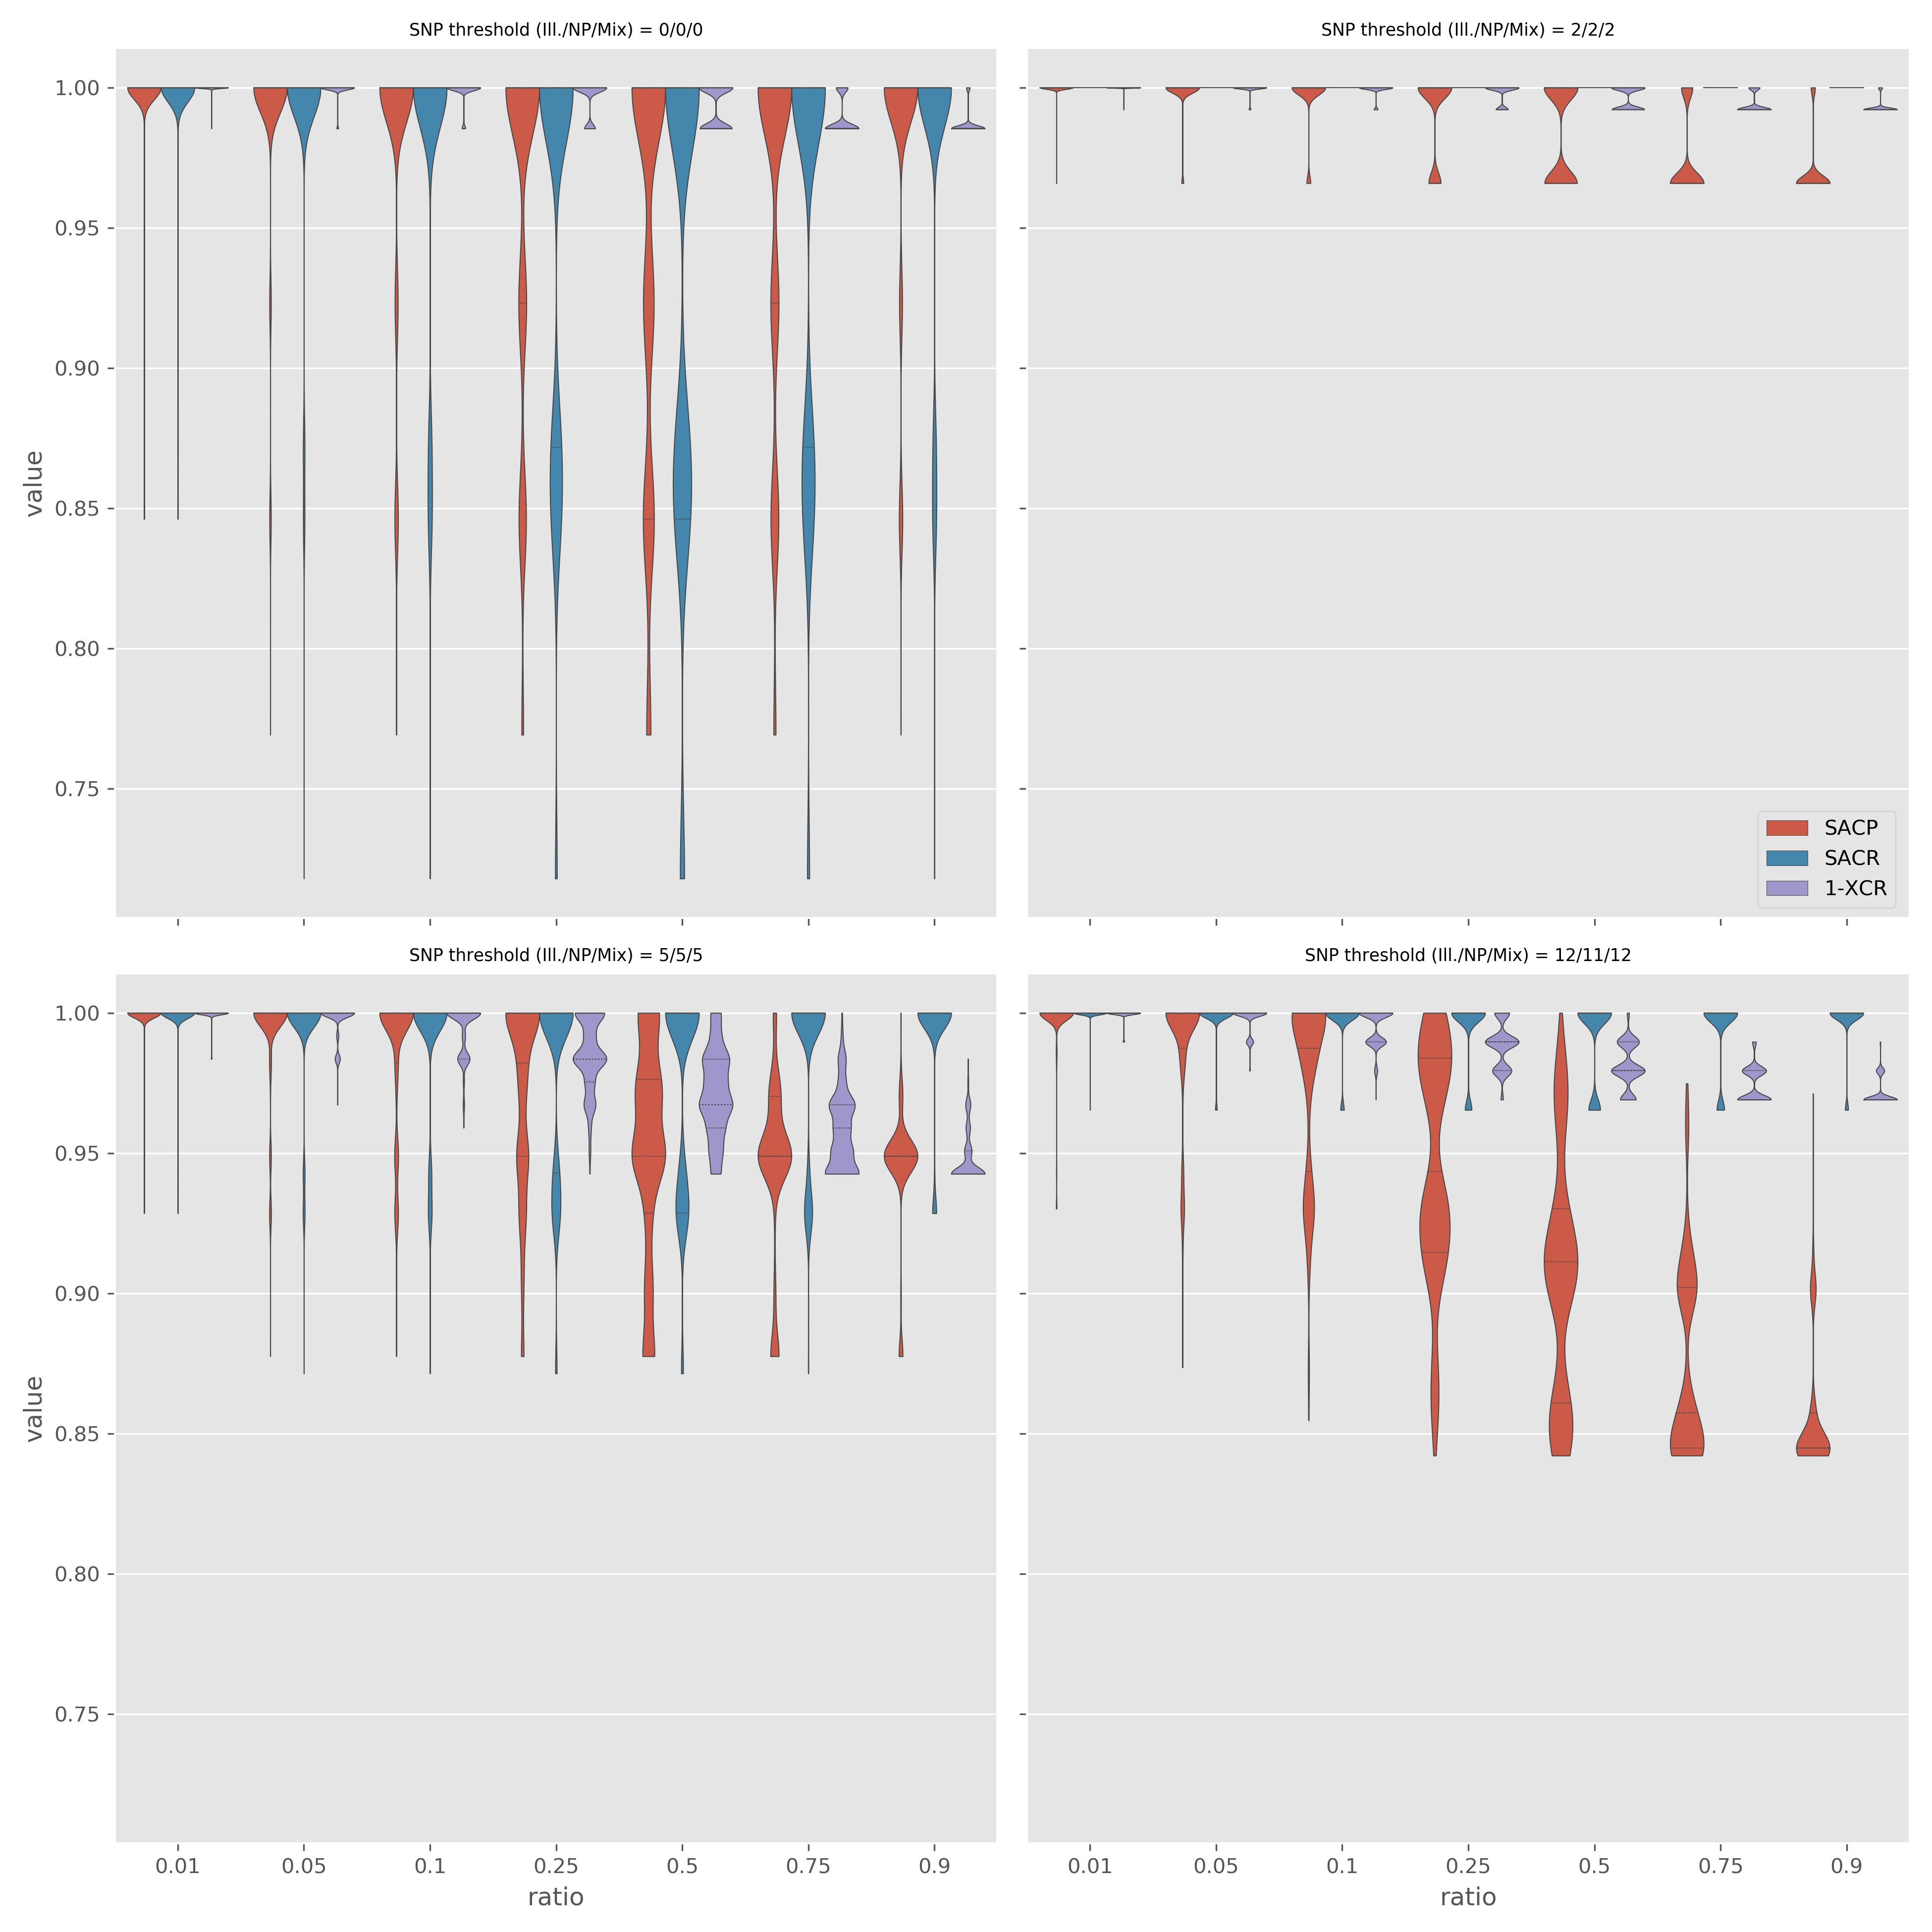
\includegraphics[width=0.90\columnwidth]{Chapter2/Figs/mixed_simulations.png}
\caption{{Simulating various ratios (x-axis) of \ont{}/Illumina sample mixtures. The different thresholds (subplots) indicate the cutoff for defining samples as part of a cluster. The y-axis depicts the Sample-Averaged Cluster Precision and Recall (SACP/SACR) and Excess Clustering Rate (XCR) distributions over all simulation runs (XCR is shown as (1-XCR) for better axis-scaling). For each ratio/threshold combination we run 1000 simulations where the \ont{} and Illumina data is randomly split into the relevant ratio and clusters are defined based on the relevant threshold. The titles for each subplot indicate the SNP threshold used when comparing Illumina (Ill.), \ont{} (NP), or mixed-technology sample pairs.
{\label{fig:mixed-sims}}%
}}
\end{center}
\end{figure}

\subsection{Summary}

In this section, we have shown that putative transmission clusters constructed using mixtures of Illumina and \ont{} data are consistent with those produced by Illumina data alone. As such, datasets from different sequencing technologies can be combined for transmission clustering analysis using the methods in this chapter.

%=========================================================================

\section{Discussion}

Recent work from Smith \etal{} is the first effort to assess \ont{} for the clustering of \mtb{} samples based on genetic distance \cite{smith2020}. While their work had more samples than ours (431), the SNP distance comparison details were very brief and only presented for a subset of 14 samples. They present the results as a distance matrix and leave it as an exercise for the reader to compare the Illumina and \ont{} matrices. There is no quantification of the clustering similarities or investigation into whether Illumina and \ont{} data can be mixed for this application. In contrast, the work presented in this chapter provides a detailed analysis of all of these topics - and more.

In addition to the conventional single-reference variant-calling approach, we also assessed the performance of the genome graph method presented in \autoref{chap:denovo}, for \mtb{}. We built two \mtb{} population reference graphs with different variant densities. Intuition would say that the more variants in the \prg{}, the better the ability to find and call variants. However, we found the opposite. The sparse \prg{} produced marginally higher precision and recall, on average, compared to its dense counterpart. As the computational resources required to construct and operate the sparse \prg{} are a lot less than the dense, we chose to use it for the subsequent analysis. The lack of improvement by adding more variants is consistent with previous work from Pritt \etal{}, who found a ceiling in gains by adding more variants \cite{pritt2018}. They note that eventually, the extra variants cause complexity "blow-ups" that manifest as increased computational resource requirements and reference ambiguity, all of which lead to a decay in overall performance. This reduction in performance is the same thing we see. Many of the errors made by the dense \prg{} relate to shared \kmer{}s between alternate paths through sites in the graph. These shared \kmer{}s, in turn, confuse the genotyping by adding coverage to multiple alleles. We discuss this further in \autoref{sec:improve-prg} and investigate this complexity problem further in \autoref{chap:dst}.

The initial step in this chapter was the first investigation of the precision and recall of \ont{} variant calls for \mtb{}. Previous work from Bainomugisa \etal{} has only looked at one sample and assessed variants in the \ppe{} genes \cite{bainomugisa2018}. While there are several \ont{} variant callers recently published, we chose to use \bcftools{} due to its similarity to the Illumina strategy we are comparing to and for its ease of use. Many of the \ont{} variant callers are neural network-based and require considerable bioinformatics knowledge to operate and, in some cases, require training of variant models. As our goal in this chapter is to investigate the use of \ont{} by public health laboratories (and for clinical purposes), we try to use methods that can be easily duplicated by others who may not have extensive bioinformatics training. It is difficult to directly compare our precision and recall values to other \ont{} variant-calling studies as we value precision higher than recall for the work in this chapter. Much of the \ont{} variant-calling benchmarks focus on balancing precision and recall. The precision from both \ont{} variant-calling strategies we analysed were consistent with Illumina and much higher than previous \ont{} benchmarks \cite{clair2020,clairvoyant2019}. However, we acknowledge the unfair comparison to other works given the different focus. Recall for both \bcftools{} and \pandora{} were lower than Illumina - by quite a lot for \pandora{}. Compared to other \ont{} variant-calling work, the recall values we can obtain are a few percentage points below the best \cite{sanderson2020,clair2020}. Given that we also report results for various variant filtering levels, we hope these can be used by others who may place a higher value on recall.

One unfortunate limitation of the variant-calling validation was the number of PacBio assemblies we could use. We sent 35 samples for PacBio sequencing, but we only received sufficient data for the assembly of 9 samples - and two of those failed QC due to technical difficulties in the sequencing lab. These results would have been even more robust with 35 validation samples; however, seven is comparable with the numbers used in other \ont{} variant calling evaluation work \cite{sanderson2020,clair2020,clairvoyant2019}.

We have outlined three new metrics for comparing the similarity of two transmission clustering approaches, the sample-averaged cluster recall (SACR) and precision (SACP), and the excess clustering rate (XCR). SACR and SACP are derived from the set-similarity measure, the Tversky Index \cite{tversky1977}. XCR has not been described elsewhere to the best of our knowledge. Cluster similarity is a rich field of research, yet, there are not many examples of this quantitative approach to comparing transmission cluster methods. Of the studies that \emph{do} compare clusters between methods, none provide the level of information provided by SACR, SACP, and XCR collectively. Meehan \etal{} use a clustering rate metric, which is the number of samples clustered, minus the number of clusters and then divided by the number of samples \cite{meehan2018}. Roetzer \etal{} focused on manually comparing a single large cluster but did not compare all clusters \cite{roetzer2013}. Perhaps the closest to our approach is that by Stimson \etal{} \cite{stimson2019}, who use an information theory metric called variation of information (VI) \cite{meila2007}. VI works well and is not too dissimilar to our approach. It measures how much information is lost and gained in between two clustering approaches.

Our main reason to forego these previous methods in favour of our three has to do with the granularity of information. The studies mentioned all use a single metric to classify the performance of the clustering. However, using SACR, SACP and XCR, we see how changes in the methods for producing clusters impact whether samples are missed from clusters (SACR), wrongfully added to existing clusters (SACP), or if previously unclustered samples form new clusters (XCR). Such granularity allows users to tweak their clustering approach to meet their situation. For example, while we place a higher value on SACR, others may find the reduction of cluster merging is of more importance and can focus on improving SACP instead. A single metric does not allow for this kind of targeted evaluation.

The first important finding of this chapter is that \ont{} data can produce transmission clusters comparable to Illumina. Indeed, \bcftools{} and \compare{} do not miss any samples from clusters - the most important consideration for transmission chain investigation \cite{walker2013}. This result agrees with the only other \mtb{} study of this kind \cite{smith2020}. Additionally, \ont{}'s suitability for transmission investigation has been confirmed for other pathogens such as Human metapneumovirus \cite{xu2020}, Shiga toxin-producing \ecoli{} (STEC) \cite{greig2021}, and \textit{Neisseria gonorrhoeae} \cite{sanderson2020}.

It is essential to highlight that the focus of this work is not as a variant-calling benchmark for WGS technologies. We acknowledge that COMPASS may not be the best Illumina-based variant calling strategy. Indeed, there are many bioinformatic pipelines available for the analysis of \mtb{} Illumina data, all with different results from one another \cite{walter2020}. Instead, we take an approach used by PHE and ask whether \ont{} can provide information of the same quality. For the application of clustering \mtb{} genomes based on genetic distance, we find \ont{} does provide comparable information when using \bcftools{} to call variants. In addition, we found that using the multi-sample comparison mode of \pandora{} we also succeed in clustering all samples that should be clustered, albeit at the cost of adding more false-positive connections. 

While the precision of variant calls for \pandora{} was as high as Illumina, the clustering produced by the single-sample mode (\vrb{map}) was much worse than the other approaches. In general, the distances between samples based on \pandora{} \vrb{map} variant calls were much higher than the Illumina data implied they should be. One point that contributes to this difference is the subtle difference in how we generate the \pandora{} \vrb{map} consensus sequences. The main difference compared to \bcftools{} and Illumina is that when a position in the H37Rv reference genome is missing from the \pandora{} \vrb{map} VCF, we assume it is the reference position, rather than nullifying it as we do with COMPASS and \bcftools{}. We initially took the nullify approach for missing positions but found this lead to a substantial under-calling of the distances. The bulk of the extra pairwise differences (false positives) called by \pandora{} \vrb{map} were positions missing from one of the samples and present in the other. 96\% of those false-positives positions were filtered out in the COMPASS and \bcftools{} VCFs due to evidence of heterozygosity. Ultimately, this issue stems from the fact that COMPASS and \bcftools{} make calls at all positions of the genome (with read depth), while \pandora{} only makes calls at sites with alternate alleles. A new approach for calculating the distance between \pandora{} single-sample VCFs certainly warrants further investigation.

The difference in clustering obtained by the two \pandora{} approaches highlights their intended use cases. The multi-sample approach, \compare{}, was designed for allowing the comparison of collections of samples. It integrates information from \emph{all} samples by selecting a consensus sequence that best approximates them and then calls variation against that consensus. This approach allows for easily identifying differences between samples as the VCF produced by \compare{} has genotype information for all samples at all sites. While \compare{} did not miss any samples from their correct clusters, it did incorrectly join some clusters and create new clusters from samples Illumina deemed singletons. This incorrect joining of samples and clusters is not entirely unexpected. Incorrectly joining samples indicates that the distances between samples are lower than expected for \compare{} (this is supported by \autoref{fig:dotplot}). Given the \pandora{} variant calls showed significantly lower recall than COMPASS and \bcftools{} (see \autoref{fig:prec-recall-filters}), a smaller distance between samples is expected. One obvious way of trying to improve recall is by masking less of the genome (see \autoref{app:mask}). 

In addition to acknowledging that this variant-calling approach may not be the absolute best approach, we also acknowledge that SNP distance clustering has shortcomings. Again, our intention is not to claim to be the best clustering method but to mimic the process currently used by PHE - which is the SNP threshold approach used here. Stimson \etal{} recently published a notable study showing that combining a SNP threshold approach with epidemiological data can lead to superior transmission chain reconstruction compared to SNP threshold alone \cite{stimson2019}. With the establishment of \ont{}'s ability to provide accurate SNP threshold-based clusters, it seems certain that the inclusion of epidemiological data using the same approach as Stimson \etal{} can only improve inference for this application.

With the knowledge that \ont{} can infer likely chains of transmission for \mtb{} we ask a logical next question: can transmission clusters be accurately constructed from a mixture of \ont{} and Illumina data? As \ont{} sequencing increasingly pervasive, it seems inevitable that groups using different sequencing modalities will want to compare data. We find that they can be mixed and produce clusters consistent with Illumina-only data. 

This analysis is the first known case (to the author's knowledge) of testing this mixing of data for \mtb{}. The mixture of \ont{} and Illumina consensus sequences have been investigated for hepatitis C \cite{riaz2021}, and STEC \cite{greig2021}, with the authors also finding the modalities can be mixed without degradation of results. Others have also compared phylogenetic trees constructed from a combination of the two modalities \cite{lijun2020,McNaughton2019,greig2021} with similar findings. Perhaps the unique insight from our work is that we assess the effect of different mixture ratios on clustering. 

Another interesting insight from this study of technology mixtures is self-distance (\autoref{fig:self-dist}). In their work on \textit{N. gonorrhoeae}, Sanderson \etal{} found a median self-distance of 5, with a range of 1-10 and interquartile range (IQR) of 3-6 ($n=8$) \cite{sanderson2020}. While Greig \etal{} saw self-distances of 5 and 6 ($n=4$) in STEC \cite{greig2021}. In contrast, we found a (\bcftools{}) median self-distance of 0 with an IQR of 0-1 ($n=150$). Our range was 0-53, and with the outlier of 53 removed, the range becomes 0-8. Both of these studies used similar variant filtering strategies to ours, except with different variant callers - highlighting the need for continued standardisation of \ont{} variant calling, or even recommendations for specific species.

%=========================================================================

\section{Conclusion}

In conclusion, the work in this chapter has shown that \ont{} data can produce transmission clusters consistent with those from Illumina. Additionally, it is also possible to mix data of the two modalities and produce concordant clusters. Finally, we provide the first evaluation of \ont{} variant-calling for \mtb{}, and three new metrics for assessing transmission cluster similarity.

These results are consistent with another \mtb{} \ont{}-based transmission cluster study and similar work on other bacterial and viral pathogens. As a result, we believe \ont{} sequencing has reached sufficient quality to be considered for public health investigation of transmission clusters.

%=========================================================================

\section{Future work}

\subsection{Dataset with known epidemiological information}
Perhaps the most important follow up of the work in this chapter is to gather a dataset with epidemiologically linked cases and known transmission clusters. While these datasets do exist for Illumina data, there are none yet with matched Illumina and \ont{} sequencing. Matched sequencing data is necessary to know that differences in DNA are solely driven by sequencing technology. A dataset with solid evidence for transmission clusters would remove the main limitation to this chapter and be an even stronger statement for the use of \ont{} sequencing in public health laboratories.

\subsection{Computational performance of variant calling}
\label{sec:fw-comp-perf}
% bcftools baq work https://github.com/mbhall88/head_to_head_pipeline/issues/38#issuecomment-661680608
In \autoref{sec:var-call-comp-perf} we assessed the time and memory usage for variant calling with \bcftools{} and \pandora{}. \bcftools{} in particular had, in the worst case, the highest memory and CPU of the callers. Nearly all of this time and memory is spent realigning reads in the pileup in order to calculate the base alignment quality (BAQ) score \cite{li2011}. When we disabled this BAQ setting for one sample, the CPU time dropped from 3 hours to 30 minutes (6-fold decrease) and peak memory reduced from 58GB to 70MB (829-fold decrease). However, this did come at the cost of a slight reduction in precision and recall. As we write this chapter, the newest release of BCFtools (version 1.13) has addressed this problem by only doing the BAQ realignment in areas overlapping problematic indel sites. Their testing shows this drastically reduces the peak memory and overall runtime and \emph{increased} recall (the realignment can sometimes be detrimental). As such, an obvious task for future development would be to rerun this analysis with the latest \bcftools{} version and assess the expected changes in computational resource usage and recall.

Much of the memory and CPU time in the \pandora{} pipelines lies in updating the multiple sequence alignments used to build the \prg{} after novel variants have been added. Recent work by Leandro Ishi in our research group has produced a prototype of the \makeprg{} program that significantly reduces the time and memory required to update the \prg{} (as discussed in \autoref{sec:denovo-fw}). It remains to be seen whether these updates will also improve \pandora{}'s precision and recall, but it will undoubtedly improve the computational requirements. 

\subsection{Improving \prg{} construction}
\label{sec:improve-prg}
The current process for building the \mtb{} \prg{} is, for each locus, to apply a single VCF alternate allele to the reference sequence for that locus and collect all of these mutated sequences into a multi-sequence FASTA file. One limitation of this approach is that variants do not always occur in isolation like this. Where this becomes important is when turning an MSA into a \prg{} with \makeprg{}. An important parameter in this process is the minimum match length, $m$. When two variants are within $m$ positions of each other, creating two separate sequences for them (as we do) creates alternate paths in the \prg{}, with neither path containing the correct allele combination. This situation is best understood with an example. We set $m$ to 3 and have two variants at positions 2 and 4 - in a hypothetical genome sequence \vrb{AAAC}. The first variant is a SNP changing an \vrb{A} to a \vrb{T} and the second a \vrb{C} to a \vrb{G}. The two mutated sequences we produce for these two variants are \vrb{ATAC} and \vrb{AAAG}. Because these two sequences do not have a minimum match length of 3 or more, they become two alternate paths in the \prg{}. However, these two variants come from the same sample, so in reality, the true sequence is \vrb{ATAG}. When using the \prg{} containing the two alternate alleles, if we have a sample that contains both of the variants (i.e., \vrb{ATAG}), it does not match either of the two alleles in our \prg{}, even though they come from a sample with \vrb{ATAG} at this site. Ultimately, we rely on the \denovo{} variant discovery from \autoref{chap:denovo} to fix this. Unfortunately, this does not always work and, as we will see in \autoref{chap:dst}, even if \denovo{} discovery adds the correct allele combination, \vrb{ATAG}, we now have three alleles that could share minimizing \kmer{}s. Having shared minimizers over multiple alleles at the same position can lead to read coverage across all of those alleles - ultimately skewing genotyping. 

One way to minimise these excess alleles would be to construct the \prg{} by producing a single sequence at each locus from \emph{all} variants for a sample - rather than a sequence for each variant. The reason we did not construct the \prg{} in this fashion in \autoref{sec:tbprg} was that for each locus, we would have had to perform an MSA on $n$ sequences - where $n$ is the number of samples. Instead, we chose to apply single variants as the number of variants in a locus was, in most cases, \emph{much} smaller than $n$ and thus, the MSA ran quicker and used much less memory.

In addition to improvements in variant inclusion, some changes can be made in the masking of loci. Our current method of removing loci from the \prg{} when they have 30\% or more overlap with a genome mask (\autoref{app:mask}) leads to approximately 6\% of loci being removed - 10\% of the genome. As the genome mask used covers 7.4\% of the genome, we remove more than is necessary, which impacts our recall. A recent study by Marin \etal{} has shown this genome mask to be excessive, and they present a new mask that covers only 4\% of the H37Rv reference genome \cite{marin2021}. So a first step for improving the recall of \pandora{} would be to rebuild the \prg{} using this new mask.

%=========================================================================

\section{Availability of data and materials}

The pipelines and scripts used in this chapter are available at \url{https://github.com/mbhall88/head_to_head_pipeline}. A special mention must go to the workflow management program \vrb{snakemake} \cite{snakemake2021}, which was used to coordinate all analyses. All figures were generated using the Python libraries \vrb{matplotlib} \cite{matplotlib}, \vrb{seaborn} \cite{seaborn}, and \vrb{bokeh} \cite{bokeh}.

\towrite[inline]{availability of the data if it has been deposited prior to submission}